%!TEX root = main.tex

\section{Application Fields and Examples}

\begin{frame}{Application Fields and Examples}{Bechmarking the Index Reduction Algorithm}
  \hic{The benchmark problems \dots}
  \begin{columns}
    \hspace{0.035\textwidth}
    \begin{column}[t]{0.575\textwidth}
      \textbf{Multi-body dynamics}
      \begin{enumerate}\small
        \item Car-axis (index-3)
        \item Flexible slider-crank (index-3)
        \item Double-wishbone suspension (index-3)
      \end{enumerate}
      \textbf{Trajectory prescribed path control problems}
      \begin{enumerate}\setcounter{enumi}{3}\small
        \item Space shuttle initial stage reentry (index-3)
        \item Space shuttle final stage reentry (index-2)
        \item Robotic arm control  (index-5)
      \end{enumerate}
    \end{column}
    \hspace{-0.055\textwidth}
    \begin{column}[t]{0.55\textwidth}
      \textbf{Electric circuits}
      \begin{enumerate}\setcounter{enumi}{6}\small
        \item Eight-nodes transistor-amplifier (index-3)
        \item Electric ring modulator (index-1)
        \item Cascaded differential amplifiers (up to index-100)
      \end{enumerate}
      \textbf{Generic \acs{DAE} systems}
      \begin{enumerate}\setcounter{enumi}{9}\small
        \item Particle motion (index-3);
        \item $2$-pendula (index-3)
        \item $3$-pendula (index-5)
        \item $4$-pendula (index-9)
        \item $5$-pendula (index-11)
      \end{enumerate}
    \end{column}
  \end{columns}
  Most of the problems are taken from \fullcite{mazzia2008test}
\end{frame}

\begin{frame}{Application Fields and Examples}{Factorizations Performance}
  \vspace{-4.0em}
  \begin{columns}
    \centering
    \begin{column}[b]{0.525\textwidth}
      \hic{\acs{LU} performs better than \acs{FFLU}}
    \end{column}
    \begin{column}[b]{0.215\textwidth}
      \vspace{-1.0em}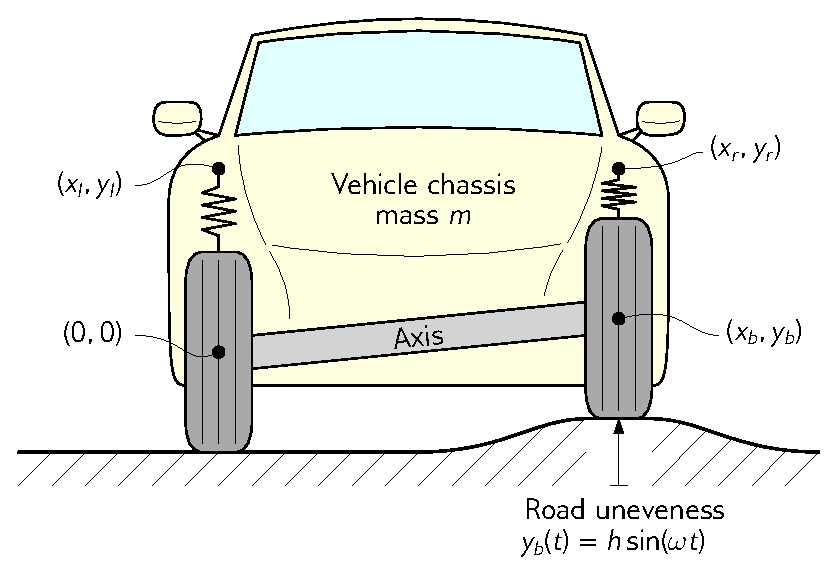
\includegraphics[width=\textwidth]{figures/car_axis.eps}
    \end{column}
  \end{columns}
  \centering{\scriptsize\begin{tabular}{cccc}
    \multicolumn{4}{c}{\textbf{Car-Axis (Index-3) -- \acs{LU} Factorization}} \\
    \toprule
    \textbf{Original \acsp{DAE}} & \multicolumn{3}{c}{$\mF = 108\cf + 131\cm + 56\ca$ \quad $\mh = 0$} \\
    \midrule
    \textbf{Reduction step} & $\mE$ & $\mg$ & $\ma$ \\
    \midrule
    Index-3 \acsp{DAE} & $12\cm$ & $94\cf + 145\cm + 54\ca$ & $14\cf + 16\cm + 10\ca$ \\
    Index-2 \acsp{DAE} & $12\cm$ & $94\cf + 145\cm + 54\ca$ & $26\cf + 45\cm + 15\ca$ \\
    Index-1 \acsp{DAE} & $12\cm$ & $94\cf + 145\cm + 54\ca$ & $136\cf + 4\cd + 261\cm + 95\ca$ \\
    Index-0 \acsp{DAE} & $1060\cf + 38\cd + 1901\cm + 717\ca$ & $431\cf + 8\cd + 842\cm + 268\ca$ & $0$ \\
    \midrule
    \rowcolor{mycolor5!25}
    \textbf{Reduced \acsp{DAE}} & \multicolumn{3}{c}{$\mF = 896\cf + 4\cd + 1202\cm + 546\ca$ \quad $\mh = 176\cf + 4\cd + 322\cm + 120\ca$} \\
    \bottomrule \\[0.05em]
    %
    \multicolumn{4}{c}{\textbf{Car-Axis (Index-3) -- \acs{FFLU} Factorization}} \\
    \toprule
    \textbf{Original \acsp{DAE}} & \multicolumn{3}{c}{$\mF = 108\cf + 131\cm + 56\ca$ \quad $\mh = 0$} \\
    \midrule
    \textbf{Reduction step} & $\mE$ & $\mg$ & $\ma$ \\
    \midrule
    Index-3 \acsp{DAE} & $0$ & $94\cf + 8\cd + 150\cm + 54\ca$ & $14\cf + 21\cm + 10\ca$ \\
    Index-2 \acsp{DAE} & $0$ & $94\cf + 8\cd + 154\cm + 54\ca$ & $26\cf + 1\cd + 44\cm + 15\ca$ \\
    Index-1 \acsp{DAE} & $0$ & $94\cf + 8\cd + 155\cm + 54\ca$ & $136\cf + 6\cd + 4\cd + 261\cm + 95\ca$ \\
    Index-0 \acsp{DAE} & $1066\cf + 55\cd + 1888\cm + 717\ca$ & $431\cf + 18\cd + 851\cm + 268\ca$ & $0$ \\
    \midrule
    \rowcolor{mycolor2!25}
    \textbf{Reduced \acsp{DAE}} & \multicolumn{3}{c}{$\mF = 1549\cf + 73\cd + 2765\cm + 1011\ca$ \quad $\mh = 176\cf + 7\cd + 326\cm + 120\ca$} \\
    \bottomrule
  \end{tabular}}
\end{frame}

\begin{frame}{Application Fields and Examples}{Expression Swell}
  \begin{columns}
    \centering
    \begin{column}[c]{0.7\textwidth}
      \hic{And when strong expression swell arise \dots}
    \end{column}
    \begin{column}[c]{0.22\textwidth}
      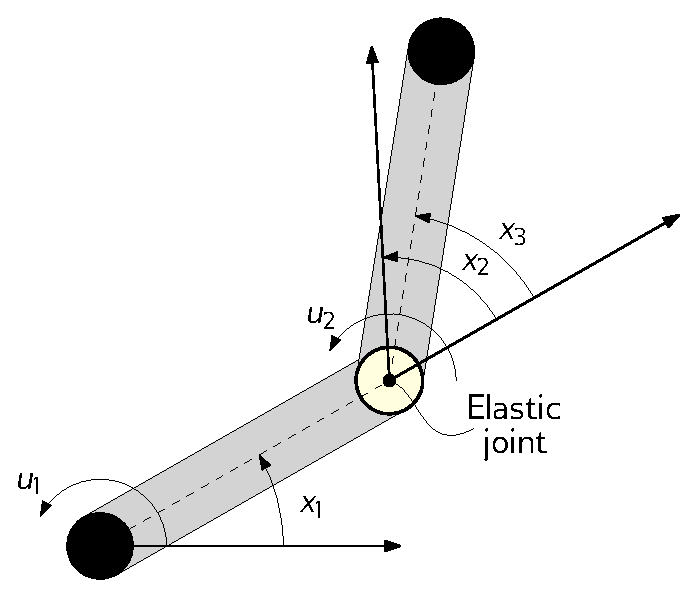
\includegraphics[width=\textwidth]{figures/robotic_arm.eps}
    \end{column}
  \end{columns}
  \hspace{-0.5em}
  \centering{\scriptsize\begin{tabular}{cccc}
    \multicolumn{4}{c}{\textbf{Robotic Arm (Index-5)}} \\
    \toprule
    \textbf{Original \acsp{DAE}} & \multicolumn{3}{c}{$\mF = 125\cf + 19\cd + 56\cm + 64\ca$ \quad $\mh = 0$} \\
    \midrule
    \textbf{Reduction step} & $\mE$ & $\mg$ & $\ma$ \\
    \midrule
    Index-5 \acsp{DAE} & $0$ & $66\cf + 3\cd + 50\cm + 35\ca$ & $16\cf + 12\ca$ \\
    Index-4 \acsp{DAE} & $0$ & $66\cf + 3\cd + 50\cm + 35\ca$ & $24\cf + 6\cm + 14\ca$ \\
    Index-3 \acsp{DAE} & $0$ & $66\cf + 3\cd + 50\cm + 35\ca$ & $162\cf + 2\cd + 138\cm + 114\ca$ \\
    Index-2 \acsp{DAE} & $14\cf + 2\cd + 6\cm + 6\ca$ & $372\cf + 4\cd + 375\cm + 253\ca$ & $972\cf + 1\cd + 1062\cm + 770\ca$ \\
    \rowcolor{mycolor2!25}
    Index-1 \acsp{DAE} & $14\cf + 2\cd + 6\cm + 6\ca$ & $372\cf + 4\cd + 375\cm + 253\ca$ & $\star (6.5\cf + 5.6\cm + 1.8\ca)\!\cdot\!10^{6} + 4\cd$ \\
    \rowcolor{mycolor2!25}
    Index-0 \acsp{DAE} & $\star (8.3\cf + 7.1\cm + 2.3\ca)\!\cdot\!10^{7} + 58\cd$ & $(2.4\cf + 2.0\cm + 0.9\ca)\!\cdot\!10^{6} + 8\cd$ & $0$ \\
    \midrule
    \rowcolor{mycolor2!25}
    \textbf{Reduced \acsp{DAE}} & \multicolumn{3}{c}{$\star \mF = (8.6\cf + 7.3\cm + 2.4\ca)\!\cdot\!10^{7} + 66\cd$ \quad $\star \mh = (6.5\cf + 5.6\cm + 1.8\ca)\!\cdot\!10^{6} + 7\cd$} \\
    \bottomrule
    \end{tabular}}
\end{frame}

\begin{frame}{Application Fields and Examples}{Expression Swell}
  \vspace{-2.0em}
  \hic{\dots hierarchical representation does the job}
  \vspace{-0.5em}
  \centering{\scriptsize\begin{tabular}{cccc}
    \multicolumn{4}{c}{\textbf{Robotic Arm (Index-5)}} \\
    \toprule
    \textbf{Original \acsp{DAE}} & \multicolumn{3}{c}{$\mFv = 125\cf + 19\cd + 56\cm + 64\ca$ \quad $\mhv = 0$ \quad $\mv = 0$} \\
    \midrule
    \textbf{Reduction step} & $\mEv$ & $\mgv$ & $\mav$ \\
    \midrule
    Index-5 \acsp{DAE} & $0$ & $66\cf + 3\cd + 50\cm + 35\ca$ & $16\cf + 12\ca$ \\
    Index-4 \acsp{DAE} & $0$ & $66\cf + 3\cd + 50\cm + 35\ca$ & $24\cf + 6\cm + 14\ca$ \\
    Index-3 \acsp{DAE} & $0$ & $66\cf + 3\cd + 50\cm + 35\ca$ & $162\cf + 2\cd + 138\cm + 114\ca$ \\
    Index-2 \acsp{DAE} & $14\cf + 2\cd + 6\cm + 6\ca$ & $66\cf + 1\cv + 3\cd + 51\cm + 35\ca$ & $1\cm + 1\cv$ \\
    \rowcolor{mycolor5!25}
    Index-1 \acsp{DAE} & $2\cv + 1\ca$ & $66\cf + 1\cv + 3\cd + 51\cm + 35\ca$ & \cellcolor{mycolor5!25}$9\cf + 4\cv + 2\cd + 8\cm + 5\ca$ \\
    \rowcolor{mycolor5!25}
    Index-0 \acsp{DAE} & $7\cv + 1\cd + 2\cm + 2\ca$ & \cellcolor{mycolor5!25}$66\cf + 2\cv + 3\cd + 52\cm + 35\ca$ & $0$ \\
    \midrule
    \rowcolor{mycolor5!25}
    \textbf{Reduced \acsp{DAE}} & \multicolumn{3}{c}{$\mFv = 90\cf + 9\cv + 4\cd + 63\cm + 48\ca$ \quad $\mhv = 202\cf + 5\cv + 4\cd + 141\cm + 130\ca$} \\
    \bottomrule \\[-0.65em]
  \end{tabular}}
  \begin{columns}
    \centering
    \begin{column}[c]{0.5\textwidth}
      \centering{\scriptsize\begin{tabular}{cc}
        \multicolumn{2}{c}{Hierarchical representation details (29 veils)} \\
        \toprule
        \textbf{Reduction step} & $\mv$ \\
        \midrule
        Index-5 \acsp{DAE} & $0$ \\
        Index-4 \acsp{DAE} & $0$ \\
        Index-3 \acsp{DAE} & $0$ \\
        Index-2 \acsp{DAE} & $1278\cf + 3\cv + 6\cd + 1319\cm + 918\ca$ \\
        \rowcolor{mycolor3!25}
        Index-1 \acsp{DAE} & $8401\cf + 20\cv + 24\cd + 9451\cm + 6095\ca$ \\
        \rowcolor{mycolor3!25}
        Index-0 \acsp{DAE} & $37010\cf + 558\cv + 56\cd + 45087\cm + 28665\ca$ \\
        \midrule
        \rowcolor{mycolor3!25}
        \textbf{Reduced \acsp{DAE}} & $\mv = 37010\cf + 558\cv + 56\cd + 45087\cm + 28665\ca$ \\
        \bottomrule
      \end{tabular}}
    \end{column}
    \hspace{1.0em}
    \begin{column}[c]{0.215\textwidth}
      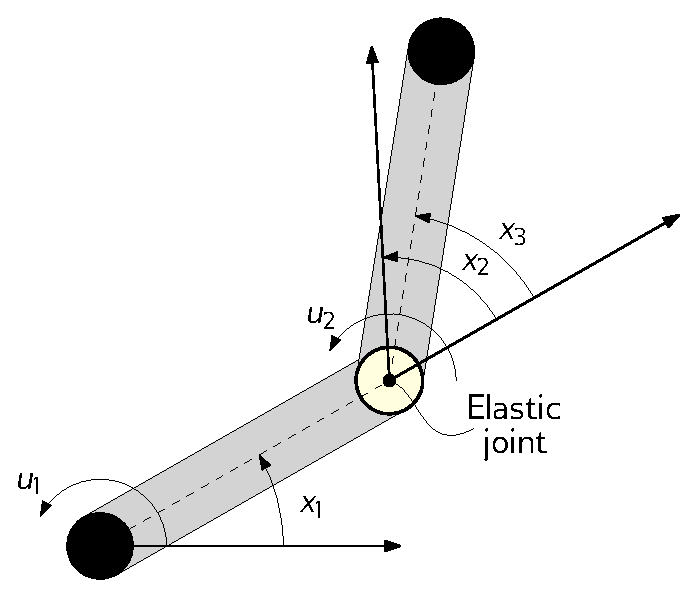
\includegraphics[width=\textwidth]{figures/robotic_arm.eps}
    \end{column}
  \end{columns}
\end{frame}

\begin{frame}{Application Fields and Examples}{Numerical Stability}
  \vspace{-2.0em}\begin{columns}
    \centering
    \begin{column}[c]{0.625\textwidth}
      \hic{Numerical stability is preserved}
    \end{column}
    \begin{column}[c]{0.3\textwidth}
      \vspace{1.5em}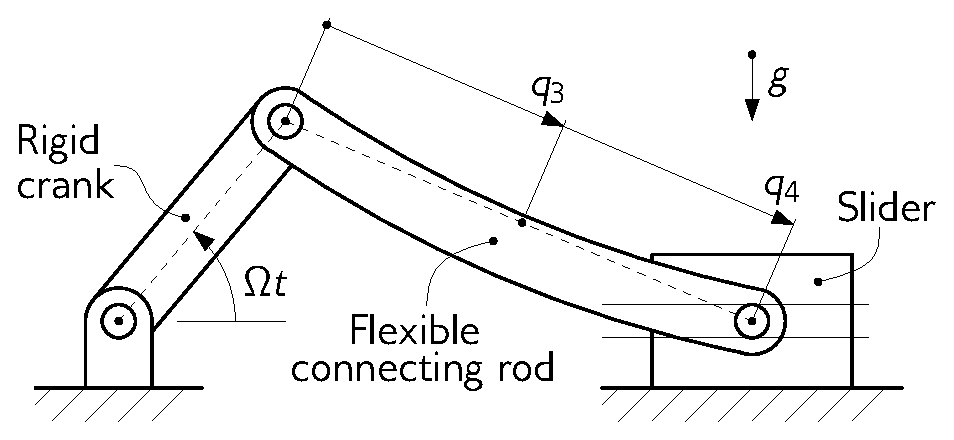
\includegraphics[width=\textwidth]{figures/flexible_slider_crank.eps}
    \end{column}
  \end{columns}
  \vspace{-1.5em}
  \small{\begin{tikzpicture}

\begin{axis}[%
  minor tick num=1,
  minor grid style={dashed, line width=.1pt, draw=gray!45},
  major grid style={line width=.2pt, draw=gray!60},
  width=5.25cm,
  height=4.0cm,
  at={(0.0in,0.0in)},
  scale only axis,
  xmin=0,
  xmax=0.1,
  xlabel style={font=\color{black}},
  xlabel={$t$ (\USI{\second})},
  ymin=-7.5e+01,
  ymax=2.5e+01,
  ylabel style={font=\color{black}},
  ylabel={$q_3$ (\USI{\micro\meter}) \quad -- \quad $q_4$ (\USI{\micro\meter})},
  xtick={0.0, 0.02, 0.04, 0.06, 0.08, 0.1},
  xticklabels={$0$, $0.02$, $0.04$, $0.06$, $0.08$, $0.1$},
  axis background/.style={fill=none},
  xmajorgrids,
  xminorgrids,
  ymajorgrids,
  yminorgrids
]

\addplot [color=mycolor1, line width=0.85pt, forget plot]
  table[row sep=crcr]{%
0	10.3339863\\
0.0001	10.3311196150886\\
0.0002	10.3245617197689\\
0.0003	10.3171164036229\\
0.0004	10.3104069768556\\
0.0005	10.3038779267391\\
0.0006	10.2954986667631\\
0.0007	10.2835713824365\\
0.0008	10.2681429047285\\
0.0009	10.2508564648278\\
0.001	10.2333745243603\\
0.0011	10.2156894451652\\
0.0012	10.1957369580273\\
0.0013	10.1706578652081\\
0.0014	10.1386982946831\\
0.0015	10.1002147093181\\
0.0016	10.0569875766454\\
0.0017	10.0104381380362\\
0.0018	9.96024028902651\\
0.0019	9.90448597891853\\
0.002	9.84127441309934\\
0.0021	9.77041492290039\\
0.0022	9.6938327760751\\
0.0023	9.61432839185016\\
0.0024	9.53368911583447\\
0.0025	9.45167930109935\\
0.0026	9.36670724908208\\
0.0027	9.27758672090818\\
0.0028	9.18491279559687\\
0.0029	9.09089428074181\\
0.003	8.99776048727888\\
0.0031	8.90603866123845\\
0.0032	8.81411098380601\\
0.0033	8.71941546844372\\
0.0034	8.62031267999506\\
0.0035	8.51710235414694\\
0.0036	8.41138040534289\\
0.0037	8.30429495191616\\
0.0038	8.1951654707874\\
0.0039	8.08162966793374\\
0.004	7.96122601537002\\
0.0041	7.8331387455824\\
0.0042	7.69869509387642\\
0.0043	7.5602224532141\\
0.0044	7.41920983901015\\
0.0045	7.27527822636761\\
0.0046	7.12679113604333\\
0.0047	6.9725847155947\\
0.0048	6.81337455856543\\
0.0049	6.65165896662697\\
0.005	6.49016835015624\\
0.0051	6.33009972602237\\
0.0052	6.17055106195062\\
0.0053	6.00959076636354\\
0.0054	5.84606590255815\\
0.0055	5.68065760331278\\
0.0056	5.51531790251052\\
0.0057	5.35155437618704\\
0.0058	5.18897741331495\\
0.0059	5.02531544537955\\
0.006	4.85790907934953\\
0.0061	4.68549229693033\\
0.0062	4.50883879118218\\
0.0063	4.3297795224345\\
0.0064	4.14942438767133\\
0.0065	3.96706408491275\\
0.0066	3.78066536440588\\
0.0067	3.58856559918374\\
0.0068	3.39098804956862\\
0.0069	3.19013907259766\\
0.007	2.98879712254803\\
0.0071	2.78852412569575\\
0.0072	2.58892956366881\\
0.0073	2.38855480554123\\
0.0074	2.18662440211555\\
0.0075	1.98420742065679\\
0.0076	1.78381627438183\\
0.0077	1.58774660353514\\
0.0078	1.39649065029544\\
0.0079	1.20850231447998\\
0.008	1.021500309492\\
0.0081	0.834254630618885\\
0.0082	0.647418451891882\\
0.0083	0.462751496417193\\
0.0084	0.281393039675802\\
0.0085	0.102616895337795\\
0.0086	-0.0758905237454403\\
0.0087	-0.256425493774236\\
0.0088	-0.439610683468974\\
0.0089	-0.624007401257683\\
0.009	-0.807292659051989\\
0.0091	-0.988035718582095\\
0.0092	-1.16663193706729\\
0.0093	-1.34464454860787\\
0.0094	-1.52310398409514\\
0.0095	-1.70116556203179\\
0.0096	-1.87624017469812\\
0.0097	-2.04552166501945\\
0.0098	-2.20770440631777\\
0.0099	-2.36353054157776\\
0.01	-2.51475241815181\\
0.0101	-2.66237499300558\\
0.0102	-2.80561935716482\\
0.0103	-2.9424561156526\\
0.0104	-3.07127715568154\\
0.0105	-3.1923440875958\\
0.0106	-3.30782517652131\\
0.0107	-3.42036949899305\\
0.0108	-3.53134674652527\\
0.0109	-3.64014843536441\\
0.011	-3.74508508544087\\
0.0111	-3.84512192567915\\
0.0112	-3.94101938329261\\
0.0113	-4.03493173352347\\
0.0114	-4.12877301641456\\
0.0115	-4.22266595730403\\
0.0116	-4.31473086851303\\
0.0117	-4.4023940099515\\
0.0118	-4.48417092015367\\
0.0119	-4.56050131599256\\
0.012	-4.63298551465216\\
0.0121	-4.70267131734079\\
0.0122	-4.76881169903016\\
0.0123	-4.8291313527408\\
0.0124	-4.88141336508655\\
0.0125	-4.92514081408042\\
0.0126	-4.96187590069781\\
0.0127	-4.99407520610907\\
0.0128	-5.02330076296352\\
0.0129	-5.04926979185454\\
0.013	-5.07049847372054\\
0.0131	-5.08599449847881\\
0.0132	-5.09659566857724\\
0.0133	-5.10483523162924\\
0.0134	-5.11341029004043\\
0.0135	-5.12346688991033\\
0.0136	-5.13406928805226\\
0.0137	-5.14326456077883\\
0.0138	-5.14986309977861\\
0.0139	-5.15447985659477\\
0.014	-5.15898959917901\\
0.0141	-5.16484794467534\\
0.0142	-5.17166167959487\\
0.0143	-5.1771967930575\\
0.0144	-5.17884733578219\\
0.0145	-5.17540037521583\\
0.0146	-5.16769001044505\\
0.0147	-5.15763582488689\\
0.0148	-5.14647442115773\\
0.0149	-5.1336464248081\\
0.015	-5.11726131066196\\
0.0151	-5.09576773721615\\
0.0152	-5.0694639898422\\
0.0153	-5.04060376737777\\
0.0154	-5.01199094147028\\
0.0155	-4.9851852739383\\
0.0156	-4.95975606051857\\
0.0157	-4.93416343675031\\
0.0158	-4.9075166540072\\
0.0159	-4.88074235933989\\
0.016	-4.85618076315632\\
0.0161	-4.8359186533506\\
0.0162	-4.82020974983484\\
0.0163	-4.80727119795095\\
0.0164	-4.79462809273771\\
0.0165	-4.7809182819658\\
0.0166	-4.76669857230987\\
0.0167	-4.7536160243138\\
0.0168	-4.74265160910961\\
0.0169	-4.73290706901385\\
0.017	-4.721962051097\\
0.0171	-4.70753950170349\\
0.0172	-4.68913935437731\\
0.0173	-4.668318978249\\
0.0174	-4.64740070785668\\
0.0175	-4.62766963208495\\
0.0176	-4.6085360809703\\
0.0177	-4.5883383960719\\
0.0178	-4.56610762876581\\
0.0179	-4.54281896489834\\
0.018	-4.5210710030465\\
0.0181	-4.50342329344536\\
0.0182	-4.49072614997568\\
0.0183	-4.48178692080505\\
0.0184	-4.47462364668836\\
0.0185	-4.46825788448462\\
0.0186	-4.46356156201805\\
0.0187	-4.46245811709944\\
0.0188	-4.46614039830165\\
0.0189	-4.47378569099144\\
0.019	-4.48284727452615\\
0.0191	-4.49071039055806\\
0.0192	-4.49638059339699\\
0.0193	-4.5008464311069\\
0.0194	-4.50584871103858\\
0.0195	-4.51209817896331\\
0.0196	-4.51843371512674\\
0.0197	-4.52263263314461\\
0.0198	-4.52321594650987\\
0.0199	-4.52076267754517\\
0.02	-4.51764261717612\\
0.0201	-4.51637205640813\\
0.0202	-4.51792537803075\\
0.0203	-4.52136701031405\\
0.0204	-4.52507665953145\\
0.0205	-4.52852566650562\\
0.0206	-4.53310831751181\\
0.0207	-4.54131388970471\\
0.0208	-4.55489859098831\\
0.0209	-4.57354840261475\\
0.021	-4.59512718831383\\
0.0211	-4.61730544219107\\
0.0212	-4.63923447880082\\
0.0213	-4.66190100397259\\
0.0214	-4.68689230178145\\
0.0215	-4.71461881756831\\
0.0216	-4.74349203554276\\
0.0217	-4.77076856335446\\
0.0218	-4.79439536166876\\
0.0219	-4.81436156603868\\
0.022	-4.83246415704731\\
0.0221	-4.85069672372175\\
0.0222	-4.86959880447852\\
0.0223	-4.88792727059464\\
0.0224	-4.9039117698283\\
0.0225	-4.91704131053785\\
0.0226	-4.9288842902102\\
0.0227	-4.94223702076221\\
0.0228	-4.95927206618745\\
0.0229	-4.9801819719807\\
0.023	-5.00340631683248\\
0.0231	-5.02722703701155\\
0.0232	-5.0513936951882\\
0.0233	-5.07742303950679\\
0.0234	-5.10731920828198\\
0.0235	-5.14177221189617\\
0.0236	-5.17933058549639\\
0.0237	-5.2172477276626\\
0.0238	-5.25332732934597\\
0.0239	-5.28727450658094\\
0.024	-5.32047029193894\\
0.0241	-5.35438814195307\\
0.0242	-5.38898884920336\\
0.0243	-5.42244352901204\\
0.0244	-5.45243329756245\\
0.0245	-5.47796759542791\\
0.0246	-5.50022833065047\\
0.0247	-5.52174223055563\\
0.0248	-5.54455334290057\\
0.0249	-5.56888330747381\\
0.025	-5.59335795673689\\
0.0251	-5.6165834949334\\
0.0252	-5.63874182622066\\
0.0253	-5.66185955108114\\
0.0254	-5.68850001032962\\
0.0255	-5.71992996462858\\
0.0256	-5.75524976410284\\
0.0257	-5.7921889006929\\
0.0258	-5.82890605160955\\
0.0259	-5.86531536138516\\
0.026	-5.90285987193058\\
0.0261	-5.94293838855831\\
0.0262	-5.9853051173831\\
0.0263	-6.02778682388832\\
0.0264	-6.06758023072598\\
0.0265	-6.10309346325524\\
0.0266	-6.13484721314537\\
0.0267	-6.16472114435211\\
0.0268	-6.19418517614026\\
0.0269	-6.22298111557746\\
0.027	-6.24934074191453\\
0.0271	-6.27155555114423\\
0.0272	-6.2895960124179\\
0.0273	-6.30543176530952\\
0.0274	-6.32176579185029\\
0.0275	-6.34019309175085\\
0.0276	-6.36026339290562\\
0.0277	-6.38018459750964\\
0.0278	-6.39855982072157\\
0.0279	-6.41570846946887\\
0.028	-6.43347035720703\\
0.0281	-6.45364360077918\\
0.0282	-6.47633450805699\\
0.0283	-6.49957674405677\\
0.0284	-6.52054386728974\\
0.0285	-6.5373810386908\\
0.0286	-6.55018132900677\\
0.0287	-6.56033778992466\\
0.0288	-6.56883470345961\\
0.0289	-6.57490881738867\\
0.029	-6.57620471802127\\
0.0291	-6.57032038646171\\
0.0292	-6.55649562429818\\
0.0293	-6.53607298886784\\
0.0294	-6.51135804563761\\
0.0295	-6.48380690128416\\
0.0296	-6.45301044312064\\
0.0297	-6.41728520805357\\
0.0298	-6.3753612526304\\
0.0299	-6.32775743042999\\
0.03	-6.27668943924917\\
0.0301	-6.22455648612582\\
0.0302	-6.1722165558508\\
0.0303	-6.11843676588342\\
0.0304	-6.06095051113264\\
0.0305	-5.99824753248117\\
0.0306	-5.93063289998415\\
0.0307	-5.85969710966292\\
0.0308	-5.78664551662943\\
0.0309	-5.71087353182742\\
0.031	-5.62997795443937\\
0.0311	-5.54122488429614\\
0.0312	-5.44330650463144\\
0.0313	-5.33698279397429\\
0.0314	-5.22411246219124\\
0.0315	-5.10588822788927\\
0.0316	-4.98173476973517\\
0.0317	-4.84977867353595\\
0.0318	-4.70850756328079\\
0.0319	-4.55825621029365\\
0.032	-4.40129109640894\\
0.0321	-4.24040294202858\\
0.0322	-4.07713010170042\\
0.0323	-3.91103381159303\\
0.0324	-3.74058573969763\\
0.0325	-3.56491200915067\\
0.0326	-3.38494097302348\\
0.0327	-3.20299378591497\\
0.0328	-3.02113543787662\\
0.0329	-2.83962442428611\\
0.033	-2.65672706392258\\
0.0331	-2.4700556203672\\
0.0332	-2.27835150101198\\
0.0333	-2.0822772154136\\
0.0334	-1.88359582469537\\
0.0335	-1.68343819057665\\
0.0336	-1.48110579124797\\
0.0337	-1.27441844355685\\
0.0338	-1.06134984757682\\
0.0339	-0.841635127489715\\
0.034	-0.61705025321673\\
0.0341	-0.390141811939229\\
0.0342	-0.162445656739331\\
0.0343	0.066356258011586\\
0.0344	0.297666506863667\\
0.0345	0.532242578175686\\
0.0346	0.768951160705845\\
0.0347	1.00505809342046\\
0.0348	1.23784925116479\\
0.0349	1.46628571598825\\
0.035	1.69136433786655\\
0.0351	1.91490991493147\\
0.0352	2.13780414040991\\
0.0353	2.35911118891853\\
0.0354	2.57681712640126\\
0.0355	2.78956877320253\\
0.0356	2.99796960219784\\
0.0357	3.20434620817418\\
0.0358	3.41114838326643\\
0.0359	3.61926451123599\\
0.036	3.82760351889213\\
0.0361	4.03425689024325\\
0.0362	4.23826027914187\\
0.0363	4.44048641512225\\
0.0364	4.64292051224807\\
0.0365	4.84690579264847\\
0.0366	5.05180182082301\\
0.0367	5.25516822306058\\
0.0368	5.45434069954808\\
0.0369	5.64812782432628\\
0.037	5.83726179500025\\
0.0371	6.02326308946775\\
0.0372	6.206684101444\\
0.0373	6.3862067155284\\
0.0374	6.55936329212691\\
0.0375	6.724309461322\\
0.0376	6.88120413056961\\
0.0377	7.03206670916966\\
0.0378	7.17922623659191\\
0.0379	7.32362828601827\\
0.038	7.46437567451654\\
0.0381	7.59985717724331\\
0.0382	7.72950596294462\\
0.0383	7.85470771703094\\
0.0384	7.97807797833056\\
0.0385	8.10167344228297\\
0.0386	8.22558454398908\\
0.0387	8.34804860156067\\
0.0388	8.46697702467076\\
0.0389	8.58163253688024\\
0.039	8.69307681392724\\
0.0391	8.80303056285972\\
0.0392	8.91210439072389\\
0.0393	9.01888396946826\\
0.0394	9.12065318900546\\
0.0395	9.21519064605418\\
0.0396	9.3021896811889\\
0.0397	9.38316046087114\\
0.0398	9.45992043575801\\
0.0399	9.53293799933514\\
0.04	9.6009079993893\\
0.0401	9.66191337030844\\
0.0402	9.71521015362202\\
0.0403	9.76215073044548\\
0.0404	9.80546386378914\\
0.0405	9.84745997205091\\
0.0406	9.88861256045679\\
0.0407	9.92765406521858\\
0.0408	9.96307477914958\\
0.0409	9.99475823030034\\
0.041	10.0243784809064\\
0.0411	10.0542128172801\\
0.0412	10.0853382766466\\
0.0413	10.1166967993911\\
0.0414	10.1458051467836\\
0.0415	10.1705366130892\\
0.0416	10.1905247576923\\
0.0417	10.2070575708314\\
0.0418	10.2215802115031\\
0.0419	10.234074012719\\
0.042	10.2426804757322\\
0.0421	10.2449087622648\\
0.0422	10.2394543519912\\
0.0423	10.2271467073534\\
0.0424	10.2102553357336\\
0.0425	10.1907294351456\\
0.0426	10.1688167307873\\
0.0427	10.143185445054\\
0.0428	10.1124263348357\\
0.0429	10.0766686626977\\
0.043	10.0379473535554\\
0.0431	9.99898733309802\\
0.0432	9.96137635893018\\
0.0433	9.92460360590627\\
0.0434	9.88673162312847\\
0.0435	9.84612963813366\\
0.0436	9.80283028181973\\
0.0437	9.75839172680218\\
0.0438	9.71438752411434\\
0.0439	9.67078413570623\\
0.044	9.6255642306133\\
0.0441	9.57593238035008\\
0.0442	9.52014062024086\\
0.0443	9.45846363915457\\
0.0444	9.39255363753663\\
0.0445	9.32373543752115\\
0.0446	9.25166820785352\\
0.0447	9.17449028388959\\
0.0448	9.09033506230803\\
0.0449	8.99897066531554\\
0.045	8.90220748919512\\
0.0451	8.80272401648401\\
0.0452	8.70225439038581\\
0.0453	8.60059906876015\\
0.0454	8.4962388428698\\
0.0455	8.38801408942678\\
0.0456	8.27645876357576\\
0.0457	8.1636673795452\\
0.0458	8.05178379251047\\
0.0459	7.94133785333766\\
0.046	7.83078690902363\\
0.0461	7.71763769905259\\
0.0462	7.60023654033226\\
0.0463	7.47877713714071\\
0.0464	7.35472515855505\\
0.0465	7.2291617628857\\
0.0466	7.10143570406466\\
0.0467	6.9692595468593\\
0.0468	6.83020014658037\\
0.0469	6.6833690177846\\
0.047	6.52995110450201\\
0.0471	6.37215579008652\\
0.0472	6.21145684425298\\
0.0473	6.04755945073318\\
0.0474	5.87892754121665\\
0.0475	5.70442077106632\\
0.0476	5.52467841507028\\
0.0477	5.34209174200825\\
0.0478	5.15935815548985\\
0.0479	4.97776757149485\\
0.048	4.79658983439438\\
0.0481	4.61403524834108\\
0.0482	4.42898207390264\\
0.0483	4.24204783851753\\
0.0484	4.05512659426501\\
0.0485	3.86977434945418\\
0.0486	3.68577096118579\\
0.0487	3.501048257658\\
0.0488	3.31306566670159\\
0.0489	3.12054030727581\\
0.049	2.92415406391973\\
0.0491	2.72569506098714\\
0.0492	2.5263635944542\\
0.0493	2.32564704470448\\
0.0494	2.12169759351453\\
0.0495	1.91291608308409\\
0.0496	1.69945726772132\\
0.0497	1.48342908885325\\
0.0498	1.26761341528112\\
0.0499	1.05372978314101\\
0.05	0.841627508172789\\
0.0501	0.630031600213549\\
0.0502	0.418203400215481\\
0.0503	0.207135174263521\\
0.0504	-0.000719943598841945\\
0.0505	-0.202987336961387\\
0.0506	-0.398948757701495\\
0.0507	-0.589890750321688\\
0.0508	-0.777946292169766\\
0.0509	-0.964366265846955\\
0.051	-1.14861080673157\\
0.0511	-1.32897742902185\\
0.0512	-1.5042306703516\\
0.0513	-1.67488275052952\\
0.0514	-1.84305685250051\\
0.0515	-2.01101444216561\\
0.0516	-2.17951301340831\\
0.0517	-2.34730164306798\\
0.0518	-2.51214507438895\\
0.0519	-2.67253573840285\\
0.052	-2.82870430949718\\
0.0521	-2.9821165874505\\
0.0522	-3.13387891454664\\
0.0523	-3.28336522948846\\
0.0524	-3.42820432629087\\
0.0525	-3.56566734253918\\
0.0526	-3.69436278335047\\
0.0527	-3.81489687070969\\
0.0528	-3.92899267079096\\
0.0529	-4.0378054351055\\
0.053	-4.14081647964082\\
0.0531	-4.23621170327113\\
0.0532	-4.32243974579152\\
0.0533	-4.39968052412193\\
0.0534	-4.47001943704383\\
0.0535	-4.53616443879178\\
0.0536	-4.59971886067699\\
0.0537	-4.66037978938796\\
0.0538	-4.7166804727018\\
0.0539	-4.76764422847941\\
0.054	-4.81398069389739\\
0.0541	-4.85783052942904\\
0.0542	-4.90124801416431\\
0.0543	-4.94464260931866\\
0.0544	-4.9864428271463\\
0.0545	-5.02426282719305\\
0.0546	-5.05664026143061\\
0.0547	-5.08395605314823\\
0.0548	-5.10781513642706\\
0.0549	-5.12941986991266\\
0.055	-5.1482878009628\\
0.0551	-5.16238588291148\\
0.0552	-5.16959997306709\\
0.0553	-5.16936790450232\\
0.0554	-5.16316366549471\\
0.0555	-5.15344550606949\\
0.0556	-5.1419216108879\\
0.0557	-5.12853489410497\\
0.0558	-5.11197713161313\\
0.0559	-5.09129213303181\\
0.056	-5.06723548999874\\
0.0561	-5.04225208381079\\
0.0562	-5.01905625115109\\
0.0563	-4.99893934039102\\
0.0564	-4.98115635257605\\
0.0565	-4.96387064906074\\
0.0566	-4.94587266423232\\
0.0567	-4.92766417230222\\
0.0568	-4.9110238737073\\
0.0569	-4.8974165580732\\
0.057	-4.88656014470469\\
0.0571	-4.87634415555903\\
0.0572	-4.86419588465755\\
0.0573	-4.84881094689446\\
0.0574	-4.8308664767592\\
0.0575	-4.81216342188714\\
0.0576	-4.793924234057\\
0.0577	-4.77565831907687\\
0.0578	-4.75553805331843\\
0.0579	-4.73198558420225\\
0.058	-4.70517102643832\\
0.0581	-4.67718526525833\\
0.0582	-4.65072657763435\\
0.0583	-4.62735081655164\\
0.0584	-4.606689064331\\
0.0585	-4.58724312031325\\
0.0586	-4.56807648493197\\
0.0587	-4.54998546389904\\
0.0588	-4.53516348081292\\
0.0589	-4.52561193846294\\
0.059	-4.52158659771932\\
0.0591	-4.52134892347517\\
0.0592	-4.52243093460716\\
0.0593	-4.52338836019302\\
0.0594	-4.52462238901613\\
0.0595	-4.52761974204495\\
0.0596	-4.53326356892978\\
0.0597	-4.54063402987574\\
0.0598	-4.54731672467698\\
0.0599	-4.55099697465011\\
0.06	-4.55105668806915\\
0.0601	-4.54888119810798\\
0.0602	-4.54663558949825\\
0.0603	-4.54552025340097\\
0.0604	-4.544936153865\\
0.0605	-4.54323492906948\\
0.0606	-4.53941813909905\\
0.0607	-4.53436232809493\\
0.0608	-4.53053145913068\\
0.0609	-4.53038050024184\\
0.061	-4.5347318012423\\
0.0611	-4.54243161002572\\
0.0612	-4.55154517599664\\
0.0613	-4.56108795498996\\
0.0614	-4.57185560753161\\
0.0615	-4.58566530874528\\
0.0616	-4.60363801492762\\
0.0617	-4.62495020260806\\
0.0618	-4.64710475410196\\
0.0619	-4.6675249080736\\
0.062	-4.68518841500088\\
0.0621	-4.70098709339474\\
0.0622	-4.71654684833426\\
0.0623	-4.73250992703162\\
0.0624	-4.7477204322105\\
0.0625	-4.76000343766834\\
0.0626	-4.76790636605449\\
0.0627	-4.77196902698109\\
0.0628	-4.77446852020569\\
0.0629	-4.77783490747302\\
0.063	-4.78302307458902\\
0.0631	-4.78915706308945\\
0.0632	-4.79470989195219\\
0.0633	-4.79921348157325\\
0.0634	-4.80405640424342\\
0.0635	-4.81168248752878\\
0.0636	-4.82382757773678\\
0.0637	-4.84023198703341\\
0.0638	-4.85888141727405\\
0.0639	-4.87757630343942\\
0.064	-4.89554179662199\\
0.0641	-4.91376504888885\\
0.0642	-4.93380360221411\\
0.0643	-4.95607562601303\\
0.0644	-4.97907361642905\\
0.0645	-5.0001822746158\\
0.0646	-5.0174565804138\\
0.0647	-5.03092081601986\\
0.0648	-5.04233975635074\\
0.0649	-5.0536673111407\\
0.065	-5.06546111999977\\
0.0651	-5.07657090161051\\
0.0652	-5.08534879437862\\
0.0653	-5.09136657129064\\
0.0654	-5.09620020178656\\
0.0655	-5.10260689855264\\
0.0656	-5.11274261941789\\
0.0657	-5.12685798035459\\
0.0658	-5.14351660401431\\
0.0659	-5.16112753066122\\
0.066	-5.17950535355674\\
0.0661	-5.20015640926876\\
0.0662	-5.22504806966257\\
0.0663	-5.25487696133838\\
0.0664	-5.288272603431\\
0.0665	-5.32260893676955\\
0.0666	-5.35577749976549\\
0.0667	-5.38748908440374\\
0.0668	-5.41906302344088\\
0.0669	-5.45191038846098\\
0.067	-5.48599135016013\\
0.0671	-5.51954365470329\\
0.0672	-5.55032615985655\\
0.0673	-5.57736701918869\\
0.0674	-5.60178359757296\\
0.0675	-5.62599793014159\\
0.0676	-5.65198407636667\\
0.0677	-5.67997210046316\\
0.0678	-5.70865019830296\\
0.0679	-5.73666869696451\\
0.068	-5.76417656433435\\
0.0681	-5.79309502301488\\
0.0682	-5.82587402119878\\
0.0683	-5.86372839950403\\
0.0684	-5.90578286731224\\
0.0685	-5.94981381743939\\
0.0686	-5.99397145501627\\
0.0687	-6.0380694880857\\
0.0688	-6.08339440922286\\
0.0689	-6.13121052978851\\
0.069	-6.18121371389139\\
0.0691	-6.23123207317545\\
0.0692	-6.27844963465654\\
0.0693	-6.32117931368539\\
0.0694	-6.35975999032674\\
0.0695	-6.39586852135178\\
0.0696	-6.43083252791948\\
0.0697	-6.46434146391836\\
0.0698	-6.4946175000944\\
0.0699	-6.51990169649139\\
0.07	-6.54002502154986\\
0.0701	-6.55675824587398\\
0.0702	-6.57263059491393\\
0.0703	-6.58915747290856\\
0.0704	-6.60589838409821\\
0.0705	-6.62108482758519\\
0.0706	-6.63327384256958\\
0.0707	-6.6426478861672\\
0.0708	-6.65087841765064\\
0.0709	-6.65965427858664\\
0.071	-6.66907649302486\\
0.0711	-6.67723762087374\\
0.0712	-6.68134160121539\\
0.0713	-6.67946685388559\\
0.0714	-6.67155596345462\\
0.0715	-6.65885305848444\\
0.0716	-6.64228198929049\\
0.0717	-6.62112390842453\\
0.0718	-6.59310483214507\\
0.0719	-6.55584621735553\\
0.072	-6.50851170898791\\
0.0721	-6.45231649457288\\
0.0722	-6.38948799591168\\
0.0723	-6.32152399871548\\
0.0724	-6.24815984082319\\
0.0725	-6.1678690724938\\
0.0726	-6.07946308039334\\
0.0727	-5.98345368502359\\
0.0728	-5.88203500446775\\
0.0729	-5.77766933759655\\
0.073	-5.67140430197208\\
0.0731	-5.5622717714794\\
0.0732	-5.44824107617875\\
0.0733	-5.32793658729904\\
0.0734	-5.20171371964253\\
0.0735	-5.07121988536893\\
0.0736	-4.93781227335568\\
0.0737	-4.80114480250818\\
0.0738	-4.65910374233242\\
0.0739	-4.50917357735095\\
0.074	-4.35014821332419\\
0.0741	-4.18282016969154\\
0.0742	-4.00911270552607\\
0.0743	-3.83038727445691\\
0.0744	-3.64632630633286\\
0.0745	-3.4553140195401\\
0.0746	-3.25600600385689\\
0.0747	-3.04879863468552\\
0.0748	-2.83598314528665\\
0.0749	-2.62043700033307\\
0.075	-2.40389522043729\\
0.0751	-2.18618425903706\\
0.0752	-1.96601290004276\\
0.0753	-1.74264231990436\\
0.0754	-1.51704096405187\\
0.0755	-1.2915552770301\\
0.0756	-1.06834706885659\\
0.0757	-0.847864766296018\\
0.0758	-0.628596781911942\\
0.0759	-0.408314999017268\\
0.076	-0.185804837001012\\
0.0761	0.0383135696178197\\
0.0762	0.262319868689245\\
0.0763	0.485053543017849\\
0.0764	0.707109619366786\\
0.0765	0.930560274460342\\
0.0766	1.15740223419548\\
0.0767	1.38797860807644\\
0.0768	1.62065184861735\\
0.0769	1.85298748504773\\
0.077	2.08347824515628\\
0.0771	2.31240274879681\\
0.0772	2.54112936758173\\
0.0773	2.77045719433748\\
0.0774	2.99938146421176\\
0.0775	3.22532684526809\\
0.0776	3.44568956937234\\
0.0777	3.65945422890351\\
0.0778	3.86758588721347\\
0.0779	4.07189768922222\\
0.078	4.2733391401149\\
0.0781	4.47111893765462\\
0.0782	4.66338344934998\\
0.0783	4.84888615047239\\
0.0784	5.02826101113298\\
0.0785	5.20383071456424\\
0.0786	5.37807901155749\\
0.0787	5.55201151657915\\
0.0788	5.7247206565841\\
0.0789	5.89448224609355\\
0.079	6.06045496247251\\
0.0791	6.22356268110408\\
0.0792	6.38581774730924\\
0.0793	6.54863342012588\\
0.0794	6.71151418732351\\
0.0795	6.87221069970843\\
0.0796	7.0282287321296\\
0.0797	7.17847334627857\\
0.0798	7.3237024464283\\
0.0799	7.46544671594822\\
0.08	7.60431665760388\\
0.0801	7.73912131338368\\
0.0802	7.86755168775335\\
0.0803	7.98788769239038\\
0.0804	8.10033697611843\\
0.0805	8.2069089123174\\
0.0806	8.30992545863059\\
0.0807	8.41038583886626\\
0.0808	8.507515218385\\
0.0809	8.5998454341029\\
0.081	8.68690806933315\\
0.0811	8.77011229479171\\
0.0812	8.85205124219787\\
0.0813	8.93477807770148\\
0.0814	9.01844647747723\\
0.0815	9.10141547987798\\
0.0816	9.18171808933493\\
0.0817	9.25867619046031\\
0.0818	9.33333206251793\\
0.0819	9.40735127754518\\
0.082	9.48132038329237\\
0.0821	9.5538683533119\\
0.0822	9.62236569206529\\
0.0823	9.68465595986634\\
0.0824	9.74042307267693\\
0.0825	9.79109652066719\\
0.0826	9.83839915080332\\
0.0827	9.88275631830415\\
0.0828	9.92289209760259\\
0.0829	9.95695033741296\\
0.083	9.98421160893799\\
0.0831	10.0059774193279\\
0.0832	10.0248730962944\\
0.0833	10.0431195373565\\
0.0834	10.0611701586551\\
0.0835	10.0778052436167\\
0.0836	10.0915730587698\\
0.0837	10.1023583288482\\
0.0838	10.1117584376096\\
0.0839	10.1219378785886\\
0.084	10.1338942207146\\
0.0841	10.1465619659225\\
0.0842	10.1574973904903\\
0.0843	10.1645915080847\\
0.0844	10.1674182415564\\
0.0845	10.1671325656023\\
0.0846	10.1650337663566\\
0.0847	10.1610113849621\\
0.0848	10.1531870312323\\
0.0849	10.1390761884729\\
0.085	10.1173367506227\\
0.0851	10.0886821106451\\
0.0852	10.0552186709741\\
0.0853	10.0187580130602\\
0.0854	9.97948955462691\\
0.0855	9.93609317724946\\
0.0856	9.88717722284392\\
0.0857	9.8328302942592\\
0.0858	9.77497891954026\\
0.0859	9.71622569099335\\
0.086	9.65809393982642\\
0.0861	9.60009504584279\\
0.0862	9.54036074116669\\
0.0863	9.47730085066244\\
0.0864	9.41091172020939\\
0.0865	9.34265781699944\\
0.0866	9.27403195087024\\
0.0867	9.20499375454788\\
0.0868	9.13359164749665\\
0.0869	9.05710480782053\\
0.087	8.97379600465232\\
0.0871	8.88386703643483\\
0.0872	8.78886455629424\\
0.0873	8.69005459752549\\
0.0874	8.58712516125825\\
0.0875	8.4782985354589\\
0.0876	8.36176893210692\\
0.0877	8.23728545511734\\
0.0878	8.10657449161599\\
0.0879	7.97224139543497\\
0.088	7.83603185953579\\
0.0881	7.69785165759121\\
0.0882	7.55631648259121\\
0.0883	7.41034759182424\\
0.0884	7.26047408632524\\
0.0885	7.10874814836632\\
0.0886	6.95732199007817\\
0.0887	6.80683730235968\\
0.0888	6.65593739286605\\
0.0889	6.5022999552734\\
0.089	6.34435233706101\\
0.0891	6.18228215916459\\
0.0892	6.01754104306177\\
0.0893	5.85127710526046\\
0.0894	5.68300953470126\\
0.0895	5.51065956416503\\
0.0896	5.3319412488151\\
0.0897	5.14600175792427\\
0.0898	4.95399371290769\\
0.0899	4.75812895498337\\
0.09	4.55999493434016\\
0.0901	4.35950671405338\\
0.0902	4.15533875045158\\
0.0903	3.94646524619099\\
0.0904	3.73352852686325\\
0.0905	3.51889231472074\\
0.0906	3.30530712542842\\
0.0907	3.09424480626792\\
0.0908	2.88522849076813\\
0.0909	2.67667547091841\\
0.091	2.46754385654375\\
0.0911	2.2584278967619\\
0.0912	2.05120529290754\\
0.0913	1.8475271304702\\
0.0914	1.6473898286792\\
0.0915	1.44896741584203\\
0.0916	1.24986256996394\\
0.0917	1.04878628020403\\
0.0918	0.846331668641687\\
0.0919	0.64424545904114\\
0.092	0.443819583453749\\
0.0921	0.244735088089296\\
0.0922	0.0453159356721684\\
0.0923	-0.156002295801805\\
0.0924	-0.359177438599976\\
0.0925	-0.562256339826072\\
0.0926	-0.762518761222839\\
0.0927	-0.958159585855659\\
0.0928	-1.1491697709484\\
0.0929	-1.33673189626734\\
0.093	-1.52165346412066\\
0.0931	-1.70314081153547\\
0.0932	-1.87893716330933\\
0.0933	-2.04673773540302\\
0.0934	-2.20575406205811\\
0.0935	-2.35717246481028\\
0.0936	-2.50314051215756\\
0.0937	-2.64509990565385\\
0.0938	-2.78280517607099\\
0.0939	-2.91480396365277\\
0.094	-3.039964290815\\
0.0941	-3.15878210270961\\
0.0942	-3.273378742523\\
0.0943	-3.38615970257243\\
0.0944	-3.49819265404229\\
0.0945	-3.6085940916282\\
0.0946	-3.71540251360015\\
0.0947	-3.81721894691795\\
0.0948	-3.91428205896954\\
0.0949	-4.00811149650895\\
0.095	-4.10002105120959\\
0.0951	-4.18972604135498\\
0.0952	-4.27519873928045\\
0.0953	-4.35391833226126\\
0.0954	-4.42453354799987\\
0.0955	-4.48762099230774\\
0.0956	-4.54495238365862\\
0.0957	-4.59788805372703\\
0.0958	-4.64621662678598\\
0.0959	-4.68839216291269\\
0.096	-4.72297896684445\\
0.0961	-4.75012621012061\\
0.0962	-4.77186169724989\\
0.0963	-4.79094453337269\\
0.0964	-4.80918027358268\\
0.0965	-4.82653536820634\\
0.0966	-4.8417381755499\\
0.0967	-4.85384780344731\\
0.0968	-4.86348827376658\\
0.0969	-4.87272091763568\\
0.097	-4.88363974882064\\
0.0971	-4.89681999292508\\
0.0972	-4.91087865721576\\
0.0973	-4.92351153980962\\
0.0974	-4.9331787127783\\
0.0975	-4.94008908246004\\
0.0976	-4.9457088578126\\
0.0977	-4.95122268278561\\
0.0978	-4.9562306459522\\
0.0979	-4.95877307712404\\
0.098	-4.95669211535785\\
0.0981	-4.94924529559781\\
0.0982	-4.93767328347356\\
0.0983	-4.92426701367569\\
0.0984	-4.91069392062329\\
0.0985	-4.89693969942795\\
0.0986	-4.88171390152128\\
0.0987	-4.86396777847188\\
0.0988	-4.84425949945726\\
0.0989	-4.82482150437681\\
0.099	-4.80824173004294\\
0.0991	-4.795803360206\\
0.0992	-4.78681123479414\\
0.0993	-4.77943372047763\\
0.0994	-4.77235765778702\\
0.0995	-4.76589620555243\\
0.0996	-4.76164338569145\\
0.0997	-4.76096500170071\\
0.0998	-4.76357574572396\\
0.0999	-4.76739003776604\\
0.1	-4.76979813228175\\
};
\addplot [color=mycolor1, line width=0.85pt, dashed, dash pattern = on 4pt off 2pt, forget plot]
  table[row sep=crcr]{%
0	10.3339863\\
0.0001	10.3311471563624\\
0.0002	10.3248989691367\\
0.0003	10.3180479128769\\
0.0004	10.3105594668022\\
0.0005	10.2976536205892\\
0.0006	10.2710424803455\\
0.0007	10.2224840734031\\
0.0008	10.1469586574267\\
0.0009	10.0431115162163\\
0.001	9.91086717487151\\
0.0011	9.74843842888854\\
0.0012	9.55141943908726\\
0.0013	9.31488528005096\\
0.0014	9.03688217955891\\
0.0015	8.72047972613498\\
0.0016	8.3726715839995\\
0.0017	8.00093877877409\\
0.0018	7.61015086879162\\
0.0019	7.20214738104618\\
0.002	6.77809498347941\\
0.0021	6.34141008535037\\
0.0022	5.89857209221047\\
0.0023	5.45690991497536\\
0.0024	5.02097309011745\\
0.0025	4.59031409849847\\
0.0026	4.16040790434788\\
0.0027	3.7259223422103\\
0.0028	3.28369271699847\\
0.0029	2.83307031314996\\
0.003	2.3735394566233\\
0.0031	1.9017943996232\\
0.0032	1.41094317051032\\
0.0033	0.892769224998915\\
0.0034	0.341462449463943\\
0.0035	-0.243999103363368\\
0.0036	-0.860565600159525\\
0.0037	-1.50418854276019\\
0.0038	-2.17264258686759\\
0.0039	-2.86577271243884\\
0.004	-3.58303709431436\\
0.0041	-4.32050897310647\\
0.0042	-5.07000501591653\\
0.0043	-5.82130735147745\\
0.0044	-6.56593706525603\\
0.0045	-7.29967667188906\\
0.0046	-8.02205906749945\\
0.0047	-8.7335008447614\\
0.0048	-9.43264026727225\\
0.0049	-10.1162051918908\\
0.005	-10.7815843387091\\
0.0051	-11.4299789060097\\
0.0052	-12.0674586011212\\
0.0053	-12.7028925297505\\
0.0054	-13.3442237731131\\
0.0055	-13.9958634693492\\
0.0056	-14.6590309271973\\
0.0057	-15.3344440579914\\
0.0058	-16.0248554002011\\
0.0059	-16.7350939609911\\
0.006	-17.4693710419701\\
0.0061	-18.227915632534\\
0.0062	-19.0056292997789\\
0.0063	-19.7938787029519\\
0.0064	-20.5840592062561\\
0.0065	-21.3701926049324\\
0.0066	-22.1486785290623\\
0.0067	-22.9156942698827\\
0.0068	-23.6646850846264\\
0.0069	-24.3863147577767\\
0.007	-25.0712166154055\\
0.0071	-25.7135601242775\\
0.0072	-26.3127288537772\\
0.0073	-26.8718801546936\\
0.0074	-27.3946232760766\\
0.0075	-27.8825025615329\\
0.0076	-28.3352308530615\\
0.0077	-28.7532995177533\\
0.0078	-29.1405940278911\\
0.0079	-29.5045997722433\\
0.008	-29.8537274956561\\
0.0081	-30.1936349103322\\
0.0082	-30.5252575588445\\
0.0083	-30.8459073585669\\
0.0084	-31.1523552224981\\
0.0085	-31.4432708141257\\
0.0086	-31.7189978704703\\
0.0087	-31.9788958446225\\
0.0088	-32.2185364056414\\
0.0089	-32.4292267893053\\
0.009	-32.6004897804914\\
0.0091	-32.7237600669697\\
0.0092	-32.794584944769\\
0.0093	-32.8118313084436\\
0.0094	-32.7748109876244\\
0.0095	-32.6808836740356\\
0.0096	-32.5256461918453\\
0.0097	-32.305641983546\\
0.0098	-32.0214003995241\\
0.0099	-31.6782735732576\\
0.01	-31.284260626059\\
0.0101	-30.8463984858842\\
0.0102	-30.368418100141\\
0.0103	-29.8513093980242\\
0.0104	-29.2960692368849\\
0.0105	-28.7061494175361\\
0.0106	-28.0874018903597\\
0.0107	-27.4454037322977\\
0.0108	-26.7822367177119\\
0.0109	-26.0953105481376\\
0.011	-25.3792333557137\\
0.0111	-24.629330829293\\
0.0112	-23.8441414065713\\
0.0113	-23.0250980306062\\
0.0114	-22.1739251951268\\
0.0115	-21.2901484034041\\
0.0116	-20.371014169408\\
0.0117	-19.4141336250248\\
0.0118	-18.4209051735586\\
0.0119	-17.398077043297\\
0.012	-16.3562467839424\\
0.0121	-15.3065008110482\\
0.0122	-14.2578255194208\\
0.0123	-13.2172183667659\\
0.0124	-12.1921685731244\\
0.0125	-11.1932007638546\\
0.0126	-10.2340891845731\\
0.0127	-9.32922751666676\\
0.0128	-8.4899570010144\\
0.0129	-7.7225309933146\\
0.013	-7.0291134477554\\
0.0131	-6.41080776759538\\
0.0132	-5.87013646773146\\
0.0133	-5.41091727749945\\
0.0134	-5.0356772560183\\
0.0135	-4.74282443789289\\
0.0136	-4.52606188747653\\
0.0137	-4.37675948902897\\
0.0138	-4.28762757806966\\
0.0139	-4.25498968796773\\
0.014	-4.27808224293085\\
0.0141	-4.35620082581955\\
0.0142	-4.48622253553447\\
0.0143	-4.66267159717582\\
0.0144	-4.88035666376927\\
0.0145	-5.13743778508545\\
0.0146	-5.43635352355558\\
0.0147	-5.78171177418898\\
0.0148	-6.17666625267154\\
0.0149	-6.6204969439199\\
0.015	-7.10911114999653\\
0.0151	-7.6377970961098\\
0.0152	-8.20373959853932\\
0.0153	-8.80603653760291\\
0.0154	-9.44305075279267\\
0.0155	-10.1091812863494\\
0.0156	-10.7936962232999\\
0.0157	-11.482670232769\\
0.0158	-12.1626112626759\\
0.0159	-12.8230480729803\\
0.016	-13.4562560937299\\
0.0161	-14.0546819509633\\
0.0162	-14.6085338744431\\
0.0163	-15.1058696492285\\
0.0164	-15.5354421929296\\
0.0165	-15.8902520830015\\
0.0166	-16.1691054274926\\
0.0167	-16.3750267083839\\
0.0168	-16.511865851676\\
0.0169	-16.581829895032\\
0.017	-16.5858235672552\\
0.0171	-16.5260971674838\\
0.0172	-16.408738352482\\
0.0173	-16.2436250288508\\
0.0174	-16.0415198044062\\
0.0175	-15.8103400051556\\
0.0176	-15.5533451168822\\
0.0177	-15.2704588715412\\
0.0178	-14.9614341417943\\
0.0179	-14.6281343076289\\
0.018	-14.2740211243596\\
0.0181	-13.9013303656484\\
0.0182	-13.5084087825021\\
0.0183	-13.0896319017441\\
0.0184	-12.6382589145599\\
0.0185	-12.15020166215\\
0.0186	-11.6259461994498\\
0.0187	-11.0693760433234\\
0.0188	-10.4847636210867\\
0.0189	-9.87464947138329\\
0.019	-9.24052333371412\\
0.0191	-8.58582481301053\\
0.0192	-7.91877368701739\\
0.0193	-7.25258222941922\\
0.0194	-6.60266681432321\\
0.0195	-5.98286888126152\\
0.0196	-5.4034495116546\\
0.0197	-4.87211936114978\\
0.0198	-4.39684683115017\\
0.0199	-3.98772917203353\\
0.02	-3.65601560225874\\
0.0201	-3.41077411586137\\
0.0202	-3.25571072350778\\
0.0203	-3.18861344121228\\
0.0204	-3.2038268489281\\
0.0205	-3.29576328462103\\
0.0206	-3.46069603338073\\
0.0207	-3.69558019251785\\
0.0208	-3.99516657208375\\
0.0209	-4.35013102258798\\
0.021	-4.74813067081109\\
0.0211	-5.17728609673617\\
0.0212	-5.62956418725244\\
0.0213	-6.10157253181289\\
0.0214	-6.592347437896\\
0.0215	-7.10012040452375\\
0.0216	-7.62080483171985\\
0.0217	-8.14943619824757\\
0.0218	-8.68327513662526\\
0.0219	-9.22383278496037\\
0.022	-9.77590470236708\\
0.0221	-10.3441262537032\\
0.0222	-10.9295885452963\\
0.0223	-11.5290074628932\\
0.0224	-12.1368562445276\\
0.0225	-12.7484713972821\\
0.0226	-13.3614023382503\\
0.0227	-13.9738038939204\\
0.0228	-14.5811999438469\\
0.0229	-15.1743805112925\\
0.023	-15.740342003483\\
0.0231	-16.2657391633764\\
0.0232	-16.7402993709255\\
0.0233	-17.1577186832043\\
0.0234	-17.5136549748693\\
0.0235	-17.8028235327241\\
0.0236	-18.017910050577\\
0.0237	-18.1514612769678\\
0.0238	-18.1993833623302\\
0.0239	-18.1632678708669\\
0.024	-18.0496456517004\\
0.0241	-17.8667172137184\\
0.0242	-17.621107794436\\
0.0243	-17.3171005616072\\
0.0244	-16.9586970374063\\
0.0245	-16.552482828509\\
0.0246	-16.1085990981608\\
0.0247	-15.6386943858497\\
0.0248	-15.1522549106135\\
0.0249	-14.654098485539\\
0.025	-14.1449208158277\\
0.0251	-13.62434055705\\
0.0252	-13.0939117052023\\
0.0253	-12.5576828125018\\
0.0254	-12.0199818533718\\
0.0255	-11.4824548000548\\
0.0256	-10.9430445947631\\
0.0257	-10.3980221543351\\
0.0258	-9.84567134721303\\
0.0259	-9.28885321811183\\
0.026	-8.73456358615551\\
0.0261	-8.19101970998997\\
0.0262	-7.66477484985857\\
0.0263	-7.16025520418828\\
0.0264	-6.68203687235098\\
0.0265	-6.23784784390972\\
0.0266	-5.83961473559675\\
0.0267	-5.50142470714626\\
0.0268	-5.2357658860121\\
0.0269	-5.05079855153499\\
0.027	-4.95055735636331\\
0.0271	-4.93759548027723\\
0.0272	-5.01561731689389\\
0.0273	-5.18971572053911\\
0.0274	-5.46386902952759\\
0.0275	-5.83768159360691\\
0.0276	-6.30505398131561\\
0.0277	-6.85596633503605\\
0.0278	-7.48008033536639\\
0.0279	-8.16943986664595\\
0.028	-8.91834074690573\\
0.0281	-9.72079249238384\\
0.0282	-10.5679786406059\\
0.0283	-11.448111451516\\
0.0284	-12.3490837709558\\
0.0285	-13.2619825803226\\
0.0286	-14.182764524436\\
0.0287	-15.110832455078\\
0.0288	-16.0457183797357\\
0.0289	-16.9845564679616\\
0.029	-17.9223149710688\\
0.0291	-18.8544394554065\\
0.0292	-19.7795433892798\\
0.0293	-20.6997195605909\\
0.0294	-21.6179886482759\\
0.0295	-22.5347577290724\\
0.0296	-23.4460006482866\\
0.0297	-24.344505193359\\
0.0298	-25.2230756680495\\
0.0299	-26.0770412069222\\
0.03	-26.9040544266307\\
0.0301	-27.7014468032838\\
0.0302	-28.463462942126\\
0.0303	-29.180838309555\\
0.0304	-29.8432946344748\\
0.0305	-30.4431501652575\\
0.0306	-30.9773237205331\\
0.0307	-31.4463038608509\\
0.0308	-31.8511004687651\\
0.0309	-32.1907953337466\\
0.031	-32.4627553687626\\
0.0311	-32.6653244715523\\
0.0312	-32.8007133623777\\
0.0313	-32.8755827413949\\
0.0314	-32.8986515643003\\
0.0315	-32.8770589636399\\
0.0316	-32.8142055603537\\
0.0317	-32.7105828728777\\
0.0318	-32.5666655390684\\
0.0319	-32.385282646996\\
0.032	-32.1713576543036\\
0.0321	-31.9291202991615\\
0.0322	-31.6590311133727\\
0.0323	-31.3569643527582\\
0.0324	-31.0164132561558\\
0.0325	-30.632067067879\\
0.0326	-30.2020355195646\\
0.0327	-29.7271395145852\\
0.0328	-29.2081078099613\\
0.0329	-28.6432338491132\\
0.033	-28.0286498330163\\
0.0331	-27.3611929403197\\
0.0332	-26.6416616876386\\
0.0333	-25.8758763696415\\
0.0334	-25.0726860112443\\
0.0335	-24.2404942121468\\
0.0336	-23.3850213185218\\
0.0337	-22.5099464387753\\
0.0338	-21.6196639150766\\
0.0339	-20.7216228645058\\
0.034	-19.8260458087032\\
0.0341	-18.9429765795582\\
0.0342	-18.0788225054127\\
0.0343	-17.235013296727\\
0.0344	-16.4097202434423\\
0.0345	-15.6011365095231\\
0.0346	-14.8096114206277\\
0.0347	-14.0369452049447\\
0.0348	-13.2835500076797\\
0.0349	-12.5459951365547\\
0.035	-11.8171877103896\\
0.0351	-11.0893087331455\\
0.0352	-10.3573753086306\\
0.0353	-9.62077793181639\\
0.0354	-8.88177750111103\\
0.0355	-8.14239989041786\\
0.0356	-7.40242545894661\\
0.0357	-6.6602054708205\\
0.0358	-5.91564329681609\\
0.0359	-5.17282642972011\\
0.036	-4.44001274689492\\
0.0361	-3.72678858655347\\
0.0362	-3.04049492454344\\
0.0363	-2.38459144968353\\
0.0364	-1.76002592873565\\
0.0365	-1.16821453373334\\
0.0366	-0.612940780106319\\
0.0367	-0.0994128314210214\\
0.0368	0.368886932540101\\
0.0369	0.793042407300112\\
0.037	1.17889807872158\\
0.0371	1.53437476800048\\
0.0372	1.86597565837843\\
0.0373	2.17716080564621\\
0.0374	2.46968694228795\\
0.0375	2.74654063965196\\
0.0376	3.01377076229386\\
0.0377	3.27944078534272\\
0.0378	3.55032049867404\\
0.0379	3.82884296465306\\
0.038	4.11269253951694\\
0.0381	4.39728988080157\\
0.0382	4.67912454945624\\
0.0383	4.95725794181183\\
0.0384	5.23189236501838\\
0.0385	5.50137619545681\\
0.0386	5.76034738183709\\
0.0387	6.00080618355158\\
0.0388	6.21550146751077\\
0.0389	6.40109623384374\\
0.039	6.55873048864954\\
0.0391	6.69170035856655\\
0.0392	6.80229278475418\\
0.0393	6.89044545811259\\
0.0394	6.9553260217396\\
0.0395	6.99844703283536\\
0.0396	7.02560232423216\\
0.0397	7.04582903370207\\
0.0398	7.06801401340185\\
0.0399	7.0976844266246\\
0.04	7.13636634154735\\
0.0401	7.18379075780264\\
0.0402	7.24090911973982\\
0.0403	7.31106015271366\\
0.0404	7.39821537538757\\
0.0405	7.50370913422482\\
0.0406	7.62418008259059\\
0.0407	7.7525194049991\\
0.0408	7.88120103869907\\
0.0409	8.00545389486876\\
0.041	8.12390270820722\\
0.0411	8.23641209998993\\
0.0412	8.34117606728938\\
0.0413	8.4336977214216\\
0.0414	8.50870617111981\\
0.0415	8.56358106518325\\
0.0416	8.6005480948139\\
0.0417	8.62585334053598\\
0.0418	8.64654506572907\\
0.0419	8.66739523652437\\
0.042	8.69031415595575\\
0.0421	8.71650342422781\\
0.0422	8.74929907585608\\
0.0423	8.79507270906333\\
0.0424	8.86116543190162\\
0.0425	8.95230020429817\\
0.0426	9.06821279187294\\
0.0427	9.20429077436291\\
0.0428	9.35459611863213\\
0.0429	9.51475676586154\\
0.043	9.68239902642701\\
0.0431	9.85489437637249\\
0.0432	10.0264722212217\\
0.0433	10.1873225154592\\
0.0434	10.325705625944\\
0.0435	10.4316251430394\\
0.0436	10.4993301327257\\
0.0437	10.5268571877095\\
0.0438	10.5132211024796\\
0.0439	10.4557422479351\\
0.044	10.3498162934998\\
0.0441	10.1913454344038\\
0.0442	9.9797846047568\\
0.0443	9.71918110652696\\
0.0444	9.41617742096159\\
0.0445	9.07639704681604\\
0.0446	8.70192921749951\\
0.0447	8.29170848485304\\
0.0448	7.84420983983223\\
0.0449	7.36000357370782\\
0.045	6.84187630426219\\
0.0451	6.29228625411931\\
0.0452	5.71018114903552\\
0.0453	5.08980386673054\\
0.0454	4.42255098917792\\
0.0455	3.70051153528423\\
0.0456	2.91899551893868\\
0.0457	2.07624055675715\\
0.0458	1.17083180881642\\
0.0459	0.199255170520248\\
0.046	-0.844121336177663\\
0.0461	-1.9643718727115\\
0.0462	-3.16264012677432\\
0.0463	-4.43470427470246\\
0.0464	-5.7726000224812\\
0.0465	-7.16799615071396\\
0.0466	-8.6146643734002\\
0.0467	-10.1082084363754\\
0.0468	-11.6435332602362\\
0.0469	-13.2124381895751\\
0.047	-14.8036454074442\\
0.0471	-16.4055850626955\\
0.0472	-18.0099848107293\\
0.0473	-19.6136181129897\\
0.0474	-21.217021602346\\
0.0475	-22.8214053011318\\
0.0476	-24.4263766058047\\
0.0477	-26.0303417009197\\
0.0478	-27.6331651836444\\
0.0479	-29.2387380461924\\
0.048	-30.8551126191355\\
0.0481	-32.4918066308206\\
0.0482	-34.1561671295339\\
0.0483	-35.8514462383355\\
0.0484	-37.577853237446\\
0.0485	-39.3354483511197\\
0.0486	-41.126295460684\\
0.0487	-42.9539744350012\\
0.0488	-44.8208021494856\\
0.0489	-46.7250765443641\\
0.049	-48.6607253371787\\
0.0491	-50.6198504626486\\
0.0492	-52.5963542215786\\
0.0493	-54.5879957424513\\
0.0494	-56.5955376503995\\
0.0495	-58.6200264568496\\
0.0496	-60.6607547709474\\
0.0497	-62.7158500026402\\
0.0498	-64.7852211694588\\
0.0499	-66.8735894101479\\
0.05	-68.991176300615\\
0.0501	-71.1514569629067\\
0.0502	-73.3677084316534\\
0.0503	-75.6510025634938\\
0.0504	-78.0110607517155\\
0.0505	-80.4590178001812\\
0.0506	-83.009577375565\\
0.0507	-85.6805640753968\\
0.0508	-88.4900595294826\\
0.0509	-91.4533634170333\\
0.051	-94.5822590709335\\
0.0511	-97.8872854081746\\
0.0512	-101.381371294482\\
0.0513	-105.082190669274\\
0.0514	-109.011760554607\\
0.0515	-113.194173144877\\
0.0516	-117.653982273527\\
0.0517	-122.417313012343\\
0.0518	-127.515596627308\\
0.0519	-132.989728548466\\
0.052	-138.892138201688\\
0.0521	-145.286012389733\\
0.0522	-152.24330121563\\
0.0523	-159.844202062896\\
0.0524	-168.179684537661\\
0.0525	-177.35621345972\\
};
\addplot [color=mycolor2, line width=0.85pt, forget plot]
  table[row sep=crcr]{%
0	1.69327969e+01\\
0.0001	1.69328012973085e+01\\
0.0002	1.693083748837e+01\\
0.0003	1.69222859094692e+01\\
0.0004	1.6904981286822e+01\\
0.0005	1.68814773612622e+01\\
0.0006	1.68572835699053e+01\\
0.0007	1.6836506250204e+01\\
0.0008	1.68184770342371e+01\\
0.0009	1.67981466143349e+01\\
0.001	1.67699279777532e+01\\
0.0011	1.67318413938136e+01\\
0.0012	1.66865770012053e+01\\
0.0013	1.66386413490013e+01\\
0.0014	1.65899864354914e+01\\
0.0015	1.65377693648298e+01\\
0.0016	1.64761303923429e+01\\
0.0017	1.64005606659636e+01\\
0.0018	1.63112922410916e+01\\
0.0019	1.62129422620047e+01\\
0.002	1.61107191635518e+01\\
0.0021	1.60063166007676e+01\\
0.0022	1.58968622130767e+01\\
0.0023	1.57777591963608e+01\\
0.0024	1.56470451533709e+01\\
0.0025	1.55076404775106e+01\\
0.0026	1.53655950579774e+01\\
0.0027	1.52257345229466e+01\\
0.0028	1.50882455740641e+01\\
0.0029	1.49489679655722e+01\\
0.003	1.48031177228512e+01\\
0.0031	1.46493567306521e+01\\
0.0032	1.44908552731361e+01\\
0.0033	1.43324815191784e+01\\
0.0034	1.41764460942426e+01\\
0.0035	1.40200055239957e+01\\
0.0036	1.38571412264192e+01\\
0.0037	1.36828711382283e+01\\
0.0038	1.34966968290076e+01\\
0.0039	1.33024049963527e+01\\
0.004	1.31044349650362e+01\\
0.0041	1.29038340616216e+01\\
0.0042	1.26971471045813e+01\\
0.0043	1.24791649965348e+01\\
0.0044	1.2247281790914e+01\\
0.0045	1.20038840607266e+01\\
0.0046	1.17548032236186e+01\\
0.0047	1.15050786568894e+01\\
0.0048	1.12554698496443e+01\\
0.0049	1.10025296843745e+01\\
0.005	1.07421279478378e+01\\
0.0051	1.04734915764704e+01\\
0.0052	1.02004143003876e+01\\
0.0053	9.92861539321705e+00\\
0.0054	9.66138552153146e+00\\
0.0055	9.39706338855496e+00\\
0.0056	9.13039525789922e+00\\
0.0057	8.85666559621757e+00\\
0.0058	8.57523812508878e+00\\
0.0059	8.28964535202381e+00\\
0.006	8.00419614788561e+00\\
0.0061	7.71991805322403e+00\\
0.0062	7.43319076208222e+00\\
0.0063	7.13822532462781e+00\\
0.0064	6.83140250134073e+00\\
0.0065	6.51396639227264e+00\\
0.0066	6.19090853027236e+00\\
0.0067	5.86697526079141e+00\\
0.0068	5.54306065721734e+00\\
0.0069	5.21591451751097e+00\\
0.007	4.88137873476589e+00\\
0.0071	4.53848306817629e+00\\
0.0072	4.19102930102342e+00\\
0.0073	3.84533703863995e+00\\
0.0074	3.50594596330824e+00\\
0.0075	3.17272776087371e+00\\
0.0076	2.84171172226815e+00\\
0.0077	2.50891172994207e+00\\
0.0078	2.1740136903916e+00\\
0.0079	1.84091225638331e+00\\
0.008	1.51466179551512e+00\\
0.0081	1.19733091020796e+00\\
0.0082	8.86146843228022e-01\\
0.0083	5.75461438458237e-01\\
0.0084	2.60974205039481e-01\\
0.0085	-5.71755411716011e-02\\
0.0086	-3.74910242634822e-01\\
0.0087	-6.87854128783399e-01\\
0.0088	-9.95115684050748e-01\\
0.0089	-1.30011203614423e+00\\
0.009	-1.60774639931687e+00\\
0.0091	-1.92021776907798e+00\\
0.0092	-2.23485943070637e+00\\
0.0093	-2.54576620430816e+00\\
0.0094	-2.8479091529588e+00\\
0.0095	-3.14043208525232e+00\\
0.0096	-3.42649821186113e+00\\
0.0097	-3.7098578211929e+00\\
0.0098	-3.99096599919153e+00\\
0.0099	-4.26584039295029e+00\\
0.01	-4.52862291933483e+00\\
0.0101	-4.77580163658281e+00\\
0.0102	-5.00869648768439e+00\\
0.0103	-5.23220987422005e+00\\
0.0104	-5.45085745893424e+00\\
0.0105	-5.66528510851084e+00\\
0.0106	-5.87207190623147e+00\\
0.0107	-6.06694726873271e+00\\
0.0108	-6.24877746425075e+00\\
0.0109	-6.42104922095194e+00\\
0.011	-6.5896039541106e+00\\
0.0111	-6.75841469797264e+00\\
0.0112	-6.92678794195931e+00\\
0.0113	-7.09022569726027e+00\\
0.0114	-7.24422719678325e+00\\
0.0115	-7.38793822467188e+00\\
0.0116	-7.52469011208742e+00\\
0.0117	-7.6590017529867e+00\\
0.0118	-7.79249569368542e+00\\
0.0119	-7.92207038221266e+00\\
0.012	-8.04185053636441e+00\\
0.0121	-8.14737925339449e+00\\
0.0122	-8.23869753310676e+00\\
0.0123	-8.31985491416668e+00\\
0.0124	-8.39528352495591e+00\\
0.0125	-8.46600604665549e+00\\
0.0126	-8.5287762550055e+00\\
0.0127	-8.57886243852174e+00\\
0.0128	-8.61421527308874e+00\\
0.0129	-8.63762315056849e+00\\
0.013	-8.65507776757462e+00\\
0.0131	-8.671640258936e+00\\
0.0132	-8.68812398669323e+00\\
0.0133	-8.70124664278481e+00\\
0.0134	-8.70708650081434e+00\\
0.0135	-8.70499273641883e+00\\
0.0136	-8.69873135187411e+00\\
0.0137	-8.69390007177641e+00\\
0.0138	-8.69368993416301e+00\\
0.0139	-8.6964313931695e+00\\
0.014	-8.69692721120046e+00\\
0.0141	-8.69050562921354e+00\\
0.0142	-8.67652053139241e+00\\
0.0143	-8.6584794811556e+00\\
0.0144	-8.64073055948789e+00\\
0.0145	-8.62444776046983e+00\\
0.0146	-8.60623202542193e+00\\
0.0147	-8.58051502320758e+00\\
0.0148	-8.54384723016361e+00\\
0.0149	-8.49760300158697e+00\\
0.015	-8.44691138732885e+00\\
0.0151	-8.3966876989244e+00\\
0.0152	-8.34799812436169e+00\\
0.0153	-8.29771168354256e+00\\
0.0154	-8.24170249325797e+00\\
0.0155	-8.17895547553215e+00\\
0.0156	-8.11317917324851e+00\\
0.0157	-8.05055841287512e+00\\
0.0158	-7.99543408895967e+00\\
0.0159	-7.94739909822445e+00\\
0.016	-7.90215236729682e+00\\
0.0161	-7.85538916803305e+00\\
0.0162	-7.80652909201352e+00\\
0.0163	-7.75922212764219e+00\\
0.0164	-7.71821925523974e+00\\
0.0165	-7.68518349082375e+00\\
0.0166	-7.65690026344223e+00\\
0.0167	-7.62739339770502e+00\\
0.0168	-7.59225922311668e+00\\
0.0169	-7.55171269140835e+00\\
0.017	-7.50989031230629e+00\\
0.0171	-7.47101878528929e+00\\
0.0172	-7.43562508602798e+00\\
0.0173	-7.39992588228705e+00\\
0.0174	-7.35891812911295e+00\\
0.0175	-7.31064258109716e+00\\
0.0176	-7.25811301240595e+00\\
0.0177	-7.20730507072886e+00\\
0.0178	-7.16282380710203e+00\\
0.0179	-7.12477052228796e+00\\
0.018	-7.08934276889694e+00\\
0.0181	-7.0526328947494e+00\\
0.0182	-7.01446033191855e+00\\
0.0183	-6.97904483851035e+00\\
0.0184	-6.95192904495068e+00\\
0.0185	-6.93565253454768e+00\\
0.0186	-6.92772053803185e+00\\
0.0187	-6.92253770472418e+00\\
0.0188	-6.9157277142762e+00\\
0.0189	-6.90730530386451e+00\\
0.019	-6.90111863685252e+00\\
0.0191	-6.90105653698965e+00\\
0.0192	-6.90718517940243e+00\\
0.0193	-6.91504207159673e+00\\
0.0194	-6.91871618741216e+00\\
0.0195	-6.9152203176712e+00\\
0.0196	-6.90658808315906e+00\\
0.0197	-6.89799109469659e+00\\
0.0198	-6.89343952713667e+00\\
0.0199	-6.89261035812282e+00\\
0.02	-6.89140821242557e+00\\
0.0201	-6.88577682561387e+00\\
0.0202	-6.87558891073403e+00\\
0.0203	-6.8653681215751e+00\\
0.0204	-6.86120247290835e+00\\
0.0205	-6.86634720411509e+00\\
0.0206	-6.87909834251132e+00\\
0.0207	-6.89465120845839e+00\\
0.0208	-6.90937896195125e+00\\
0.0209	-6.92397899384086e+00\\
0.021	-6.94287903970589e+00\\
0.0211	-6.97039191980827e+00\\
0.0212	-7.00680243072547e+00\\
0.0213	-7.04763773664433e+00\\
0.0214	-7.08675610685859e+00\\
0.0215	-7.12074577981627e+00\\
0.0216	-7.15104916115251e+00\\
0.0217	-7.18210589802105e+00\\
0.0218	-7.21709176226005e+00\\
0.0219	-7.25480932394659e+00\\
0.022	-7.29032820446526e+00\\
0.0221	-7.31886862424846e+00\\
0.0222	-7.33973447552372e+00\\
0.0223	-7.35704980804351e+00\\
0.0224	-7.37667899946693e+00\\
0.0225	-7.40184891547366e+00\\
0.0226	-7.43105219361297e+00\\
0.0227	-7.45992033924914e+00\\
0.0228	-7.48547503548856e+00\\
0.0229	-7.50920340813561e+00\\
0.023	-7.53637679369143e+00\\
0.0231	-7.57213781169668e+00\\
0.0232	-7.61755390950875e+00\\
0.0233	-7.66887133912768e+00\\
0.0234	-7.7205731893561e+00\\
0.0235	-7.76971927129832e+00\\
0.0236	-7.81800201484071e+00\\
0.0237	-7.86984938467045e+00\\
0.0238	-7.92817576807606e+00\\
0.0239	-7.99132663559568e+00\\
0.024	-8.05377967301054e+00\\
0.0241	-8.11006702422047e+00\\
0.0242	-8.15872623386574e+00\\
0.0243	-8.20306131981416e+00\\
0.0244	-8.2481192694028e+00\\
0.0245	-8.29639641079003e+00\\
0.0246	-8.34582170721827e+00\\
0.0247	-8.39167254128368e+00\\
0.0248	-8.43082566150513e+00\\
0.0249	-8.46481365948403e+00\\
0.025	-8.49913611576227e+00\\
0.0251	-8.53935508037368e+00\\
0.0252	-8.587147907356e+00\\
0.0253	-8.6395212977023e+00\\
0.0254	-8.69178716138183e+00\\
0.0255	-8.74180987851444e+00\\
0.0256	-8.79199972357211e+00\\
0.0257	-8.84739628743611e+00\\
0.0258	-8.91141577222596e+00\\
0.0259	-8.98276724525656e+00\\
0.026	-9.05608840606063e+00\\
0.0261	-9.12580004524558e+00\\
0.0262	-9.19004161376891e+00\\
0.0263	-9.25149425259281e+00\\
0.0264	-9.31446339692683e+00\\
0.0265	-9.38066749326432e+00\\
0.0266	-9.44723570396875e+00\\
0.0267	-9.50859190713969e+00\\
0.0268	-9.56069981467763e+00\\
0.0269	-9.60419739926619e+00\\
0.027	-9.64385454578472e+00\\
0.0271	-9.68479790482919e+00\\
0.0272	-9.72858786695775e+00\\
0.0273	-9.77233892403086e+00\\
0.0274	-9.8115647524122e+00\\
0.0275	-9.84436745888808e+00\\
0.0276	-9.87348902940593e+00\\
0.0277	-9.90450159697806e+00\\
0.0278	-9.94158451219049e+00\\
0.0279	-9.98431804690241e+00\\
0.028	-1.00280936608547e+01\\
0.0281	-1.00677838914792e+01\\
0.0282	-1.01016566906683e+01\\
0.0283	-1.01323352950194e+01\\
0.0284	-1.01640404435283e+01\\
0.0285	-1.01984069503404e+01\\
0.0286	-1.02323383782649e+01\\
0.0287	-1.02596956955869e+01\\
0.0288	-1.02754780479649e+01\\
0.0289	-1.02791160190788e+01\\
0.029	-1.02742251783524e+01\\
0.0291	-1.02650607230005e+01\\
0.0292	-1.02526032584002e+01\\
0.0293	-1.02334930573282e+01\\
0.0294	-1.0202685267827e+01\\
0.0295	-1.01576435167724e+01\\
0.0296	-1.01006233391701e+01\\
0.0297	-1.00371526289511e+01\\
0.0298	-9.97191894117409e+00\\
0.0299	-9.90538603362311e+00\\
0.03	-9.83386019745237e+00\\
0.0301	-9.75290616119383e+00\\
0.0302	-9.66127970613787e+00\\
0.0303	-9.56213130436961e+00\\
0.0304	-9.46047608297623e+00\\
0.0305	-9.35898645501614e+00\\
0.0306	-9.25554348744004e+00\\
0.0307	-9.14455570585607e+00\\
0.0308	-9.02098689468876e+00\\
0.0309	-8.88383255660028e+00\\
0.031	-8.73624448998815e+00\\
0.0311	-8.58224653773221e+00\\
0.0312	-8.42277010019841e+00\\
0.0313	-8.25429113042363e+00\\
0.0314	-8.07122071342588e+00\\
0.0315	-7.87012916115437e+00\\
0.0316	-7.65237787917949e+00\\
0.0317	-7.42302349760968e+00\\
0.0318	-7.18689150723778e+00\\
0.0319	-6.94501617620212e+00\\
0.032	-6.6943331060844e+00\\
0.0321	-6.43084475118963e+00\\
0.0322	-6.15363525253554e+00\\
0.0323	-5.86641207130977e+00\\
0.0324	-5.57526962119794e+00\\
0.0325	-5.28445716449825e+00\\
0.0326	-4.99356826085772e+00\\
0.0327	-4.6984155316169e+00\\
0.0328	-4.39485313990568e+00\\
0.0329	-4.08241095940275e+00\\
0.033	-3.76476842321074e+00\\
0.0331	-3.4466892831601e+00\\
0.0332	-3.12994225191967e+00\\
0.0333	-2.81157254046582e+00\\
0.0334	-2.4859765321404e+00\\
0.0335	-2.14912738864632e+00\\
0.0336	-1.80154062678686e+00\\
0.0337	-1.44759532659161e+00\\
0.0338	-1.09180176495012e+00\\
0.0339	-7.3509818230222e-01\\
0.034	-3.74228946386792e-01\\
0.0341	-4.72621451290359e-03\\
0.0342	3.74943874015417e-01\\
0.0343	7.61476967460166e-01\\
0.0344	1.14865312352715e+00\\
0.0345	1.53154786492234e+00\\
0.0346	1.90962415875267e+00\\
0.0347	2.2862154125865e+00\\
0.0348	2.66486558738449e+00\\
0.0349	3.04556717186366e+00\\
0.035	3.42402019955469e+00\\
0.0351	3.79455479851642e+00\\
0.0352	4.15434677545023e+00\\
0.0353	4.50548136752672e+00\\
0.0354	4.8531695360398e+00\\
0.0355	5.20156401550863e+00\\
0.0356	5.55058275880927e+00\\
0.0357	5.89631537381711e+00\\
0.0358	6.23464295902004e+00\\
0.0359	6.56505871027685e+00\\
0.036	6.89150695330503e+00\\
0.0361	7.21950516990875e+00\\
0.0362	7.55187098486494e+00\\
0.0363	7.88653256879492e+00\\
0.0364	8.21820269616884e+00\\
0.0365	8.54253450185642e+00\\
0.0366	8.85934724597991e+00\\
0.0367	9.17228279801411e+00\\
0.0368	9.48519629776299e+00\\
0.0369	9.79827975637093e+00\\
0.037	1.0107147143699e+01\\
0.0371	1.0405680703237e+01\\
0.0372	1.06903452813842e+01\\
0.0373	1.09624647206957e+01\\
0.0374	1.12266227635893e+01\\
0.0375	1.14865312852312e+01\\
0.0376	1.17417851328588e+01\\
0.0377	1.19881848352353e+01\\
0.0378	1.2221360943029e+01\\
0.0379	1.24407025442869e+01\\
0.038	1.26503284887407e+01\\
0.0381	1.28562642246126e+01\\
0.0382	1.30621060605058e+01\\
0.0383	1.32666992171665e+01\\
0.0384	1.34656987625531e+01\\
0.0385	1.3655686385383e+01\\
0.0386	1.38374138388976e+01\\
0.0387	1.40154694554384e+01\\
0.0388	1.41946212896385e+01\\
0.0389	1.43758421842853e+01\\
0.039	1.45552982417927e+01\\
0.0391	1.47271521597828e+01\\
0.0392	1.48878978742624e+01\\
0.0393	1.50386875025505e+01\\
0.0394	1.51837720164829e+01\\
0.0395	1.53263851817096e+01\\
0.0396	1.54655101872061e+01\\
0.0397	1.55962386815457e+01\\
0.0398	1.5713463338864e+01\\
0.0399	1.58158862895115e+01\\
0.04	1.59070538464219e+01\\
0.0401	1.59925690670929e+01\\
0.0402	1.60757752277217e+01\\
0.0403	1.61554538442611e+01\\
0.0404	1.62274087081947e+01\\
0.0405	1.62885925060677e+01\\
0.0406	1.63403284130832e+01\\
0.0407	1.63879227080139e+01\\
0.0408	1.64369427307147e+01\\
0.0409	1.64891896007062e+01\\
0.041	1.65416530824859e+01\\
0.0411	1.65892835754727e+01\\
0.0412	1.66292768959457e+01\\
0.0413	1.66633313382018e+01\\
0.0414	1.66960224287895e+01\\
0.0415	1.67306561257425e+01\\
0.0416	1.67660515668701e+01\\
0.0417	1.67969446568371e+01\\
0.0418	1.6817721174449e+01\\
0.0419	1.6826444010107e+01\\
0.042	1.68258972078139e+01\\
0.0421	1.68208280615787e+01\\
0.0422	1.6813698281307e+01\\
0.0423	1.68024746654647e+01\\
0.0424	1.67822948830833e+01\\
0.0425	1.67496354106373e+01\\
0.0426	1.67055342863793e+01\\
0.0427	1.66551915878285e+01\\
0.0428	1.66042487704639e+01\\
0.0429	1.65547776590032e+01\\
0.043	1.65042415773211e+01\\
0.0431	1.64482366576775e+01\\
0.0432	1.63847065227333e+01\\
0.0433	1.63161157401282e+01\\
0.0434	1.6247759474925e+01\\
0.0435	1.61835807864581e+01\\
0.0436	1.61229295188005e+01\\
0.0437	1.60609296247361e+01\\
0.0438	1.59921596057686e+01\\
0.0439	1.59146346780118e+01\\
0.044	1.58308442193985e+01\\
0.0441	1.57450332640606e+01\\
0.0442	1.56590136053484e+01\\
0.0443	1.55699988254189e+01\\
0.0444	1.54722866287035e+01\\
0.0445	1.53614404559595e+01\\
0.0446	1.52375615981184e+01\\
0.0447	1.51049860931752e+01\\
0.0448	1.49686724582358e+01\\
0.0449	1.4830253782585e+01\\
0.045	1.4686987051281e+01\\
0.0451	1.45344360840861e+01\\
0.0452	1.43706467011097e+01\\
0.0453	1.41983435163624e+01\\
0.0454	1.4023303329793e+01\\
0.0455	1.38502004239262e+01\\
0.0456	1.36792935639761e+01\\
0.0457	1.35066328915865e+01\\
0.0458	1.33275801704799e+01\\
0.0459	1.31407284064455e+01\\
0.046	1.29489959090343e+01\\
0.0461	1.27570041917575e+01\\
0.0462	1.25669085103542e+01\\
0.0463	1.2376124721373e+01\\
0.0464	1.21788454180516e+01\\
0.0465	1.19701381380191e+01\\
0.0466	1.17493106772401e+01\\
0.0467	1.15198360530205e+01\\
0.0468	1.12859485264041e+01\\
0.0469	1.10487404920269e+01\\
0.047	1.08049848253782e+01\\
0.0471	1.05496619454112e+01\\
0.0472	1.02801285786922e+01\\
0.0473	9.99851557286645e+00\\
0.0474	9.7103845087026e+00\\
0.0475	9.42072252890418e+00\\
0.0476	9.13051748935666e+00\\
0.0477	8.83666825395161e+00\\
0.0478	8.53525285428267e+00\\
0.0479	8.22543614631969e+00\\
0.048	7.91078502048976e+00\\
0.0481	7.59688604637201e+00\\
0.0482	7.28718599259615e+00\\
0.0483	6.98043045292806e+00\\
0.0484	6.67177754980112e+00\\
0.0485	6.35667665224605e+00\\
0.0486	6.03436309754774e+00\\
0.0487	5.70814969578048e+00\\
0.0488	5.38231841777377e+00\\
0.0489	5.05818981032168e+00\\
0.049	4.73261495674111e+00\\
0.0491	4.40015744359793e+00\\
0.0492	4.05722582338321e+00\\
0.0493	3.70482850933424e+00\\
0.0494	3.34774130070854e+00\\
0.0495	2.9907878327833e+00\\
0.0496	2.6352667195171e+00\\
0.0497	2.27842233218814e+00\\
0.0498	1.91636677982181e+00\\
0.0499	1.54804657701221e+00\\
0.05	1.17699501300785e+00\\
0.0501	8.0940862935582e-01\\
0.0502	4.50069339694076e-01\\
0.0503	9.93795718885679e-02\\
0.0504	-2.46127513842425e-01\\
0.0505	-5.90257684333333e-01\\
0.0506	-9.33500775869288e-01\\
0.0507	-1.27223335584851e+00\\
0.0508	-1.60142809708066e+00\\
0.0509	-1.91866319358623e+00\\
0.051	-2.22616284337284e+00\\
0.0511	-2.52918990543038e+00\\
0.0512	-2.83206231356775e+00\\
0.0513	-3.13498352127066e+00\\
0.0514	-3.4342114727704e+00\\
0.0515	-3.72538333937526e+00\\
0.0516	-4.00726010095892e+00\\
0.0517	-4.28282363668249e+00\\
0.0518	-4.55681488881687e+00\\
0.0519	-4.83169568734378e+00\\
0.052	-5.10530376459742e+00\\
0.0521	-5.37210866241676e+00\\
0.0522	-5.6270696525107e+00\\
0.0523	-5.86899950580304e+00\\
0.0524	-6.10074723373714e+00\\
0.0525	-6.32609558659415e+00\\
0.0526	-6.54593238060041e+00\\
0.0527	-6.75684156199054e+00\\
0.0528	-6.95329551559842e+00\\
0.0529	-7.1317060767713e+00\\
0.053	-7.29307689683056e+00\\
0.0531	-7.44212198969182e+00\\
0.0532	-7.5835665270361e+00\\
0.0533	-7.71861751657555e+00\\
0.0534	-7.84444400877012e+00\\
0.0535	-7.95705860525044e+00\\
0.0536	-8.05522758105258e+00\\
0.0537	-8.14219685091705e+00\\
0.0538	-8.22378794192003e+00\\
0.0539	-8.30436169851677e+00\\
0.054	-8.38388177014283e+00\\
0.0541	-8.45842712038798e+00\\
0.0542	-8.52371580936821e+00\\
0.0543	-8.57876938341217e+00\\
0.0544	-8.62674206308409e+00\\
0.0545	-8.67224892086762e+00\\
0.0546	-8.7173796826515e+00\\
0.0547	-8.75966387976459e+00\\
0.0548	-8.79367938077505e+00\\
0.0549	-8.81504351260018e+00\\
0.055	-8.823590331928e+00\\
0.0551	-8.82319344888785e+00\\
0.0552	-8.81841254220838e+00\\
0.0553	-8.81071711236168e+00\\
0.0554	-8.79737927613477e+00\\
0.0555	-8.77394998518881e+00\\
0.0556	-8.73830732089304e+00\\
0.0557	-8.6929714953089e+00\\
0.0558	-8.64377606576102e+00\\
0.0559	-8.59593919891054e+00\\
0.056	-8.55069070364918e+00\\
0.0561	-8.50515861048988e+00\\
0.0562	-8.45556646348189e+00\\
0.0563	-8.40109632722443e+00\\
0.0564	-8.34523032007559e+00\\
0.0565	-8.29344166309894e+00\\
0.0566	-8.24909136122771e+00\\
0.0567	-8.2108648775839e+00\\
0.0568	-8.17384417636308e+00\\
0.0569	-8.1333586843031e+00\\
0.057	-8.08849933533607e+00\\
0.0571	-8.04245880943129e+00\\
0.0572	-7.99945557119661e+00\\
0.0573	-7.96079423363402e+00\\
0.0574	-7.92332606703889e+00\\
0.0575	-7.88161490126947e+00\\
0.0576	-7.83208089148593e+00\\
0.0577	-7.77576611472211e+00\\
0.0578	-7.71747773497518e+00\\
0.0579	-7.66201353736096e+00\\
0.058	-7.61055196245595e+00\\
0.0581	-7.56014753798331e+00\\
0.0582	-7.50672375629984e+00\\
0.0583	-7.4490823378786e+00\\
0.0584	-7.39060441841525e+00\\
0.0585	-7.33720151118111e+00\\
0.0586	-7.29314520026256e+00\\
0.0587	-7.25814890567389e+00\\
0.0588	-7.22805920371131e+00\\
0.0589	-7.19856531944858e+00\\
0.059	-7.16886851707479e+00\\
0.0591	-7.1422929351775e+00\\
0.0592	-7.1233374203647e+00\\
0.0593	-7.11360077709518e+00\\
0.0594	-7.10995211864847e+00\\
0.0595	-7.10648768953024e+00\\
0.0596	-7.09871352436185e+00\\
0.0597	-7.08656573601784e+00\\
0.0598	-7.07383112522125e+00\\
0.0599	-7.06448339682229e+00\\
0.06	-7.0589806988618e+00\\
0.0601	-7.05359736358912e+00\\
0.0602	-7.04336074360019e+00\\
0.0603	-7.02618769337645e+00\\
0.0604	-7.00481338286193e+00\\
0.0605	-6.98490603509381e+00\\
0.0606	-6.97088768976633e+00\\
0.0607	-6.96286229837593e+00\\
0.0608	-6.95713844502885e+00\\
0.0609	-6.94987392618428e+00\\
0.061	-6.94079844190517e+00\\
0.0611	-6.93390677108527e+00\\
0.0612	-6.93451354146408e+00\\
0.0613	-6.94506613926103e+00\\
0.0614	-6.96314808644823e+00\\
0.0615	-6.98331486696942e+00\\
0.0616	-7.00125935654991e+00\\
0.0617	-7.01689454901005e+00\\
0.0618	-7.03384160129263e+00\\
0.0619	-7.05578102473318e+00\\
0.062	-7.08271683586198e+00\\
0.0621	-7.11027967169538e+00\\
0.0622	-7.13269023866163e+00\\
0.0623	-7.14698267432033e+00\\
0.0624	-7.15504062923126e+00\\
0.0625	-7.16179230286953e+00\\
0.0626	-7.17106730204131e+00\\
0.0627	-7.18253553539733e+00\\
0.0628	-7.19224480557843e+00\\
0.0629	-7.19629426349327e+00\\
0.063	-7.19458364614659e+00\\
0.0631	-7.19150707707171e+00\\
0.0632	-7.19297526936825e+00\\
0.0633	-7.20217700597578e+00\\
0.0634	-7.21753218124942e+00\\
0.0635	-7.23448463875666e+00\\
0.0636	-7.24962157618309e+00\\
0.0637	-7.26369574737915e+00\\
0.0638	-7.28104315611254e+00\\
0.0639	-7.30587534682732e+00\\
0.064	-7.33851631318552e+00\\
0.0641	-7.37471053228455e+00\\
0.0642	-7.40860363659117e+00\\
0.0643	-7.43697422923838e+00\\
0.0644	-7.46126851568438e+00\\
0.0645	-7.48580519906192e+00\\
0.0646	-7.51367711843431e+00\\
0.0647	-7.54377138267621e+00\\
0.0648	-7.5713983179399e+00\\
0.0649	-7.5920317066686e+00\\
0.065	-7.60508529122452e+00\\
0.0651	-7.61461027459761e+00\\
0.0652	-7.62632807788701e+00\\
0.0653	-7.64342452936163e+00\\
0.0654	-7.66454210598378e+00\\
0.0655	-7.6855845779119e+00\\
0.0656	-7.70379895899413e+00\\
0.0657	-7.72072158944533e+00\\
0.0658	-7.74151606322502e+00\\
0.0659	-7.77121212352216e+00\\
0.066	-7.81091639128057e+00\\
0.0661	-7.85709602929562e+00\\
0.0662	-7.90451220262853e+00\\
0.0663	-7.95038383101177e+00\\
0.0664	-7.99636255640947e+00\\
0.0665	-8.04671755862113e+00\\
0.0666	-8.10426213619424e+00\\
0.0667	-8.16741942338578e+00\\
0.0668	-8.23088684050331e+00\\
0.0669	-8.28939358762827e+00\\
0.067	-8.34149715130438e+00\\
0.0671	-8.39033114419576e+00\\
0.0672	-8.44072232735537e+00\\
0.0673	-8.49507387929456e+00\\
0.0674	-8.55141297390998e+00\\
0.0675	-8.60520360586176e+00\\
0.0676	-8.65341410727826e+00\\
0.0677	-8.69746541099775e+00\\
0.0678	-8.74260219092717e+00\\
0.0679	-8.79416727329452e+00\\
0.068	-8.85380133344368e+00\\
0.0681	-8.91864635944235e+00\\
0.0682	-8.98416057774151e+00\\
0.0683	-9.04818925722579e+00\\
0.0684	-9.11291538325618e+00\\
0.0685	-9.18307091783549e+00\\
0.0686	-9.26187457756345e+00\\
0.0687	-9.34803883767724e+00\\
0.0688	-9.43631757659001e+00\\
0.0689	-9.52116598652769e+00\\
0.069	-9.60053931941017e+00\\
0.0691	-9.6767540771376e+00\\
0.0692	-9.75375382941596e+00\\
0.0693	-9.83307281142785e+00\\
0.0694	-9.91185233015006e+00\\
0.0695	-9.98457075887208e+00\\
0.0696	-1.0047092332036e+01\\
0.0697	-1.00997311277083e+01\\
0.0698	-1.01468276015122e+01\\
0.0699	-1.0193185053609e+01\\
0.07	-1.0240274245307e+01\\
0.0701	-1.02852895232337e+01\\
0.0702	-1.03237910038725e+01\\
0.0703	-1.03537234205254e+01\\
0.0704	-1.03774751378325e+01\\
0.0705	-1.04002501830867e+01\\
0.0706	-1.04260496767867e+01\\
0.0707	-1.04545195842826e+01\\
0.0708	-1.04812164985738e+01\\
0.0709	-1.05010532516539e+01\\
0.071	-1.05120966212993e+01\\
0.0711	-1.05166171011182e+01\\
0.0712	-1.051855365326e+01\\
0.0713	-1.05194993004856e+01\\
0.0714	-1.05165285061217e+01\\
0.0715	-1.05036833498523e+01\\
0.0716	-1.04759455022174e+01\\
0.0717	-1.04324905437831e+01\\
0.0718	-1.03766081556565e+01\\
0.0719	-1.03123931300321e+01\\
0.072	-1.02409421628321e+01\\
0.0721	-1.01591821368468e+01\\
0.0722	-1.00622913360245e+01\\
0.0723	-9.94772729253369e+00\\
0.0724	-9.81755298204965e+00\\
0.0725	-9.67713557229263e+00\\
0.0726	-9.5312479123772e+00\\
0.0727	-9.38071767310574e+00\\
0.0728	-9.22231682514279e+00\\
0.0729	-9.05193647635389e+00\\
0.073	-8.86841241675833e+00\\
0.0731	-8.67484275382853e+00\\
0.0732	-8.476296842523e+00\\
0.0733	-8.27577220092081e+00\\
0.0734	-8.07169742046406e+00\\
0.0735	-7.85902724374946e+00\\
0.0736	-7.6330531815769e+00\\
0.0737	-7.39284542585298e+00\\
0.0738	-7.14155115707899e+00\\
0.0739	-6.88334720016128e+00\\
0.074	-6.61957987290695e+00\\
0.0741	-6.34728820043361e+00\\
0.0742	-6.06135655345809e+00\\
0.0743	-5.75857178766568e+00\\
0.0744	-5.44029503127719e+00\\
0.0745	-5.11157874313972e+00\\
0.0746	-4.77745186846537e+00\\
0.0747	-4.43939842104781e+00\\
0.0748	-4.09488677282584e+00\\
0.0749	-3.74030506553742e+00\\
0.075	-3.37486642890083e+00\\
0.0751	-3.00224831156294e+00\\
0.0752	-2.62857849271111e+00\\
0.0753	-2.25836740622128e+00\\
0.0754	-1.89167072049002e+00\\
0.0755	-1.52476882674198e+00\\
0.0756	-1.1537836911168e+00\\
0.0757	-7.78260573895187e-01\\
0.0758	-4.01779976649479e-01\\
0.0759	-2.91047266430133e-02\\
0.076	3.37786275248951e-01\\
0.0761	7.01502783989943e-01\\
0.0762	1.06737043018855e+00\\
0.0763	1.43936923536999e+00\\
0.0764	1.8171641304002e+00\\
0.0765	2.19661801499737e+00\\
0.0766	2.57333121253561e+00\\
0.0767	2.94627749594027e+00\\
0.0768	3.31853347116032e+00\\
0.0769	3.69448796823805e+00\\
0.077	4.07581480473266e+00\\
0.0771	4.45952060489984e+00\\
0.0772	4.83969235555877e+00\\
0.0773	5.21154598491029e+00\\
0.0774	5.57449518283244e+00\\
0.0775	5.9317645026874e+00\\
0.0776	6.28690576401319e+00\\
0.0777	6.64011781645532e+00\\
0.0778	6.98743027044517e+00\\
0.0779	7.32345663448368e+00\\
0.078	7.64548229687151e+00\\
0.0781	7.95554271748906e+00\\
0.0782	8.25878264140004e+00\\
0.0783	8.5594292532783e+00\\
0.0784	8.85766372117406e+00\\
0.0785	9.14993146764489e+00\\
0.0786	9.43240011400062e+00\\
0.0787	9.70468095247913e+00\\
0.0788	9.97070827965979e+00\\
0.0789	1.02360067661712e+01\\
0.079	1.05035521874382e+01\\
0.0791	1.07715979172281e+01\\
0.0792	1.10352351096993e+01\\
0.0793	1.12903945367241e+01\\
0.0794	1.15369987409177e+01\\
0.0795	1.17786811282684e+01\\
0.0796	1.20193236480592e+01\\
0.0797	1.2259294058979e+01\\
0.0798	1.24945209321004e+01\\
0.0799	1.27192142638469e+01\\
0.08	1.29300382520529e+01\\
0.0801	1.3128342478507e+01\\
0.0802	1.33186497242144e+01\\
0.0803	1.3504674327314e+01\\
0.0804	1.36861714314944e+01\\
0.0805	1.3859223842725e+01\\
0.0806	1.40197294169938e+01\\
0.0807	1.41672013581246e+01\\
0.0808	1.43057230297778e+01\\
0.0809	1.44412340217891e+01\\
0.081	1.45773423096993e+01\\
0.0811	1.47130702114408e+01\\
0.0812	1.48443479733766e+01\\
0.0813	1.49679810021649e+01\\
0.0814	1.50847810804198e+01\\
0.0815	1.51992480777286e+01\\
0.0816	1.53160434002547e+01\\
0.0817	1.54361548269534e+01\\
0.0818	1.55559200645388e+01\\
0.0819	1.56697304861825e+01\\
0.082	1.57742109518868e+01\\
0.0821	1.58704620712436e+01\\
0.0822	1.59625558939179e+01\\
0.0823	1.60535709286029e+01\\
0.0824	1.6142483564499e+01\\
0.0825	1.62245238712712e+01\\
0.0826	1.6294739372387e+01\\
0.0827	1.63518548423428e+01\\
0.0828	1.63992616492528e+01\\
0.0829	1.64423274468381e+01\\
0.083	1.64842414164253e+01\\
0.0831	1.65238066381099e+01\\
0.0832	1.65569732869095e+01\\
0.0833	1.65808105608946e+01\\
0.0834	1.65965971297893e+01\\
0.0835	1.66094348657467e+01\\
0.0836	1.6624659830033e+01\\
0.0837	1.66439697854763e+01\\
0.0838	1.66644262578631e+01\\
0.0839	1.66811251068769e+01\\
0.084	1.66913136742272e+01\\
0.0841	1.66965523021904e+01\\
0.0842	1.67011449703739e+01\\
0.0843	1.67081534190323e+01\\
0.0844	1.67163115195882e+01\\
0.0845	1.67204206466128e+01\\
0.0846	1.67149408826949e+01\\
0.0847	1.66978613616178e+01\\
0.0848	1.66717049631454e+01\\
0.0849	1.66408836971639e+01\\
0.085	1.66076230317504e+01\\
0.0851	1.65698419219351e+01\\
0.0852	1.6522750085969e+01\\
0.0853	1.64628481078965e+01\\
0.0854	1.63910258103899e+01\\
0.0855	1.63121888715871e+01\\
0.0856	1.62316952554603e+01\\
0.0857	1.61515013763486e+01\\
0.0858	1.60691480486189e+01\\
0.0859	1.59803724547261e+01\\
0.086	1.58831477127983e+01\\
0.0861	1.57797833521571e+01\\
0.0862	1.56753263728185e+01\\
0.0863	1.55735571778201e+01\\
0.0864	1.54738619495114e+01\\
0.0865	1.53715496421528e+01\\
0.0866	1.52613580562235e+01\\
0.0867	1.51412836837059e+01\\
0.0868	1.50136181079236e+01\\
0.0869	1.48823817248569e+01\\
0.087	1.47493117973255e+01\\
0.0871	1.46117480829958e+01\\
0.0872	1.44641945576505e+01\\
0.0873	1.43023104353496e+01\\
0.0874	1.41260846325193e+01\\
0.0875	1.39396141732531e+01\\
0.0876	1.37476870640579e+01\\
0.0877	1.3551979396955e+01\\
0.0878	1.33499759240781e+01\\
0.0879	1.31374733944923e+01\\
0.088	1.29125776069479e+01\\
0.0881	1.2677877253518e+01\\
0.0882	1.24389729813431e+01\\
0.0883	1.22005276352053e+01\\
0.0884	1.19630330312424e+01\\
0.0885	1.1722900253235e+01\\
0.0886	1.14757619765126e+01\\
0.0887	1.12202562917175e+01\\
0.0888	1.09591840077836e+01\\
0.0889	1.06970979605897e+01\\
0.089	1.04363144393751e+01\\
0.0891	1.01746338303736e+01\\
0.0892	9.90666317147234e+00\\
0.0893	9.62769318860702e+00\\
0.0894	9.3370020036386e+00\\
0.0895	9.03793372749905e+00\\
0.0896	8.73473720077451e+00\\
0.0897	8.42879003932706e+00\\
0.0898	8.11732174583425e+00\\
0.0899	7.79569442942609e+00\\
0.09	7.46138436745961e+00\\
0.0901	7.116412641436e+00\\
0.0902	6.76623254201643e+00\\
0.0903	6.41596272852982e+00\\
0.0904	6.06700696552302e+00\\
0.0905	5.71677320083759e+00\\
0.0906	5.36167086463954e+00\\
0.0907	5.00089466939918e+00\\
0.0908	4.63787021497709e+00\\
0.0909	4.27815113167861e+00\\
0.091	3.92545490077608e+00\\
0.0911	3.57904504531797e+00\\
0.0912	3.23457726255215e+00\\
0.0913	2.88771823236677e+00\\
0.0914	2.53760481637252e+00\\
0.0915	2.18735719557213e+00\\
0.0916	1.84126729937516e+00\\
0.0917	1.50099186954498e+00\\
0.0918	1.16388727288385e+00\\
0.0919	8.24878876128461e-01\\
0.092	4.80383079803069e-01\\
0.0921	1.31130876980282e-01\\
0.0922	-2.18369531174593e-01\\
0.0923	-5.63272718906982e-01\\
0.0924	-9.01937461932245e-01\\
0.0925	-1.2367023088666e+00\\
0.0926	-1.57128702489285e+00\\
0.0927	-1.90695908648302e+00\\
0.0928	-2.24061132632841e+00\\
0.0929	-2.56634939037235e+00\\
0.093	-2.87934381743946e+00\\
0.0931	-3.17886772966068e+00\\
0.0932	-3.46810175596184e+00\\
0.0933	-3.75090429799932e+00\\
0.0934	-4.02819562583322e+00\\
0.0935	-4.29690434804038e+00\\
0.0936	-4.5523347427597e+00\\
0.0937	-4.79202956598507e+00\\
0.0938	-5.01798151367493e+00\\
0.0939	-5.2353760598324e+00\\
0.094	-5.44885072531149e+00\\
0.0941	-5.65926097876454e+00\\
0.0942	-5.86352806215514e+00\\
0.0943	-6.05764669352787e+00\\
0.0944	-6.24037425744679e+00\\
0.0945	-6.41457776676002e+00\\
0.0946	-6.585121150234e+00\\
0.0947	-6.75498829356539e+00\\
0.0948	-6.92277769798929e+00\\
0.0949	-7.08360518280811e+00\\
0.095	-7.23270136735624e+00\\
0.0951	-7.36881716948012e+00\\
0.0952	-7.4947135315874e+00\\
0.0953	-7.61437916635636e+00\\
0.0954	-7.72927435394853e+00\\
0.0955	-7.83668870195681e+00\\
0.0956	-7.93158505860664e+00\\
0.0957	-8.01046978037193e+00\\
0.0958	-8.07417681218934e+00\\
0.0959	-8.12732121155305e+00\\
0.096	-8.1748658212619e+00\\
0.0961	-8.21857513350161e+00\\
0.0962	-8.25621301854814e+00\\
0.0963	-8.28410708228439e+00\\
0.0964	-8.30096267555478e+00\\
0.0965	-8.30978765068961e+00\\
0.0966	-8.31631717262051e+00\\
0.0967	-8.32516915033551e+00\\
0.0968	-8.33680951122604e+00\\
0.0969	-8.34775906702737e+00\\
0.097	-8.35385171264739e+00\\
0.0971	-8.35388412825369e+00\\
0.0972	-8.35068700374442e+00\\
0.0973	-8.34875226871465e+00\\
0.0974	-8.35036198861474e+00\\
0.0975	-8.35339624256566e+00\\
0.0976	-8.35264357658486e+00\\
0.0977	-8.34359467477723e+00\\
0.0978	-8.32567873607004e+00\\
0.0979	-8.3023499835185e+00\\
0.098	-8.27798910536054e+00\\
0.0981	-8.25417247460494e+00\\
0.0982	-8.22837225496129e+00\\
0.0983	-8.19616322440812e+00\\
0.0984	-8.15514294733483e+00\\
0.0985	-8.10735965071822e+00\\
0.0986	-8.05824294010331e+00\\
0.0987	-8.01287311610965e+00\\
0.0988	-7.9725911656561e+00\\
0.0989	-7.93467389956258e+00\\
0.099	-7.8952986892949e+00\\
0.0991	-7.8533370236387e+00\\
0.0992	-7.81183913422153e+00\\
0.0993	-7.77596075223024e+00\\
0.0994	-7.74899890237569e+00\\
0.0995	-7.72976389435574e+00\\
0.0996	-7.71343933916113e+00\\
0.0997	-7.69524407062992e+00\\
0.0998	-7.67392688706569e+00\\
0.0999	-7.65226622376189e+00\\
0.1	-7.63420136817015e+00\\
};

\addplot [color=mycolor2, line width=0.85pt, dashed, dash pattern = on 4pt off 2pt, forget plot]
  table[row sep=crcr]{%
0	1.69327969e+01\\
0.0001	1.69325248487729e+01\\
0.0002	1.69266845171229e+01\\
0.0003	1.69033143993715e+01\\
0.0004	1.6852564304102e+01\\
0.0005	1.67719598036748e+01\\
0.0006	1.66644525139351e+01\\
0.0007	1.65311560486955e+01\\
0.0008	1.63651091274592e+01\\
0.0009	1.61515925568625e+01\\
0.001	1.58751291090331e+01\\
0.0011	1.55277676835931e+01\\
0.0012	1.51121534318062e+01\\
0.0013	1.46371192225835e+01\\
0.0014	1.41096114401236e+01\\
0.0015	1.35296805599007e+01\\
0.0016	1.28926305842008e+01\\
0.0017	1.21964166426152e+01\\
0.0018	1.14479646575781e+01\\
0.0019	1.06629028596161e+01\\
0.002	9.8585695935722e+00\\
0.0021	9.04566768201771e+00\\
0.0022	8.22504103048684e+00\\
0.0023	7.39184993716878e+00\\
0.0024	6.54337988920456e+00\\
0.0025	5.68380650592934e+00\\
0.0026	4.82184403665222e+00\\
0.0027	3.96316880715463e+00\\
0.0028	3.10391300464884e+00\\
0.0029	2.2307398299279e+00\\
0.003	1.32768396694448e+00\\
0.0031	3.84453110072125e-01\\
0.0032	-6.00255169869334e-01\\
0.0033	-1.62273400101974e+00\\
0.0034	-2.68185889635626e+00\\
0.0035	-3.78367295793104e+00\\
0.0036	-4.93888625728271e+00\\
0.0037	-6.15511875677305e+00\\
0.0038	-7.43012954093425e+00\\
0.0039	-8.75156391238626e+00\\
0.004	-1.01034999014892e+01\\
0.0041	-1.14745983585643e+01\\
0.0042	-1.28614456971192e+01\\
0.0043	-1.42647080905881e+01\\
0.0044	-1.56816678634583e+01\\
0.0045	-1.71016958037936e+01\\
0.0046	-1.85087842191571e+01\\
0.0047	-1.98894283714975e+01\\
0.0048	-2.1239694915039e+01\\
0.0049	-2.25659046489146e+01\\
0.005	-2.38784963942025e+01\\
0.0051	-2.51841145307905e+01\\
0.0052	-2.6482294889932e+01\\
0.0053	-2.77692378317364e+01\\
0.0054	-2.90452553686971e+01\\
0.0055	-3.0319405667295e+01\\
0.0056	-3.16070987328312e+01\\
0.0057	-3.29222043332675e+01\\
0.0058	-3.42697067065287e+01\\
0.0059	-3.56445386294233e+01\\
0.006	-3.70372349669169e+01\\
0.0061	-3.84415618238686e+01\\
0.0062	-3.98577811572129e+01\\
0.0063	-4.1288908697133e+01\\
0.0064	-4.27331721054068e+01\\
0.0065	-4.41790828818094e+01\\
0.0066	-4.56074779140343e+01\\
0.0067	-4.6999251383666e+01\\
0.0068	-4.83428910890377e+01\\
0.0069	-4.96361117398335e+01\\
0.007	-5.08806840707619e+01\\
0.0071	-5.20750605440432e+01\\
0.0072	-5.32111080792604e+01\\
0.0073	-5.42777950088978e+01\\
0.0074	-5.52688873608587e+01\\
0.0075	-5.61883260111939e+01\\
0.0076	-5.70487434466263e+01\\
0.0077	-5.78640766069383e+01\\
0.0078	-5.86419585609037e+01\\
0.0079	-5.93816826244812e+01\\
0.008	-6.00789518167344e+01\\
0.0081	-6.07330981031319e+01\\
0.0082	-6.13504845691218e+01\\
0.0083	-6.19409851759734e+01\\
0.0084	-6.25101656921689e+01\\
0.0085	-6.30533905739527e+01\\
0.0086	-6.35566193724882e+01\\
0.0087	-6.4003323170552e+01\\
0.0088	-6.43820848216479e+01\\
0.0089	-6.46889968511621e+01\\
0.009	-6.49232887984244e+01\\
0.0091	-6.50801758384785e+01\\
0.0092	-6.51471955972568e+01\\
0.0093	-6.51074444285071e+01\\
0.0094	-6.49474688495114e+01\\
0.0095	-6.46637171178365e+01\\
0.0096	-6.42625421931007e+01\\
0.0097	-6.37538872826551e+01\\
0.0098	-6.31438043492032e+01\\
0.0099	-6.24317849381751e+01\\
0.01	-6.16148617998883e+01\\
0.0101	-6.06948489321405e+01\\
0.0102	-5.96824761821062e+01\\
0.0103	-5.85946647060206e+01\\
0.0104	-5.74467564246609e+01\\
0.0105	-5.62456311532864e+01\\
0.0106	-5.49889732014757e+01\\
0.0107	-5.36710306771367e+01\\
0.0108	-5.22900362235477e+01\\
0.0109	-5.08512210791002e+01\\
0.011	-4.93630484264434e+01\\
0.0111	-4.78299070567794e+01\\
0.0112	-4.62474756048752e+01\\
0.0113	-4.46048749759764e+01\\
0.0114	-4.28922666952515e+01\\
0.0115	-4.11081562639324e+01\\
0.0116	-3.92608911700145e+01\\
0.0117	-3.73635155085751e+01\\
0.0118	-3.54264672421153e+01\\
0.0119	-3.34542632656656e+01\\
0.012	-3.14489708897501e+01\\
0.0121	-2.94176351194538e+01\\
0.0122	-2.73774961820246e+01\\
0.0123	-2.53545073558679e+01\\
0.0124	-2.33759988870771e+01\\
0.0125	-2.14630063401689e+01\\
0.0126	-1.96280022301576e+01\\
0.0127	-1.78793596863264e+01\\
0.0128	-1.62284155802913e+01\\
0.0129	-1.46929221459686e+01\\
0.013	-1.32936695044819e+01\\
0.0131	-1.20466956934832e+01\\
0.0132	-1.09571948576838e+01\\
0.0133	-1.00199765786457e+01\\
0.0134	-9.22612767778334e+00\\
0.0135	-8.57059734560579e+00\\
0.0136	-8.05476921825846e+00\\
0.0137	-7.68223512082549e+00\\
0.0138	-7.45157102213379e+00\\
0.0139	-7.35239038986047e+00\\
0.014	-7.36829195059549e+00\\
0.0141	-7.48468202895225e+00\\
0.0142	-7.69542273933247e+00\\
0.0143	-8.00312617424985e+00\\
0.0144	-8.41299053300716e+00\\
0.0145	-8.92523661666229e+00\\
0.0146	-9.53225088344773e+00\\
0.0147	-1.02226171610676e+01\\
0.0148	-1.09885193970086e+01\\
0.0149	-1.18301762751206e+01\\
0.015	-1.27533415832898e+01\\
0.0151	-1.37615510445821e+01\\
0.0152	-1.48491134108372e+01\\
0.0153	-1.60002977629868e+01\\
0.0154	-1.71951897308805e+01\\
0.0155	-1.84173318386051e+01\\
0.0156	-1.96569033047573e+01\\
0.0157	-2.09069489981777e+01\\
0.0158	-2.2155967892425e+01\\
0.0159	-2.3383264458295e+01\\
0.016	-2.45613022216969e+01\\
0.0161	-2.56636297876471e+01\\
0.0162	-2.66724093445569e+01\\
0.0163	-2.75798899752778e+01\\
0.0164	-2.83830891937849e+01\\
0.0165	-2.90764513320075e+01\\
0.0166	-2.96488270322413e+01\\
0.0167	-3.00874665573363e+01\\
0.0168	-3.03858350947074e+01\\
0.0169	-3.05487788790764e+01\\
0.017	-3.05906070954597e+01\\
0.0171	-3.05273534262675e+01\\
0.0172	-3.03691732324608e+01\\
0.0173	-3.01186634609006e+01\\
0.0174	-2.97759961114836e+01\\
0.0175	-2.93461537595268e+01\\
0.0176	-2.88418556452007e+01\\
0.0177	-2.82793685791856e+01\\
0.0178	-2.7670344393915e+01\\
0.0179	-2.70162154293445e+01\\
0.018	-2.63097082295121e+01\\
0.0181	-2.55423095322173e+01\\
0.0182	-2.4711739023603e+01\\
0.0183	-2.38235792729137e+01\\
0.0184	-2.28861038925698e+01\\
0.0185	-2.19030007374412e+01\\
0.0186	-2.08704450499113e+01\\
0.0187	-1.97813837692045e+01\\
0.0188	-1.86339037080827e+01\\
0.0189	-1.74371088588075e+01\\
0.019	-1.6209874238408e+01\\
0.0191	-1.49735862612885e+01\\
0.0192	-1.37448010887618e+01\\
0.0193	-1.25336874371113e+01\\
0.0194	-1.13492284835929e+01\\
0.0195	-1.02064765637325e+01\\
0.0196	-9.12937400876334e+00\\
0.0197	-8.14624922263329e+00\\
0.0198	-7.28111134799473e+00\\
0.0199	-6.54734424532756e+00\\
0.02	-5.94847205723149e+00\\
0.0201	-5.48491856548176e+00\\
0.0202	-5.16084488444671e+00\\
0.0203	-4.98520732249733e+00\\
0.0204	-4.96607660933533e+00\\
0.0205	-5.10295460495384e+00\\
0.0206	-5.38361020082552e+00\\
0.0207	-5.7883496050294e+00\\
0.0208	-6.29860233855086e+00\\
0.0209	-6.90321313310701e+00\\
0.021	-7.59775867152264e+00\\
0.0211	-8.37796630314064e+00\\
0.0212	-9.23315080100571e+00\\
0.0213	-1.01455140601077e+01\\
0.0214	-1.10962319885054e+01\\
0.0215	-1.20735473137177e+01\\
0.0216	-1.30763128278324e+01\\
0.0217	-1.4110061507246e+01\\
0.0218	-1.51787309597417e+01\\
0.0219	-1.62786533958565e+01\\
0.022	-1.73994684202209e+01\\
0.0221	-1.85308413371253e+01\\
0.0222	-1.96690457918469e+01\\
0.0223	-2.08175830047036e+01\\
0.0224	-2.19809685790545e+01\\
0.0225	-2.31565249427204e+01\\
0.0226	-2.43307539658506e+01\\
0.0227	-2.54831882904198e+01\\
0.0228	-2.65945598212084e+01\\
0.0229	-2.76526779439663e+01\\
0.023	-2.86514170747791e+01\\
0.0231	-2.95840064372246e+01\\
0.0232	-3.04365999152464e+01\\
0.0233	-3.11879209010202e+01\\
0.0234	-3.18157745816991e+01\\
0.0235	-3.23055313764923e+01\\
0.0236	-3.26540117021495e+01\\
0.0237	-3.28659279390204e+01\\
0.0238	-3.29460885631746e+01\\
0.0239	-3.28939499889953e+01\\
0.024	-3.27050311548199e+01\\
0.0241	-3.23779076664519e+01\\
0.0242	-3.1920777369064e+01\\
0.0243	-3.13518466971257e+01\\
0.0244	-3.0692816152767e+01\\
0.0245	-2.99603915478896e+01\\
0.0246	-2.91623549493004e+01\\
0.0247	-2.83009750732642e+01\\
0.0248	-2.73805251373361e+01\\
0.0249	-2.64123665412429e+01\\
0.025	-2.54131693993661e+01\\
0.0251	-2.43976172722866e+01\\
0.0252	-2.33716058004469e+01\\
0.0253	-2.23316429718112e+01\\
0.0254	-2.12711421553958e+01\\
0.0255	-2.01887031682478e+01\\
0.0256	-1.90919066036081e+01\\
0.0257	-1.79938830320321e+01\\
0.0258	-1.69058715048061e+01\\
0.0259	-1.58322458216739e+01\\
0.026	-1.47723840711608e+01\\
0.0261	-1.37280335637174e+01\\
0.0262	-1.27102016219475e+01\\
0.0263	-1.17398882640373e+01\\
0.0264	-1.08419315817066e+01\\
0.0265	-1.00367854628426e+01\\
0.0266	-9.33663906257964e+00\\
0.0267	-8.74862824274811e+00\\
0.0268	-8.28200424317457e+00\\
0.0269	-7.95285542741205e+00\\
0.027	-7.78200394072811e+00\\
0.0271	-7.78734548444816e+00\\
0.0272	-7.97652353476054e+00\\
0.0273	-8.34563450791482e+00\\
0.0274	-8.88481209729906e+00\\
0.0275	-9.58601622763485e+00\\
0.0276	-1.0446676891561e+01\\
0.0277	-1.14663732457649e+01\\
0.0278	-1.2639552433754e+01\\
0.0279	-1.3950626406107e+01\\
0.028	-1.5375895785636e+01\\
0.0281	-1.6891190915871e+01\\
0.0282	-1.84794499381925e+01\\
0.0283	-2.01324960308008e+01\\
0.0284	-2.18459902798767e+01\\
0.0285	-2.36120583008826e+01\\
0.0286	-2.5415899789857e+01\\
0.0287	-2.72393193539068e+01\\
0.0288	-2.90683386331244e+01\\
0.0289	-3.08986055925894e+01\\
0.029	-3.27340309540985e+01\\
0.0291	-3.45795509914883e+01\\
0.0292	-3.64336639477996e+01\\
0.0293	-3.82865320102155e+01\\
0.0294	-4.01248706917879e+01\\
0.0295	-4.19393085701868e+01\\
0.0296	-4.37279257390289e+01\\
0.0297	-4.54928784861774e+01\\
0.0298	-4.723276232845e+01\\
0.0299	-4.89369450144446e+01\\
0.03	-5.05865802076636e+01\\
0.0301	-5.21616327221531e+01\\
0.0302	-5.36484067177485e+01\\
0.0303	-5.50417239003768e+01\\
0.0304	-5.63403236296792e+01\\
0.0305	-5.75396228135046e+01\\
0.0306	-5.86281223923496e+01\\
0.0307	-5.95907222983813e+01\\
0.0308	-6.04164890557196e+01\\
0.0309	-6.11046955465623e+01\\
0.031	-6.16642747782917e+01\\
0.0311	-6.21071211227273e+01\\
0.0312	-6.24406074606462e+01\\
0.0313	-6.2665232317747e+01\\
0.0314	-6.27790286866435e+01\\
0.0315	-6.27847687476604e+01\\
0.0316	-6.26936736512195e+01\\
0.0317	-6.25221907887499e+01\\
0.0318	-6.22840965628195e+01\\
0.0319	-6.19840555147876e+01\\
0.032	-6.16176423938322e+01\\
0.0321	-6.11776280559908e+01\\
0.0322	-6.06612995409922e+01\\
0.0323	-6.00728419609734e+01\\
0.0324	-5.94189563080337e+01\\
0.0325	-5.87015203503423e+01\\
0.0326	-5.79135991387029e+01\\
0.0327	-5.70424236381203e+01\\
0.0328	-5.60772770638015e+01\\
0.0329	-5.50162079116925e+01\\
0.033	-5.3866421061967e+01\\
0.0331	-5.26383238361414e+01\\
0.0332	-5.13383283816076e+01\\
0.0333	-4.99664411954747e+01\\
0.0334	-4.85206474871355e+01\\
0.0335	-4.70044241427332e+01\\
0.0336	-4.5431047571259e+01\\
0.0337	-4.38208975481838e+01\\
0.0338	-4.2193627194613e+01\\
0.0339	-4.05612317234601e+01\\
0.034	-3.89272935724783e+01\\
0.0341	-3.72926256965701e+01\\
0.0342	-3.56623205454842e+01\\
0.0343	-3.40481139494576e+01\\
0.0344	-3.24638913023769e+01\\
0.0345	-3.09178826873444e+01\\
0.0346	-2.94079164329817e+01\\
0.0347	-2.79237005646207e+01\\
0.0348	-2.64544357484783e+01\\
0.0349	-2.49957716882796e+01\\
0.035	-2.3550719857263e+01\\
0.0351	-2.2124136311748e+01\\
0.0352	-2.07156851066783e+01\\
0.0353	-1.9317435318561e+01\\
0.0354	-1.79184086410017e+01\\
0.0355	-1.65126274047891e+01\\
0.0356	-1.51042541143097e+01\\
0.0357	-1.37057030080438e+01\\
0.0358	-1.23302736216262e+01\\
0.0359	-1.09852581364092e+01\\
0.036	-9.67099622476192e+00\\
0.0361	-8.38638660580446e+00\\
0.0362	-7.13599486647459e+00\\
0.0363	-5.93254103368703e+00\\
0.0364	-4.79233082376237e+00\\
0.0365	-3.72700976187597e+00\\
0.0366	-2.73808779733597e+00\\
0.0367	-1.81847307933464e+00\\
0.0368	-9.59573491044475e-01\\
0.0369	-1.5803721365887e-01\\
0.037	5.83403054529906e-01\\
0.0371	1.26156815003106e+00\\
0.0372	1.88010876461081e+00\\
0.0373	2.45214198264339e+00\\
0.0374	2.99572308406185e+00\\
0.0375	3.52548769656959e+00\\
0.0376	4.04694501742859e+00\\
0.0377	4.5577404812213e+00\\
0.0378	5.0545100308594e+00\\
0.0379	5.53940438105456e+00\\
0.038	6.02071137352732e+00\\
0.0381	6.50695924146136e+00\\
0.0382	6.99935806008669e+00\\
0.0383	7.48891186968525e+00\\
0.0384	7.96078271541534e+00\\
0.0385	8.40259122722755e+00\\
0.0386	8.81015079686409e+00\\
0.0387	9.18628083462454e+00\\
0.0388	9.53405956678439e+00\\
0.0389	9.85044728735364e+00\\
0.039	1.01258672405097e+01\\
0.0391	1.03503559003258e+01\\
0.0392	1.05213928016551e+01\\
0.0393	1.06470366216673e+01\\
0.0394	1.07417623575969e+01\\
0.0395	1.08183155071359e+01\\
0.0396	1.08820954710052e+01\\
0.0397	1.09324190422891e+01\\
0.0398	1.0969281961719e+01\\
0.0399	1.09996657009403e+01\\
0.04	1.10378032718305e+01\\
0.0401	1.10988219079757e+01\\
0.0402	1.11906918814461e+01\\
0.0403	1.13108771366987e+01\\
0.0404	1.14502884144081e+01\\
0.0405	1.16012085024194e+01\\
0.0406	1.17626810104232e+01\\
0.0407	1.19390456199427e+01\\
0.0408	1.21330486469735e+01\\
0.0409	1.23395086220176e+01\\
0.041	1.25451104110184e+01\\
0.0411	1.27348698245599e+01\\
0.0412	1.29003054835699e+01\\
0.0413	1.30429201596195e+01\\
0.0414	1.31704150222956e+01\\
0.0415	1.32889853856256e+01\\
0.0416	1.33981895229762e+01\\
0.0417	1.34926559794537e+01\\
0.0418	1.35691458326838e+01\\
0.0419	1.36329677445612e+01\\
0.042	1.36981906529779e+01\\
0.0421	1.37811463663761e+01\\
0.0422	1.38921999955656e+01\\
0.0423	1.40321676219688e+01\\
0.0424	1.41959264387643e+01\\
0.0425	1.4379859437641e+01\\
0.0426	1.45866731991749e+01\\
0.0427	1.48233768735886e+01\\
0.0428	1.50939478796509e+01\\
0.0429	1.53926947371496e+01\\
0.043	1.57038564174803e+01\\
0.0431	1.60079368219312e+01\\
0.0432	1.62898152001089e+01\\
0.0433	1.65422905354941e+01\\
0.0434	1.67625395793739e+01\\
0.0435	1.69448356912538e+01\\
0.0436	1.70759511680404e+01\\
0.0437	1.71374201043125e+01\\
0.0438	1.71131307221962e+01\\
0.0439	1.69962542150178e+01\\
0.044	1.67899782433016e+01\\
0.0441	1.65015169269167e+01\\
0.0442	1.61342977853569e+01\\
0.0443	1.56846193324537e+01\\
0.0444	1.51452980113365e+01\\
0.0445	1.45129995240771e+01\\
0.0446	1.37928752277478e+01\\
0.0447	1.29963261286493e+01\\
0.0448	1.21333777123369e+01\\
0.0449	1.12056090273962e+01\\
0.045	1.02051730357182e+01\\
0.0451	9.12051041867566e+00\\
0.0452	7.94395262546736e+00\\
0.0453	6.67496762345628e+00\\
0.0454	5.31649426990327e+00\\
0.0455	3.86758975572397e+00\\
0.0456	2.31872340980617e+00\\
0.0457	6.53935017513488e-01\\
0.0458	-1.14152315085373e+00\\
0.0459	-3.07392603928453e+00\\
0.046	-5.13975586765785e+00\\
0.0461	-7.33104233098408e+00\\
0.0462	-9.64268719293219e+00\\
0.0463	-1.20755683786913e+01\\
0.0464	-1.4632797835237e+01\\
0.0465	-1.73122436297982e+01\\
0.0466	-2.01016042612933e+01\\
0.0467	-2.2980332506179e+01\\
0.0468	-2.59271802241052e+01\\
0.0469	-2.89276036269345e+01\\
0.047	-3.19754384886036e+01\\
0.0471	-3.50679760436339e+01\\
0.0472	-3.81989645783049e+01\\
0.0473	-4.13557080657506e+01\\
0.0474	-4.45229915724495e+01\\
0.0475	-4.76908665309989e+01\\
0.0476	-5.086005463532e+01\\
0.0477	-5.40405635028643e+01\\
0.0478	-5.72445484873516e+01\\
0.0479	-6.04790497564911e+01\\
0.048	-6.3744228705834e+01\\
0.0481	-6.70381414035421e+01\\
0.0482	-7.0363687055827e+01\\
0.0483	-7.37315821829662e+01\\
0.0484	-7.71564951760038e+01\\
0.0485	-8.06491338404194e+01\\
0.0486	-8.42104717653411e+01\\
0.0487	-8.78326479598912e+01\\
0.0488	-9.15057294930853e+01\\
0.0489	-9.52248594784788e+01\\
0.049	-9.89921319611855e+01\\
0.0491	-102.811973677337\\
0.0492	-106.6842239118\\
0.0493	-110.601051977862\\
0.0494	-114.550742558444\\
0.0495	-118.525759772971\\
0.0496	-122.528971680476\\
0.0497	-126.57336542665\\
0.0498	-130.675824016274\\
0.0499	-134.850284573545\\
0.05	-139.105979139632\\
};
\end{axis}%

\end{tikzpicture}%}
  \small{\begin{tikzpicture}

\begin{axis}[%
  minor tick num=1,
  minor grid style={dashed, line width=.1pt, draw=gray!45},
  major grid style={line width=.2pt, draw=gray!60},
  width=5.25cm,
  height=4.0cm,
  at={(0.0in,0.0in)},
  scale only axis,
  xmin=0,
  xmax=0.1,
  xlabel style={font=\color{black}},
  xlabel={$t$ (\USI{\second})},
  ymin=0.0025,
  ymax=0.0065,
  ylabel style={font=\color{black}},
  ylabel={Pivots values (-)},
  axis background/.style={fill=none},
  ytick scale label code/.code={$\times \, 10^{-3}$},
  xtick={0.0, 0.02, 0.04, 0.06, 0.08, 0.1},
  xticklabels={$0$, $0.02$, $0.04$, $0.06$, $0.08$, $0.1$},
  xmajorgrids,
  xminorgrids,
  ymajorgrids,
  yminorgrids
]
\addplot [color=mycolor1, dashed, line width=0.85pt, forget plot]
  table[row sep=crcr]{%
0	0.00571042661402615\\
5e-05	0.00571047545924704\\
0.0001	0.00571062196743724\\
0.00015	0.00571086605619965\\
0.0002	0.00571120758827315\\
0.00025	0.00571164637163209\\
0.0003	0.00571218215962338\\
0.00035	0.00571281465114022\\
0.0004	0.00571354349083222\\
0.00045	0.00571436826935244\\
0.0005	0.00571528852364221\\
0.00055	0.00571630373725498\\
0.0006	0.00571741334071981\\
0.00065	0.00571861671194456\\
0.0007	0.00571991317665774\\
0.00075	0.00572130200888739\\
0.0008	0.0057227824314744\\
0.00085	0.00572435361661837\\
0.0009	0.00572601468645419\\
0.00095	0.00572776471365865\\
0.001	0.0057296027220878\\
0.00105	0.00573152768744622\\
0.0011	0.00573353853799037\\
0.00115	0.00573563415526752\\
0.0012	0.00573781337489133\\
0.00125	0.00574007498735353\\
0.0013	0.00574241773886998\\
0.00135	0.00574484033225782\\
0.0014	0.00574734142784035\\
0.00145	0.00574991964437562\\
0.0015	0.00575257356000632\\
0.00155	0.00575530171322965\\
0.0016	0.00575810260388755\\
0.00165	0.00576097469417933\\
0.0017	0.00576391640969946\\
0.00175	0.00576692614050345\\
0.0018	0.00577000224220372\\
0.00185	0.00577314303709594\\
0.0019	0.00577634681531396\\
0.00195	0.00577961183601011\\
0.002	0.00578293632855572\\
0.00205	0.00578631849375673\\
0.0021	0.00578975650507965\\
0.00215	0.0057932485098846\\
0.0022	0.00579679263066439\\
0.00225	0.00580038696629057\\
0.0023	0.00580402959326919\\
0.00235	0.00580771856700976\\
0.0024	0.00581145192311083\\
0.00245	0.00581522767866415\\
0.0025	0.0058190438335774\\
0.00255	0.00582289837191321\\
0.0026	0.00582678926323999\\
0.00265	0.00583071446398879\\
0.0027	0.00583467191881015\\
0.00275	0.00583865956192579\\
0.0028	0.00584267531847159\\
0.00285	0.00584671710583105\\
0.0029	0.00585078283496033\\
0.00295	0.00585487041170818\\
0.003	0.00585897773813463\\
0.00305	0.00586310271383232\\
0.0031	0.00586724323725259\\
0.00315	0.0058713972070369\\
0.0032	0.00587556252335119\\
0.00325	0.00587973708921899\\
0.0033	0.00588391881184784\\
0.00335	0.005888105603943\\
0.0034	0.00589229538500347\\
0.00345	0.00589648608259711\\
0.0035	0.00590067563361386\\
0.00355	0.00590486198549826\\
0.0036	0.0059090430974644\\
0.00365	0.00591321694169719\\
0.0037	0.00591738150454344\\
0.00375	0.00592153478769541\\
0.0038	0.00592567480936713\\
0.00385	0.00592979960546182\\
0.0039	0.00593390723072673\\
0.00395	0.00593799575989048\\
0.004	0.00594206328877758\\
0.00405	0.00594610793539543\\
0.0041	0.00595012784099084\\
0.00415	0.00595412117107479\\
0.0042	0.00595808611641624\\
0.00425	0.00596202089400751\\
0.0043	0.00596592374800442\\
0.00435	0.00596979295064422\\
0.0044	0.00597362680314373\\
0.00445	0.00597742363657812\\
0.0045	0.00598118181273936\\
0.00455	0.00598489972497153\\
0.0046	0.0059885757989791\\
0.00465	0.00599220849360415\\
0.0047	0.00599579630156878\\
0.00475	0.00599933775018026\\
0.0048	0.00600283140199803\\
0.00485	0.00600627585546324\\
0.0049	0.00600966974549285\\
0.00495	0.00601301174404109\\
0.005	0.00601630056063099\\
0.00505	0.00601953494285826\\
0.0051	0.0060227136768684\\
0.00515	0.006025835587807\\
0.0052	0.0060288995402414\\
0.00525	0.00603190443855173\\
0.0053	0.00603484922728838\\
0.00535	0.00603773289149386\\
0.0054	0.00604055445698734\\
0.00544999999999999	0.00604331299061163\\
0.00549999999999999	0.00604600760044333\\
0.00554999999999999	0.00604863743596779\\
0.00559999999999999	0.00605120168822133\\
0.00564999999999999	0.00605369958990277\\
0.00569999999999999	0.00605613041545634\\
0.00574999999999999	0.006058493481127\\
0.00579999999999999	0.00606078814498832\\
0.00584999999999999	0.00606301380694242\\
0.00589999999999999	0.00606516990869049\\
0.00594999999999999	0.00606725593367269\\
0.00599999999999999	0.00606927140697607\\
0.00604999999999999	0.00607121589520968\\
0.00609999999999999	0.00607308900634712\\
0.00614999999999999	0.00607489038953704\\
0.00619999999999999	0.006076619734883\\
0.00624999999999999	0.00607827677319444\\
0.00629999999999999	0.00607986127571033\\
0.00634999999999999	0.00608137305379697\\
0.00639999999999999	0.00608281195862097\\
0.00644999999999999	0.00608417788079763\\
0.00649999999999999	0.0060854707500148\\
0.00654999999999999	0.00608669053463179\\
0.00659999999999999	0.0060878372412528\\
0.00664999999999999	0.00608891091427476\\
0.00669999999999999	0.00608991163540952\\
0.00674999999999999	0.00609083952318104\\
0.00679999999999999	0.00609169473239854\\
0.00684999999999999	0.00609247745360689\\
0.00689999999999999	0.00609318791251581\\
0.00694999999999999	0.00609382636940915\\
0.00699999999999999	0.0060943931185356\\
0.00704999999999999	0.00609488848748169\\
0.00709999999999998	0.00609531283652773\\
0.00714999999999998	0.00609566655798714\\
0.00719999999999998	0.00609595007552935\\
0.00724999999999998	0.00609616384348685\\
0.00729999999999998	0.0060963083461467\\
0.00734999999999998	0.00609638409702751\\
0.00739999999999998	0.00609639163814271\\
0.00744999999999998	0.00609633153925164\\
0.00749999999999998	0.0060962043970995\\
0.00754999999999998	0.00609601083464768\\
0.00759999999999998	0.0060957515002955\\
0.00764999999999998	0.00609542706709436\\
0.00769999999999998	0.0060950382319549\\
0.00774999999999998	0.00609458571484783\\
0.00779999999999998	0.00609407025799871\\
0.00784999999999998	0.00609349262507726\\
0.00789999999999998	0.00609285360038176\\
0.00794999999999998	0.00609215398801928\\
0.00799999999999998	0.00609139461108274\\
0.00804999999999998	0.00609057631082594\\
0.00809999999999998	0.00608969994583771\\
0.00814999999999998	0.00608876639121635\\
0.00819999999999998	0.00608777653774531\\
0.00824999999999998	0.00608673129107084\\
0.00829999999999998	0.00608563157088228\\
0.00834999999999998	0.00608447831009513\\
0.00839999999999998	0.00608327245403728\\
0.00844999999999998	0.00608201495963852\\
0.00849999999999998	0.00608070679462374\\
0.00854999999999998	0.00607934893671036\\
0.00859999999999998	0.0060779423728107\\
0.00864999999999998	0.0060764880982402\\
0.00869999999999998	0.00607498711593279\\
0.00874999999999997	0.00607344043566421\\
0.00879999999999997	0.00607184907328455\\
0.00884999999999997	0.00607021404996065\\
0.00889999999999997	0.00606853639142899\\
0.00894999999999997	0.00606681712725936\\
0.00899999999999997	0.0060650572901295\\
0.00904999999999997	0.00606325791511062\\
0.00909999999999997	0.00606142003896403\\
0.00914999999999997	0.00605954469944893\\
0.00919999999999997	0.00605763293464175\\
0.00924999999999997	0.00605568578226785\\
0.00929999999999997	0.00605370427904608\\
0.00934999999999997	0.0060516894600474\\
0.00939999999999997	0.00604964235806827\\
0.00944999999999997	0.00604756400301972\\
0.00949999999999997	0.00604545542133267\\
0.00954999999999997	0.00604331763537968\\
0.00959999999999997	0.0060411516629134\\
0.00964999999999997	0.00603895851652141\\
0.00969999999999997	0.0060367392030972\\
0.00974999999999997	0.00603449472332708\\
0.00979999999999997	0.00603222607119286\\
0.00984999999999997	0.00602993423349014\\
0.00989999999999997	0.00602762018936272\\
0.00994999999999997	0.00602528490985316\\
0.00999999999999997	0.00602292935747033\\
0.01005	0.00602055448577416\\
0.0101	0.00601816123897818\\
0.01015	0.00601575055157002\\
0.0102	0.0060133233479498\\
0.01025	0.00601088054208625\\
0.0103	0.00600842303719013\\
0.01035	0.00600595172540423\\
0.0104	0.00600346748750963\\
0.01045	0.00600097119264759\\
0.0105	0.00599846369805668\\
0.01055	0.00599594584882525\\
0.0106	0.00599341847765902\\
0.01065	0.00599088240466414\\
0.0107	0.00598833843714582\\
0.01075	0.00598578736942273\\
0.0108	0.0059832299826573\\
0.01085	0.00598066704470158\\
0.0109	0.00597809930995861\\
0.01095	0.0059755275192585\\
0.011	0.00597295239974897\\
0.01105	0.00597037466479943\\
0.0111	0.00596779501391823\\
0.01115	0.00596521413268261\\
0.0112	0.00596263269268097\\
0.01125	0.00596005135146744\\
0.0113	0.00595747075252872\\
0.01135	0.00595489152526315\\
0.0114	0.00595231428497214\\
0.01145	0.00594973963286388\\
0.0115	0.00594716815606913\\
0.01155	0.00594460042766873\\
0.0116	0.00594203700673245\\
0.01165	0.00593947843836845\\
0.0117	0.00593692525378282\\
0.01175	0.00593437797034864\\
0.0118	0.00593183709168385\\
0.01185	0.00592930310773767\\
0.0119	0.00592677649488524\\
0.01195	0.00592425771603021\\
0.012	0.00592174722071525\\
0.01205	0.00591924544524021\\
0.0121	0.00591675281278794\\
0.01215	0.00591426973355736\\
0.0122	0.00591179660490349\\
0.01225	0.00590933381148392\\
0.0123	0.00590688172541125\\
0.01235	0.00590444070641076\\
0.0124	0.00590201110198293\\
0.01245	0.00589959324757001\\
0.0125	0.00589718746672647\\
0.01255	0.00589479407129276\\
0.0126	0.00589241336157227\\
0.01265	0.00589004562651125\\
0.0127	0.00588769114388157\\
0.01275	0.00588535018046614\\
0.0128	0.00588302299224684\\
0.01285	0.00588070982459466\\
0.0128999999999999	0.00587841091246183\\
0.0129499999999999	0.00587612648057538\\
0.0129999999999999	0.00587385674363198\\
0.0130499999999999	0.0058716019064934\\
0.0130999999999999	0.00586936216438244\\
0.0131499999999999	0.00586713770307892\\
0.0131999999999999	0.0058649286991155\\
0.0132499999999999	0.00586273531997326\\
0.0132999999999999	0.00586055772427692\\
0.0133499999999999	0.00585839606198962\\
0.0133999999999999	0.00585625047460735\\
0.0134499999999999	0.00585412109535277\\
0.0134999999999999	0.00585200804936861\\
0.0135499999999999	0.00584991145391026\\
0.0135999999999999	0.00584783141853753\\
0.0136499999999999	0.00584576804530531\\
0.0136999999999999	0.00584372142895289\\
0.0137499999999999	0.00584169165709188\\
0.0137999999999999	0.00583967881039233\\
0.0138499999999999	0.00583768296276716\\
0.0138999999999999	0.00583570418155471\\
0.0139499999999999	0.00583374252769932\\
0.0139999999999999	0.00583179805593021\\
0.0140499999999999	0.00582987081493831\\
0.0140999999999999	0.00582796084755136\\
0.0141499999999999	0.00582606819090705\\
0.0141999999999999	0.0058241928766243\\
0.0142499999999999	0.0058223349309724\\
0.0142999999999999	0.00582049437503816\\
0.0143499999999999	0.00581867122489065\\
0.0143999999999999	0.00581686549174365\\
0.0144499999999999	0.00581507718211556\\
0.0144999999999999	0.00581330629798672\\
0.0145499999999999	0.00581155283695412\\
0.0145999999999999	0.00580981679238353\\
0.0146499999999999	0.00580809815355893\\
0.0146999999999999	0.0058063969058294\\
0.0147499999999999	0.00580471303075343\\
0.0147999999999999	0.00580304650624069\\
0.0148499999999999	0.00580139730669123\\
0.0148999999999999	0.00579976540313212\\
0.0149499999999999	0.00579815076335149\\
0.0149999999999999	0.00579655335202985\\
0.0150499999999999	0.0057949731308688\\
0.0150999999999999	0.00579341005871692\\
0.0151499999999999	0.00579186409169291\\
0.0151999999999999	0.00579033518330606\\
0.0152499999999999	0.0057888232845739\\
0.0152999999999999	0.00578732834413726\\
0.0153499999999999	0.00578585030837268\\
0.0153999999999999	0.00578438912150232\\
0.0154499999999999	0.00578294472570139\\
0.0154999999999999	0.0057815170612031\\
0.0155499999999999	0.00578010606640134\\
0.0155999999999999	0.00577871167795083\\
0.0156499999999999	0.0057773338308651\\
0.0156999999999999	0.00577597245861198\\
0.0157499999999999	0.00577462749320689\\
0.0157999999999999	0.00577329886530369\\
0.0158499999999999	0.00577198650428342\\
0.0158999999999999	0.00577069033834067\\
0.0159499999999999	0.00576941029456788\\
0.0159999999999999	0.00576814629903745\\
0.0160499999999999	0.0057668982768818\\
0.0160999999999999	0.00576566615237151\\
0.0161499999999999	0.00576444984899137\\
0.0162	0.0057632492895146\\
0.01625	0.00576206439607511\\
0.0163	0.00576089509023791\\
0.01635	0.00575974129306758\\
0.0164	0.00575860292519494\\
0.01645	0.00575747990688176\\
0.0165	0.00575637215808369\\
0.01655	0.00575527959851132\\
0.0166	0.00575420214768943\\
0.01665	0.00575313972501453\\
0.0167	0.00575209224981051\\
0.01675	0.00575105964138276\\
0.0168	0.00575004181907047\\
0.01685	0.00574903870229737\\
0.0169	0.00574805021062072\\
0.01695	0.00574707626377879\\
0.017	0.00574611678173667\\
0.01705	0.0057451716847305\\
0.0171	0.00574424089331013\\
0.01715	0.00574332432838023\\
0.0172	0.00574242191123985\\
0.01725	0.00574153356362054\\
0.0173	0.005740659207723\\
0.01735	0.00573979876625228\\
0.0174	0.00573895216245173\\
0.01745	0.00573811932013545\\
0.0175	0.00573730016371965\\
0.01755	0.00573649461825264\\
0.0176	0.00573570260944363\\
0.01765	0.0057349240636904\\
0.0177	0.00573415890810578\\
0.01775	0.00573340707054306\\
0.0178	0.00573266847962032\\
0.01785	0.00573194306474368\\
0.0179	0.00573123075612967\\
0.01795	0.00573053148482653\\
0.018	0.00572984518273462\\
0.01805	0.00572917178262604\\
0.0181	0.00572851121816332\\
0.01815	0.0057278634239173\\
0.0182	0.00572722833538434\\
0.01825	0.00572660588900266\\
0.0183	0.00572599602216802\\
0.01835	0.00572539867324874\\
0.0184	0.00572481378159992\\
0.01845	0.00572424128757717\\
0.0185	0.00572368113254957\\
0.01855	0.00572313325891207\\
0.0186	0.00572259761009733\\
0.01865	0.00572207413058692\\
0.0187	0.00572156276592202\\
0.01875	0.00572106346271354\\
0.0188	0.00572057616865179\\
0.01885	0.00572010083251558\\
0.0189	0.00571963740418085\\
0.01895	0.00571918583462885\\
0.019	0.00571874607595382\\
0.01905	0.00571831808137023\\
0.0191	0.00571790180521963\\
0.01915	0.00571749720297698\\
0.0192	0.0057171042312567\\
0.01925	0.00571672284781818\\
0.0193	0.00571635301157108\\
0.01935	0.00571599468258012\\
0.0194	0.00571564782206961\\
0.01945	0.00571531239242764\\
0.0195	0.00571498835720996\\
0.01955	0.00571467568114354\\
0.0196	0.00571437433012987\\
0.01965	0.00571408427124804\\
0.0197000000000001	0.0057138054727575\\
0.0197500000000001	0.00571353790410063\\
0.0198000000000001	0.00571328153590511\\
0.0198500000000001	0.00571303633998609\\
0.0199000000000001	0.00571280228934815\\
0.0199500000000001	0.00571257935818714\\
0.0200000000000001	0.00571236752189186\\
0.0200500000000001	0.00571216675704562\\
0.0201000000000001	0.00571197704142763\\
0.0201500000000001	0.00571179835401438\\
0.0202000000000001	0.00571163067498083\\
0.0202500000000001	0.00571147398570163\\
0.0203000000000001	0.00571132826875216\\
0.0203500000000001	0.00571119350790958\\
0.0204000000000001	0.00571106968815381\\
0.0204500000000001	0.0057109567956685\\
0.0205000000000001	0.00571085481784188\\
0.0205500000000001	0.00571076374326767\\
0.0206000000000001	0.00571068356174593\\
0.0206500000000001	0.00571061426428383\\
0.0207000000000001	0.00571055584309651\\
0.0207500000000001	0.00571050829160781\\
0.0208000000000001	0.00571047160445104\\
0.0208500000000001	0.00571044577746969\\
0.0209000000000001	0.00571043080771815\\
0.0209500000000001	0.00571042669346234\\
0.0210000000000001	0.00571043343418039\\
0.0210500000000001	0.0057104510305632\\
0.0211000000000001	0.005710479484515\\
0.0211500000000001	0.00571051879915385\\
0.0212000000000001	0.00571056897881204\\
0.0212500000000001	0.00571063002903654\\
0.0213000000000001	0.00571070195658923\\
0.0213500000000001	0.00571078476944719\\
0.0214000000000001	0.00571087847680277\\
0.0214500000000001	0.00571098308906372\\
0.0215000000000001	0.00571109861785304\\
0.0215500000000001	0.00571122507600891\\
0.0216000000000001	0.00571136247758435\\
0.0216500000000001	0.00571151083784685\\
0.0217000000000001	0.00571167017327781\\
0.0217500000000001	0.00571184050157191\\
0.0218000000000001	0.00571202184163626\\
0.0218500000000001	0.00571221421358946\\
0.0219000000000001	0.00571241763876044\\
0.0219500000000001	0.00571263213968723\\
0.0220000000000001	0.00571285774011544\\
0.0220500000000001	0.00571309446499662\\
0.0221000000000001	0.00571334234048645\\
0.0221500000000001	0.00571360139394271\\
0.0222000000000001	0.005713871653923\\
0.0222500000000001	0.00571415315018236\\
0.0223000000000001	0.00571444591367053\\
0.0223500000000001	0.00571474997652911\\
0.0224000000000001	0.00571506537208836\\
0.0224500000000001	0.00571539213486386\\
0.0225000000000001	0.00571573030055282\\
0.0225500000000001	0.00571607990603015\\
0.0226000000000001	0.00571644098934425\\
0.0226500000000001	0.00571681358971247\\
0.0227000000000001	0.0057171977475163\\
0.0227500000000001	0.00571759350429618\\
0.0228000000000001	0.00571800090274597\\
0.0228500000000001	0.00571841998670713\\
0.0229000000000001	0.0057188508011624\\
0.0229500000000001	0.00571929339222922\\
0.0230000000000001	0.0057197478071526\\
0.0230500000000001	0.00572021409429769\\
0.0231000000000001	0.00572069230314179\\
0.0231500000000001	0.00572118248426599\\
0.0232000000000002	0.00572168468934621\\
0.0232500000000002	0.00572219897114384\\
0.0233000000000002	0.00572272538349577\\
0.0233500000000002	0.00572326398130392\\
0.0234000000000002	0.00572381482052421\\
0.0234500000000002	0.00572437795815487\\
0.0235000000000002	0.00572495345222422\\
0.0235500000000002	0.00572554136177781\\
0.0236000000000002	0.00572614174686487\\
0.0236500000000002	0.00572675466852413\\
0.0237000000000002	0.00572738018876897\\
0.0237500000000002	0.00572801837057181\\
0.0238000000000002	0.00572866927784782\\
0.0238500000000002	0.00572933297543789\\
0.0239000000000002	0.00573000952909079\\
0.0239500000000002	0.00573069900544458\\
0.0240000000000002	0.00573140147200724\\
0.0240500000000002	0.00573211699713642\\
0.0241000000000002	0.00573284565001837\\
0.0241500000000002	0.00573358750064605\\
0.0242000000000002	0.00573434261979627\\
0.0242500000000002	0.00573511107900605\\
0.0243000000000002	0.00573589295054788\\
0.0243500000000002	0.00573668830740424\\
0.0244000000000002	0.00573749722324094\\
0.0244500000000002	0.00573831977237965\\
0.0245000000000002	0.00573915602976925\\
0.0245500000000002	0.00574000607095626\\
0.0246000000000002	0.00574086997205409\\
0.0246500000000002	0.00574174780971128\\
0.0247000000000002	0.00574263966107857\\
0.0247500000000002	0.00574354560377478\\
0.0248000000000002	0.00574446571585153\\
0.0248500000000002	0.00574540007575681\\
0.0249000000000002	0.00574634876229713\\
0.0249500000000002	0.00574731185459858\\
0.0250000000000002	0.00574828943206639\\
0.0250500000000002	0.00574928157434329\\
0.0251000000000002	0.00575028836126638\\
0.0251500000000002	0.00575130987282261\\
0.0252000000000002	0.0057523461891028\\
0.0252500000000002	0.00575339739025414\\
0.0253000000000002	0.00575446355643118\\
0.0253500000000002	0.00575554476774522\\
0.0254000000000002	0.0057566411042121\\
0.0254500000000002	0.00575775264569836\\
0.0255000000000002	0.00575887947186563\\
0.0255500000000002	0.00576002166211342\\
0.0256000000000002	0.00576117929552001\\
0.0256500000000002	0.00576235245078167\\
0.0257000000000002	0.00576354120614989\\
0.0257500000000002	0.00576474563936688\\
0.0258000000000002	0.00576596582759903\\
0.0258500000000002	0.0057672018473685\\
0.0259000000000002	0.00576845377448275\\
0.0259500000000002	0.00576972168396213\\
0.0260000000000002	0.00577100564996527\\
0.0260500000000002	0.00577230574571251\\
0.0261000000000002	0.0057736220434071\\
0.0261500000000002	0.00577495461415427\\
0.0262000000000002	0.00577630352787807\\
0.0262500000000002	0.005777668853236\\
0.0263000000000002	0.00577905065753132\\
0.0263500000000002	0.0057804490066231\\
0.0264000000000002	0.0057818639648339\\
0.0264500000000002	0.00578329559485507\\
0.0265000000000002	0.00578474395764965\\
0.0265500000000002	0.00578620911235284\\
0.0266000000000002	0.00578769111616997\\
0.0266500000000002	0.00578919002427201\\
0.0267000000000003	0.00579070588968849\\
0.0267500000000003	0.00579223876319791\\
0.0268000000000003	0.00579378869321554\\
0.0268500000000003	0.00579535572567857\\
0.0269000000000003	0.00579693990392865\\
0.0269500000000003	0.00579854126859178\\
0.0270000000000003	0.00580015985745543\\
0.0270500000000003	0.00580179570534304\\
0.0271000000000003	0.00580344884398565\\
0.0271500000000003	0.00580511930189092\\
0.0272000000000003	0.0058068071042093\\
0.0272500000000003	0.00580851227259735\\
0.0273000000000003	0.00581023482507839\\
0.0273500000000003	0.00581197477590026\\
0.0274000000000003	0.00581373213539026\\
0.0274500000000003	0.00581550690980733\\
0.0275000000000003	0.00581729910119138\\
0.0275500000000003	0.00581910870720983\\
0.0276000000000003	0.00582093572100137\\
0.0276500000000003	0.00582278013101693\\
0.0277000000000003	0.00582464192085793\\
0.0277500000000003	0.0058265210691118\\
0.0278000000000003	0.00582841754918481\\
0.0278500000000003	0.00583033132913227\\
0.0279000000000003	0.00583226237148619\\
0.0279500000000003	0.00583421063308029\\
0.0280000000000003	0.00583617606487271\\
0.0280500000000003	0.0058381586117662\\
0.0281000000000003	0.00584015821242607\\
0.0281500000000003	0.00584217479909589\\
0.0282000000000003	0.00584420829741114\\
0.0282500000000003	0.00584625862621079\\
0.0283000000000003	0.005848325697347\\
0.0283500000000003	0.00585040941549313\\
0.0284000000000003	0.00585250967795006\\
0.0284500000000003	0.00585462637445106\\
0.0285000000000003	0.00585675938696535\\
0.0285500000000003	0.00585890858950053\\
0.0286000000000003	0.00586107384790396\\
0.0286500000000003	0.00586325501966345\\
0.0287000000000003	0.00586545195370726\\
0.0287500000000003	0.00586766449020373\\
0.0288000000000003	0.00586989246036077\\
0.0288500000000003	0.00587213568622528\\
0.0289000000000003	0.00587439398048289\\
0.0289500000000003	0.00587666714625812\\
0.0290000000000003	0.00587895497691538\\
0.0290500000000003	0.00588125725586073\\
0.0291000000000003	0.00588357375634507\\
0.0291500000000003	0.00588590424126863\\
0.0292000000000003	0.00588824846298728\\
0.0292500000000003	0.00589060616312078\\
0.0293000000000003	0.00589297707236337\\
0.0293500000000003	0.0058953609102968\\
0.0294000000000003	0.00589775738520625\\
0.0294500000000003	0.00590016619389936\\
0.0295000000000003	0.00590258702152858\\
0.0295500000000003	0.00590501954141729\\
0.0296000000000003	0.0059074634148898\\
0.0296500000000003	0.00590991829110576\\
0.0297000000000003	0.00591238380689898\\
0.0297500000000003	0.00591485958662125\\
0.0298000000000003	0.00591734524199129\\
0.0298500000000003	0.00591984037194926\\
0.0299000000000003	0.00592234456251697\\
0.0299500000000003	0.00592485738666436\\
0.0300000000000003	0.00592737840418231\\
0.0300500000000003	0.00592990716156231\\
0.0301000000000003	0.00593244319188317\\
0.0301500000000004	0.00593498601470526\\
0.0302000000000004	0.00593753513597237\\
0.0302500000000004	0.00594009004792186\\
0.0303000000000004	0.00594265022900311\\
0.0303500000000004	0.00594521514380481\\
0.0304000000000004	0.00594778424299141\\
0.0304500000000004	0.00595035696324904\\
0.0305000000000004	0.00595293272724121\\
0.0305500000000004	0.00595551094357472\\
0.0306000000000004	0.00595809100677616\\
0.0306500000000004	0.00596067229727914\\
0.0307000000000004	0.00596325418142285\\
0.0307500000000004	0.00596583601146221\\
0.0308000000000004	0.00596841712558976\\
0.0308500000000004	0.00597099684797004\\
0.0309000000000004	0.00597357448878632\\
0.0309500000000004	0.00597614934430039\\
0.0310000000000004	0.00597872069692554\\
0.0310500000000004	0.00598128781531307\\
0.0311000000000004	0.00598384995445266\\
0.0311500000000004	0.0059864063557869\\
0.0312000000000004	0.00598895624734027\\
0.0312500000000004	0.0059914988438628\\
0.0313000000000004	0.0059940333469887\\
0.0313500000000004	0.00599655894541026\\
0.0314000000000004	0.00599907481506716\\
0.0314500000000004	0.00600158011935144\\
0.0315000000000004	0.00600407400932845\\
0.0315500000000004	0.00600655562397369\\
0.0316000000000004	0.00600902409042607\\
0.0316500000000004	0.00601147852425741\\
0.0317000000000004	0.00601391802975852\\
0.0317500000000004	0.00601634170024192\\
0.0318000000000004	0.00601874861836121\\
0.0318500000000004	0.00602113785644731\\
0.0319000000000004	0.00602350847686148\\
0.0319500000000004	0.00602585953236523\\
0.0320000000000004	0.00602819006650718\\
0.0320500000000004	0.00603049911402665\\
0.0321000000000004	0.00603278570127423\\
0.0321500000000004	0.00603504884664909\\
0.0322000000000004	0.00603728756105293\\
0.0322500000000004	0.00603950084836065\\
0.0323000000000004	0.00604168770590746\\
0.0323500000000004	0.0060438471249923\\
0.0324000000000004	0.00604597809139758\\
0.0324500000000004	0.00604807958592474\\
0.0325000000000004	0.00605015058494581\\
0.0325500000000004	0.00605219006097035\\
0.0326000000000004	0.00605419698322787\\
0.0326500000000004	0.00605617031826519\\
0.0327000000000004	0.00605810903055861\\
0.0327500000000004	0.00606001208314054\\
0.0328000000000004	0.00606187843824015\\
0.0328500000000004	0.00606370705793785\\
0.0329000000000004	0.00606549690483313\\
0.0329500000000004	0.00606724694272532\\
0.0330000000000004	0.00606895613730692\\
0.0330500000000004	0.00607062345686908\\
0.0331000000000004	0.00607224787301859\\
0.0331500000000004	0.00607382836140614\\
0.0332000000000004	0.00607536390246519\\
0.0332500000000004	0.0060768534821609\\
0.0333000000000004	0.00607829609274872\\
0.0333500000000004	0.00607969073354186\\
0.0334000000000004	0.0060810364116873\\
0.0334500000000004	0.00608233214294951\\
0.0335000000000004	0.0060835769525014\\
0.0335500000000004	0.00608476987572177\\
0.0336000000000004	0.00608590995899866\\
0.0336500000000005	0.00608699626053792\\
0.0337000000000005	0.0060880278511762\\
0.0337500000000005	0.00608900381519785\\
0.0338000000000005	0.0060899232511548\\
0.0338500000000005	0.00609078527268878\\
0.0339000000000005	0.00609158900935518\\
0.0339500000000005	0.00609233360744769\\
0.0340000000000005	0.00609301823082294\\
0.0340500000000005	0.00609364206172447\\
0.0341000000000005	0.00609420430160513\\
0.0341500000000005	0.00609470417194716\\
0.0342000000000005	0.00609514091507906\\
0.0342500000000005	0.00609551379498859\\
0.0343000000000005	0.00609582209813093\\
0.0343500000000005	0.00609606513423123\\
0.0344000000000005	0.00609624223708074\\
0.0344500000000005	0.00609635276532568\\
0.0345000000000005	0.00609639610324794\\
0.0345500000000005	0.00609637166153699\\
0.0346000000000005	0.00609627887805187\\
0.0346500000000005	0.0060961172185727\\
0.0347000000000005	0.00609588617754071\\
0.0347500000000005	0.00609558527878607\\
0.0348000000000005	0.00609521407624262\\
0.0348500000000005	0.00609477215464875\\
0.0349000000000005	0.00609425913023362\\
0.0349500000000005	0.00609367465138784\\
0.0350000000000005	0.00609301839931797\\
0.0350500000000005	0.00609229008868383\\
0.0351000000000005	0.00609148946821814\\
0.0351500000000005	0.00609061632132747\\
0.0352000000000005	0.00608967046667384\\
0.0352500000000005	0.00608865175873629\\
0.0353000000000005	0.00608756008835165\\
0.0353500000000005	0.00608639538323371\\
0.0354000000000005	0.00608515760847027\\
0.0354500000000005	0.0060838467669972\\
0.0355000000000005	0.00608246290004901\\
0.0355500000000005	0.00608100608758518\\
0.0356000000000005	0.00607947644869157\\
0.0356500000000005	0.00607787414195652\\
0.0357000000000005	0.00607619936582076\\
0.0357500000000005	0.00607445235890077\\
0.0358000000000005	0.00607263340028493\\
0.0358500000000005	0.00607074280980197\\
0.0359000000000005	0.00606878094826123\\
0.0359500000000005	0.00606674821766421\\
0.0360000000000005	0.00606464506138694\\
0.0360500000000005	0.00606247196433279\\
0.0361000000000005	0.00606022945305525\\
0.0361500000000005	0.00605791809585038\\
0.0362000000000005	0.00605553850281845\\
0.0362500000000005	0.00605309132589456\\
0.0363000000000005	0.00605057725884788\\
0.0363500000000005	0.00604799703724923\\
0.0364000000000005	0.00604535143840679\\
0.0364500000000005	0.0060426412812697\\
0.0365000000000005	0.00603986742629936\\
0.0365500000000005	0.00603703077530833\\
0.0366000000000005	0.00603413227126661\\
0.0366500000000005	0.00603117289807528\\
0.0367000000000005	0.00602815368030743\\
0.0367500000000005	0.00602507568291628\\
0.0368000000000005	0.00602194001091063\\
0.0368500000000005	0.00601874780899743\\
0.0369000000000005	0.00601550026119188\\
0.0369500000000005	0.00601219859039472\\
0.0370000000000005	0.00600884405793726\\
0.0370500000000005	0.00600543796309402\\
0.0371000000000005	0.00600198164256318\\
0.0371500000000006	0.00599847646991528\\
0.0372000000000006	0.00599492385501014\\
0.0372500000000006	0.00599132524338247\\
0.0373000000000006	0.00598768211559631\\
0.0373500000000006	0.00598399598656887\\
0.0374000000000006	0.00598026840486389\\
0.0374500000000006	0.00597650095195506\\
0.0375000000000006	0.00597269524145991\\
0.0375500000000006	0.00596885291834458\\
0.0376000000000006	0.00596497565810001\\
0.0376500000000006	0.00596106516588996\\
0.0377000000000006	0.00595712317567158\\
0.0377500000000006	0.00595315144928889\\
0.0378000000000006	0.00594915177553989\\
0.0378500000000006	0.00594512596921788\\
0.0379000000000006	0.0059410758701277\\
0.0379500000000006	0.00593700334207734\\
0.0380000000000006	0.00593291027184599\\
0.0380500000000006	0.00592879856812884\\
0.0381000000000006	0.00592467016045965\\
0.0381500000000006	0.00592052699811176\\
0.0382000000000006	0.00591637104897834\\
0.0382500000000006	0.00591220429843259\\
0.0383000000000006	0.00590802874816891\\
0.0383500000000006	0.00590384641502571\\
0.0384000000000006	0.00589965932979081\\
0.0384500000000006	0.00589546953599028\\
0.0385000000000006	0.00589127908866164\\
0.0385500000000006	0.00588709005311234\\
0.0386000000000006	0.00588290450366441\\
0.0386500000000006	0.00587872452238631\\
0.0387000000000006	0.00587455219781278\\
0.0387500000000006	0.00587038962365391\\
0.0388000000000006	0.00586623889749414\\
0.0388500000000006	0.00586210211948243\\
0.0389000000000006	0.00585798139101439\\
0.0389500000000006	0.00585387881340759\\
0.0390000000000006	0.00584979648657088\\
0.0390500000000006	0.00584573650766896\\
0.0391000000000006	0.005841700969783\\
0.0391500000000006	0.00583769196056855\\
0.0392000000000006	0.00583371156091174\\
0.0392500000000006	0.00582976184358475\\
0.0393000000000006	0.00582584487190168\\
0.0393500000000006	0.00582196269837585\\
0.0394000000000006	0.00581811736337961\\
0.0394500000000006	0.00581431089380772\\
0.0395000000000006	0.00581054530174531\\
0.0395500000000006	0.00580682258314154\\
0.0396000000000006	0.00580314471649002\\
0.0396500000000006	0.00579951366151695\\
0.0397000000000006	0.00579593135787816\\
0.0397500000000006	0.00579239972386604\\
0.0398000000000006	0.0057889206551273\\
0.0398500000000006	0.00578549602339281\\
0.0399000000000006	0.00578212767522029\\
0.0399500000000006	0.00577881743075111\\
0.0400000000000006	0.00577556708248204\\
0.0400500000000006	0.00577237839405296\\
0.0401000000000006	0.00576925309905161\\
0.0401500000000006	0.0057661928998363\\
0.0402000000000006	0.00576319946637747\\
0.0402500000000006	0.00576027443511922\\
0.0403000000000006	0.00575741940786151\\
0.0403500000000006	0.00575463595066422\\
0.0404000000000006	0.00575192559277365\\
0.0404500000000006	0.00574928982557271\\
0.0405000000000006	0.00574673010155531\\
0.0405500000000006	0.00574424783332605\\
0.0406000000000006	0.00574184439262592\\
0.0406500000000007	0.00573952110938486\\
0.0407000000000007	0.00573727927080192\\
0.0407500000000007	0.00573512012045384\\
0.0408000000000007	0.00573304485743278\\
0.0408500000000007	0.00573105463551387\\
0.0409000000000007	0.00572915056235332\\
0.0409500000000007	0.0057273336987178\\
0.0410000000000007	0.00572560505774561\\
0.0410500000000007	0.0057239656042404\\
0.0411000000000007	0.00572241625399793\\
0.0411500000000007	0.00572095787316653\\
0.0412000000000007	0.00571959127764167\\
0.0412500000000007	0.00571831723249531\\
0.0413000000000007	0.00571713645144039\\
0.0413500000000007	0.00571604959633093\\
0.0414000000000007	0.00571505727669828\\
0.0414500000000007	0.00571416004932374\\
0.0415000000000007	0.005713358417848\\
0.0415500000000007	0.00571265283241785\\
0.0416000000000007	0.00571204368937019\\
0.0416500000000007	0.00571153133095386\\
0.0417000000000007	0.00571111604508947\\
0.0417500000000007	0.0057107980651673\\
0.0418000000000007	0.00571057756988365\\
0.0418500000000007	0.00571045468311566\\
0.0419000000000007	0.00571042947383471\\
0.0419500000000007	0.00571050195605852\\
0.0420000000000007	0.00571067208884197\\
0.0420500000000007	0.0057109397763067\\
0.0421000000000007	0.00571130486770938\\
0.0421500000000007	0.00571176715754862\\
0.0422000000000007	0.00571232638571052\\
0.0422500000000007	0.00571298223765261\\
0.0423000000000007	0.00571373434462611\\
0.0423500000000007	0.00571458228393627\\
0.0424000000000007	0.00571552557924059\\
0.0424500000000007	0.00571656370088471\\
0.0425000000000007	0.00571769606627555\\
0.0425500000000007	0.00571892204029155\\
0.0426000000000007	0.00572024093572947\\
0.0426500000000007	0.00572165201378759\\
0.0427000000000007	0.00572315448458468\\
0.0427500000000007	0.00572474750771438\\
0.0428000000000007	0.00572643019283456\\
0.0428500000000007	0.00572820160029109\\
0.0429000000000007	0.0057300607417755\\
0.0429500000000007	0.00573200658101591\\
0.0430000000000007	0.00573403803450081\\
0.0430500000000007	0.00573615397223484\\
0.0431000000000007	0.00573835321852604\\
0.0431500000000007	0.00574063455280397\\
0.0432000000000007	0.00574299671046784\\
0.0432500000000007	0.00574543838376401\\
0.0433000000000007	0.00574795822269214\\
0.0433500000000007	0.00575055483593919\\
0.0434000000000007	0.00575322679184042\\
0.0434500000000007	0.00575597261936673\\
0.0435000000000007	0.00575879080913731\\
0.0435500000000007	0.00576167981445693\\
0.0436000000000007	0.00576463805237689\\
0.0436500000000007	0.00576766390477878\\
0.0437000000000007	0.00577075571948018\\
0.0437500000000007	0.00577391181136128\\
0.0438000000000007	0.00577713046351163\\
0.0438500000000007	0.00578040992839597\\
0.0439000000000007	0.00578374842903821\\
0.0439500000000007	0.00578714416022262\\
0.0440000000000007	0.00579059528971126\\
0.0440500000000007	0.00579409995947653\\
0.0441000000000007	0.00579765628694808\\
0.0441500000000008	0.00580126236627289\\
0.0442000000000008	0.00580491626958751\\
0.0442500000000008	0.00580861604830162\\
0.0443000000000008	0.0058123597343917\\
0.0443500000000008	0.0058161453417038\\
0.0444000000000008	0.00581997086726463\\
0.0444500000000008	0.00582383429259951\\
0.0445000000000008	0.00582773358505661\\
0.0445500000000008	0.00583166669913605\\
0.0446000000000008	0.00583563157782317\\
0.0446500000000008	0.00583962615392463\\
0.0447000000000008	0.00584364835140658\\
0.0447500000000008	0.00584769608673366\\
0.0448000000000008	0.00585176727020796\\
0.0448500000000008	0.00585585980730685\\
0.0449000000000008	0.00585997160001862\\
0.0449500000000008	0.00586410054817504\\
0.0450000000000008	0.00586824455077973\\
0.0450500000000008	0.00587240150733137\\
0.0451000000000008	0.00587656931914077\\
0.0451500000000008	0.00588074589064082\\
0.0452000000000008	0.0058849291306883\\
0.0452500000000008	0.00588911695385666\\
0.0453000000000008	0.00589330728171864\\
0.0453500000000008	0.00589749804411805\\
0.0454000000000008	0.00590168718042949\\
0.0454500000000008	0.00590587264080525\\
0.0455000000000008	0.00591005238740842\\
0.0455500000000008	0.00591422439563127\\
0.0456000000000008	0.00591838665529809\\
0.0456500000000008	0.00592253717185147\\
0.0457000000000008	0.00592667396752128\\
0.0457500000000008	0.00593079508247546\\
0.0458000000000008	0.0059348985759517\\
0.0458500000000008	0.00593898252736928\\
0.0459000000000008	0.00594304503742019\\
0.0459500000000008	0.00594708422913888\\
0.0460000000000008	0.00595109824894955\\
0.0460500000000008	0.00595508526769068\\
0.0461000000000008	0.00595904348161559\\
0.0461500000000008	0.00596297111336871\\
0.0462000000000008	0.00596686641293657\\
0.0462500000000008	0.0059707276585731\\
0.0463000000000008	0.0059745531576983\\
0.0463500000000008	0.00597834124776998\\
0.0464000000000008	0.00598209029712773\\
0.0464500000000008	0.00598579870580861\\
0.0465000000000008	0.00598946490633412\\
0.0465500000000008	0.00599308736446783\\
0.0466000000000008	0.0059966645799432\\
0.0466500000000008	0.00600019508716118\\
0.0467000000000008	0.00600367745585718\\
0.0467500000000008	0.00600711029173688\\
0.0468000000000008	0.00601049223708082\\
0.0468500000000008	0.00601382197131702\\
0.0469000000000008	0.00601709821156184\\
0.0469500000000008	0.00602031971312834\\
0.0470000000000008	0.00602348527000232\\
0.0470500000000008	0.00602659371528556\\
0.0471000000000008	0.0060296439216063\\
0.0471500000000008	0.00603263480149674\\
0.0472000000000008	0.00603556530773753\\
0.0472500000000008	0.00603843443366919\\
0.0473000000000008	0.00604124121347036\\
0.0473500000000008	0.00604398472240309\\
0.0474000000000008	0.00604666407702503\\
0.0474500000000008	0.00604927843536874\\
0.0475000000000008	0.00605182699708806\\
0.0475500000000008	0.00605430900357197\\
0.0476000000000008	0.00605672373802585\\
0.0476500000000009	0.00605907052552045\\
0.0477000000000009	0.00606134873300882\\
0.0477500000000009	0.00606355776931151\\
0.0478000000000009	0.00606569708507015\\
0.0478500000000009	0.00606776617266994\\
0.0479000000000009	0.00606976456613131\\
0.0479500000000009	0.00607169184097102\\
0.0480000000000009	0.00607354761403329\\
0.0480500000000009	0.00607533154329122\\
0.0481000000000009	0.00607704332761896\\
0.0481500000000009	0.00607868270653522\\
0.0482000000000009	0.00608024945991839\\
0.0482500000000009	0.006081743407694\\
0.0483000000000009	0.00608316440949483\\
0.0483500000000009	0.00608451236429444\\
0.0484000000000009	0.00608578721001446\\
0.0484500000000009	0.00608698892310639\\
0.0485000000000009	0.00608811751810846\\
0.0485500000000009	0.0060891730471781\\
0.0486000000000009	0.00609015559960077\\
0.0486500000000009	0.00609106530127575\\
0.0487000000000009	0.00609190231417949\\
0.0487500000000009	0.00609266683580735\\
0.0488000000000009	0.0060933590985943\\
0.0488500000000009	0.00609397936931529\\
0.0489000000000009	0.00609452794846612\\
0.0489500000000009	0.00609500516962542\\
0.0490000000000009	0.00609541139879853\\
0.0490500000000009	0.00609574703374403\\
0.0491000000000009	0.00609601250328364\\
0.0491500000000009	0.00609620826659632\\
0.0492000000000009	0.00609633481249718\\
0.0492500000000009	0.00609639265870217\\
0.0493000000000009	0.00609638235107911\\
0.0493500000000009	0.00609630446288595\\
0.0494000000000009	0.00609615959399691\\
0.0494500000000009	0.00609594837011734\\
0.0495000000000009	0.00609567144198795\\
0.0495500000000009	0.00609532948457919\\
0.0496000000000009	0.00609492319627634\\
0.0496500000000009	0.00609445329805625\\
0.0497000000000009	0.00609392053265608\\
0.0497500000000009	0.00609332566373489\\
0.0498000000000009	0.00609266947502853\\
0.0498500000000009	0.00609195276949851\\
0.0499000000000009	0.00609117636847525\\
0.0499500000000009	0.00609034111079616\\
0.0500000000000009	0.00608944785193909\\
0.0500500000000009	0.00608849746315134\\
0.0501000000000009	0.00608749083057453\\
0.0501500000000009	0.00608642885436553\\
0.0502000000000009	0.00608531244781353\\
0.0502500000000009	0.00608414253645312\\
0.0503000000000009	0.00608292005717335\\
0.0503500000000009	0.00608164595732224\\
0.0504000000000009	0.0060803211938065\\
0.0504500000000009	0.00607894673218542\\
0.0505000000000009	0.00607752354575831\\
0.0505500000000009	0.00607605261464388\\
0.0506000000000009	0.00607453492485028\\
0.0506500000000009	0.00607297146733351\\
0.0507000000000009	0.0060713632370419\\
0.0507500000000009	0.00606971123194339\\
0.0508000000000009	0.0060680164520319\\
0.0508500000000009	0.00606627989830801\\
0.0509000000000009	0.0060645025717281\\
0.0509500000000009	0.00606268547211501\\
0.0510000000000009	0.00606082959702122\\
0.0510500000000009	0.00605893594053383\\
0.051100000000001	0.00605700549200793\\
0.051150000000001	0.00605503923471153\\
0.051200000000001	0.00605303814436125\\
0.051250000000001	0.00605100318752245\\
0.051300000000001	0.00604893531984064\\
0.051350000000001	0.00604683548406178\\
0.051400000000001	0.00604470460778738\\
0.051450000000001	0.00604254360089437\\
0.051500000000001	0.0060403533525284\\
0.051550000000001	0.00603813472755084\\
0.051600000000001	0.00603588856228036\\
0.051650000000001	0.0060336156593158\\
0.051700000000001	0.00603131678115193\\
0.051750000000001	0.00602899264219205\\
0.051800000000001	0.00602664389860935\\
0.051850000000001	0.00602427113528615\\
0.051900000000001	0.00602187484873408\\
0.051950000000001	0.00601945542440966\\
0.052000000000001	0.00601701310609832\\
0.052050000000001	0.00601454795389325\\
0.052100000000001	0.00601205978548918\\
0.052150000000001	0.00600954809260553\\
0.052200000000001	0.00600701191957432\\
0.052250000000001	0.00600444968306862\\
0.052300000000001	0.00600185889798074\\
0.052350000000001	0.00599923574950191\\
};
\addplot [color=mycolor2, dashed, line width=0.85pt, forget plot]
  table[row sep=crcr]{%
0	0.00255218709180259\\
5e-05	0.00255254056109375\\
0.0001	0.00255330804539618\\
0.00015	0.00255448905221936\\
0.0002	0.00255608281517316\\
0.00025	0.00255808829647556\\
0.0003	0.00256050418960059\\
0.00035	0.00256332892175388\\
0.0004	0.00256656065598132\\
0.00045	0.00257019729287001\\
0.0005	0.00257423647195448\\
0.00055	0.0025786755730627\\
0.0006	0.00258351171789901\\
0.00065	0.00258874177215559\\
0.0007	0.00259436234837256\\
0.00075	0.00260036980965028\\
0.0008	0.00260676027418079\\
0.00085	0.00261352962044097\\
0.0009	0.00262067349280295\\
0.00095	0.00262818730728525\\
0.001	0.00263606625719488\\
0.00105	0.0026443053184878\\
0.0011	0.00265289925478324\\
0.00115	0.00266184262208183\\
0.0012	0.0026711297733329\\
0.00125	0.00268075486305305\\
0.0013	0.00269071185220654\\
0.00135	0.00270099451351778\\
0.0014	0.00271159643731054\\
0.00145	0.00272251103787318\\
0.0015	0.00273373156025891\\
0.00155	0.00274525108736155\\
0.0016	0.00275706254707563\\
0.00165	0.00276915871935977\\
0.0017	0.00278153224306855\\
0.00175	0.00279417562249022\\
0.0018	0.00280708123360717\\
0.00185	0.00282024133016648\\
0.0019	0.00283364804969394\\
0.00195	0.00284729341959838\\
0.002	0.00286116936349309\\
0.00205	0.0028752677078134\\
0.0021	0.00288958018874669\\
0.00215	0.00290409845942715\\
0.0022	0.00291881409729649\\
0.00225	0.00293371861150368\\
0.0023	0.00294880345021644\\
0.00235	0.00296406000774274\\
0.0024	0.0029794796314051\\
0.00245	0.00299505362816316\\
0.0025	0.00301077327102882\\
0.00255	0.00302662980535309\\
0.0026	0.0030426144550781\\
0.00265	0.00305871842903917\\
0.0027	0.00307493292737425\\
0.00275	0.00309124914805835\\
0.0028	0.00310765829353757\\
0.00285	0.00312415157740148\\
0.0029	0.00314072023100976\\
0.00295	0.0031573555099845\\
0.003	0.00317404870049238\\
0.00305	0.00319079112526746\\
0.0031	0.00320757414935925\\
0.00315	0.00322438918562389\\
0.0032	0.0032412277000024\\
0.00325	0.00325808121664317\\
0.0033	0.00327494132292475\\
0.00335	0.0032917996744213\\
0.0034	0.00330864799982904\\
0.00345	0.00332547810584603\\
0.0035	0.00334228188197266\\
0.00355	0.00335905130518435\\
0.0036	0.00337577844442195\\
0.00365	0.00339245546485112\\
0.0037	0.00340907463185762\\
0.00375	0.00342562831476632\\
0.0038	0.00344210899029444\\
0.00385	0.00345850924576809\\
0.0039	0.00347482178214288\\
0.00395	0.00349103941687193\\
0.004	0.00350715508665857\\
0.00405	0.00352316185011744\\
0.0041	0.00353905289035191\\
0.00415	0.00355482151743868\\
0.0042	0.00357046117079855\\
0.00425	0.00358596542142586\\
0.0043	0.00360132797395014\\
0.00435	0.00361654266851106\\
0.0044	0.00363160348243984\\
0.00445	0.00364650453175425\\
0.0045	0.00366124007248689\\
0.00455	0.00367580450187529\\
0.0046	0.00369019235944564\\
0.00465	0.00370439832801963\\
0.0047	0.00371841723466608\\
0.00475	0.00373224405160866\\
0.0048	0.00374587389708919\\
0.00485	0.00375930203617613\\
0.0049	0.0037725238815011\\
0.00495	0.00378553499390443\\
0.005	0.00379833108297298\\
0.00505	0.00381090800745987\\
0.0051	0.00382326177558378\\
0.00515	0.00383538854521457\\
0.0052	0.00384728462395817\\
0.00525	0.00385894646915813\\
0.0053	0.00387037068783094\\
0.00535	0.00388155403654898\\
0.0054	0.00389249342127831\\
0.00544999999999999	0.0039031858971714\\
0.00549999999999999	0.00391362866830694\\
0.00554999999999999	0.00392381908736349\\
0.00559999999999999	0.00393375465521089\\
0.00564999999999999	0.00394343302040344\\
0.00569999999999999	0.00395285197856253\\
0.00574999999999999	0.00396200947164211\\
0.00579999999999999	0.00397090358707667\\
0.00584999999999999	0.00397953255681841\\
0.00589999999999999	0.0039878947562744\\
0.00594999999999999	0.0039959887031574\\
0.00599999999999999	0.00400381305626332\\
0.00604999999999999	0.00401136661418579\\
0.00609999999999999	0.00401864831397342\\
0.00614999999999999	0.0040256572297304\\
0.00619999999999999	0.0040323925711563\\
0.00624999999999999	0.00403885368201784\\
0.00629999999999999	0.00404504003854441\\
0.00634999999999999	0.0040509512477407\\
0.00639999999999999	0.00405658704561329\\
0.00644999999999999	0.00406194729531305\\
0.00649999999999999	0.0040670319852003\\
0.00654999999999999	0.0040718412268446\\
0.00659999999999999	0.00407637525297366\\
0.00664999999999999	0.00408063441538708\\
0.00669999999999999	0.00408461918284893\\
0.00674999999999999	0.00408833013897025\\
0.00679999999999999	0.00409176798008775\\
0.00684999999999999	0.00409493351314048\\
0.00689999999999999	0.00409782765354212\\
0.00694999999999999	0.00410045142304396\\
0.00699999999999999	0.00410280594758298\\
0.00704999999999999	0.00410489245511077\\
0.00709999999999998	0.00410671227340175\\
0.00714999999999998	0.00410826682784302\\
0.00719999999999998	0.00410955763921176\\
0.00724999999999998	0.00411058632144891\\
0.00729999999999998	0.00411135457943939\\
0.00734999999999998	0.0041118642068082\\
0.00739999999999998	0.00411211708373983\\
0.00744999999999998	0.00411211517482438\\
0.00749999999999998	0.0041118605269296\\
0.00754999999999998	0.00411135526709395\\
0.00759999999999998	0.00411060160043262\\
0.00764999999999998	0.00410960180804682\\
0.00769999999999998	0.0041083582449271\\
0.00774999999999998	0.00410687333784312\\
0.00779999999999998	0.00410514958321582\\
0.00784999999999998	0.00410318954497131\\
0.00789999999999998	0.00410099585237928\\
0.00794999999999998	0.00409857119788131\\
0.00799999999999998	0.00409591833491501\\
0.00804999999999998	0.00409304007573967\\
0.00809999999999998	0.00408993928926669\\
0.00814999999999998	0.00408661889889524\\
0.00819999999999998	0.00408308188035044\\
0.00824999999999998	0.00407933125951851\\
0.00829999999999998	0.00407537011027213\\
0.00834999999999998	0.00407120155227905\\
0.00839999999999998	0.00406682874878853\\
0.00844999999999998	0.00406225490439331\\
0.00849999999999998	0.00405748326276792\\
0.00854999999999998	0.00405251710438821\\
0.00859999999999998	0.00404735974423934\\
0.00864999999999998	0.00404201452952175\\
0.00869999999999998	0.00403648483736449\\
0.00874999999999997	0.00403077407255416\\
0.00879999999999997	0.00402488566528559\\
0.00884999999999997	0.00401882306893734\\
0.00889999999999997	0.00401258975787233\\
0.00894999999999997	0.00400618922526206\\
0.00899999999999997	0.00399962498093168\\
0.00904999999999997	0.00399290054922371\\
0.00909999999999997	0.0039860194668798\\
0.00914999999999997	0.00397898528094214\\
0.00919999999999997	0.003971801546679\\
0.00924999999999997	0.00396447182554098\\
0.00929999999999997	0.00395699968315623\\
0.00934999999999997	0.00394938868737286\\
0.00939999999999997	0.00394164240635601\\
0.00944999999999997	0.0039337644067447\\
0.00949999999999997	0.00392575825187091\\
0.00954999999999997	0.00391762750004034\\
0.00959999999999997	0.00390937570287178\\
0.00964999999999997	0.00390100640369049\\
0.00969999999999997	0.00389252313597024\\
0.00974999999999997	0.00388392942181965\\
0.00979999999999997	0.0038752287705098\\
0.00984999999999997	0.00386642467704207\\
0.00989999999999997	0.00385752062075764\\
0.00994999999999997	0.00384852006399107\\
0.00999999999999997	0.00383942645077164\\
0.01005	0.00383024320557552\\
0.0101	0.00382097373213072\\
0.01015	0.00381162141227481\\
0.0102	0.00380218960486325\\
0.01025	0.00379268164472413\\
0.0103	0.0037831008416539\\
0.01035	0.00377345047944792\\
0.0104	0.00376373381496053\\
0.01045	0.00375395407719049\\
0.0105	0.00374411446638966\\
0.01055	0.003734218153195\\
0.0106	0.00372426827778568\\
0.01065	0.00371426794906864\\
0.0107	0.00370422024389604\\
0.01075	0.00369412820631777\\
0.0108	0.00368399484687127\\
0.01085	0.00367382314190899\\
0.0109	0.00366361603296243\\
0.01095	0.00365337642614057\\
0.011	0.00364310719155955\\
0.01105	0.00363281116280069\\
0.0111	0.00362249113639483\\
0.01115	0.0036121498713319\\
0.0112	0.00360179008859668\\
0.01125	0.00359141447073272\\
0.0113	0.00358102566143761\\
0.01135	0.0035706262651932\\
0.0114	0.00356021884693394\\
0.01145	0.00354980593175564\\
0.0115	0.0035393900046654\\
0.01155	0.00352897351037212\\
0.0116	0.00351855885311513\\
0.01165	0.00350814839652807\\
0.0117	0.00349774446353396\\
0.01175	0.00348734933626808\\
0.0118	0.00347696525602574\\
0.01185	0.00346659442323291\\
0.0119	0.00345623899743882\\
0.01195	0.00344590109733062\\
0.012	0.00343558280077029\\
0.01205	0.00342528614485443\\
0.0121	0.00341501312599663\\
0.01215	0.00340476570003143\\
0.0122	0.00339454578233774\\
0.01225	0.00338435524797849\\
0.0123	0.0033741959318527\\
0.01235	0.00336406962885544\\
0.0124	0.00335397809404181\\
0.01245	0.00334392304279123\\
0.0125	0.00333390615096966\\
0.01255	0.00332392905508817\\
0.0126	0.00331399335245763\\
0.01265	0.0033041006013399\\
0.0127	0.00329425232109658\\
0.01275	0.00328444999233612\\
0.0128	0.00327469505706027\\
0.01285	0.00326498891880987\\
0.0128999999999999	0.00325533294280972\\
0.0129499999999999	0.00324572845611172\\
0.0129999999999999	0.00323617674773524\\
0.0130499999999999	0.00322667906880371\\
0.0130999999999999	0.00321723663267712\\
0.0131499999999999	0.00320785061508057\\
0.0131999999999999	0.00319852215423002\\
0.0132499999999999	0.00318925235095719\\
0.0132999999999999	0.00318004226883626\\
0.0133499999999999	0.0031708929343154\\
0.0133999999999999	0.00316180533685628\\
0.0134499999999999	0.00315278042908433\\
0.0134999999999999	0.00314381912695222\\
0.0135499999999999	0.00313492230991823\\
0.0135999999999999	0.00312609082114064\\
0.0136499999999999	0.00311732546768871\\
0.0136999999999999	0.00310862702077058\\
0.0137499999999999	0.00309999621597843\\
0.0137999999999999	0.00309143375355119\\
0.0138499999999999	0.00308294029865568\\
0.0138999999999999	0.00307451648168731\\
0.0139499999999999	0.00306616289859171\\
0.0139999999999999	0.00305788011120881\\
0.0140499999999999	0.00304966864764092\\
0.0140999999999999	0.00304152900264593\\
0.0141499999999999	0.00303346163805614\\
0.0141999999999999	0.00302546698322288\\
0.0142499999999999	0.00301754543548609\\
0.0142999999999999	0.00300969736066784\\
0.0143499999999999	0.00300192309358802\\
0.0143999999999999	0.00299422293860044\\
0.0144499999999999	0.00298659717014759\\
0.0144999999999999	0.00297904603333244\\
0.0145499999999999	0.00297156974450582\\
0.0145999999999999	0.00296416849186851\\
0.0146499999999999	0.00295684243608698\\
0.0146999999999999	0.00294959171092217\\
0.0147499999999999	0.00294241642387035\\
0.0147999999999999	0.0029353166568152\\
0.0148499999999999	0.00292829246668961\\
0.0148999999999999	0.00292134388614563\\
0.0149499999999999	0.00291447092423072\\
0.0149999999999999	0.002907673567068\\
0.0150499999999999	0.00290095177853866\\
0.0150999999999999	0.00289430550096423\\
0.0151499999999999	0.00288773465578719\\
0.0151999999999999	0.00288123914424852\\
0.0152499999999999	0.00287481884806116\\
0.0152999999999999	0.00286847363007871\\
0.0153499999999999	0.00286220333495919\\
0.0153999999999999	0.00285600778982347\\
0.0154499999999999	0.00284988680490818\\
0.0154999999999999	0.00284384017421309\\
0.0155499999999999	0.00283786767614217\\
0.0155999999999999	0.00283196907413815\\
0.0156499999999999	0.00282614411730974\\
0.0156999999999999	0.00282039254105098\\
0.0157499999999999	0.00281471406765194\\
0.0157999999999999	0.00280910840690063\\
0.0158499999999999	0.00280357525667573\\
0.0158999999999999	0.00279811430353023\\
0.0159499999999999	0.00279272522326635\\
0.0159999999999999	0.00278740768150219\\
0.0160499999999999	0.00278216133423054\\
0.0160999999999999	0.00277698582837051\\
0.0161499999999999	0.00277188080231225\\
0.0162	0.00276684588645507\\
0.01625	0.00276188070373883\\
0.0163	0.00275698487016856\\
0.01635	0.00275215799533179\\
0.0164	0.00274739968290829\\
0.01645	0.00274270953117179\\
0.0165	0.00273808713348315\\
0.01655	0.00273353207877493\\
0.0166	0.00272904395202695\\
0.01665	0.00272462233473288\\
0.0167	0.00272026680535779\\
0.01675	0.00271597693978639\\
0.0168	0.00271175231176194\\
0.01685	0.00270759249331541\\
0.0169	0.00270349705518439\\
0.01695	0.00269946556722118\\
0.017	0.00269549759878928\\
0.01705	0.00269159271914765\\
0.0171	0.00268775049782183\\
0.01715	0.00268397050496141\\
0.0172	0.00268025231168339\\
0.01725	0.00267659549040096\\
0.0173	0.00267299961513758\\
0.01735	0.00266946426182633\\
0.0174	0.00266598900859458\\
0.01745	0.00266257343603402\\
0.0175	0.00265921712745615\\
0.01755	0.00265591966913343\\
0.0176	0.00265268065052608\\
0.01765	0.00264949966449467\\
0.0177	0.00264637630749865\\
0.01775	0.00264331017978093\\
0.0178	0.00264030088553904\\
0.01785	0.00263734803308303\\
0.0179	0.00263445123498102\\
0.01795	0.00263161010819298\\
0.018	0.00262882427419365\\
0.01805	0.00262609335908557\\
0.0181	0.00262341699370322\\
0.01815	0.00262079481370921\\
0.0182	0.00261822645968352\\
0.01825	0.00261571157720662\\
0.0183	0.00261324981693732\\
0.01835	0.0026108408346861\\
0.0184	0.00260848429148466\\
0.01845	0.00260617985365235\\
0.0185	0.00260392719286025\\
0.01855	0.00260172598619363\\
0.0186	0.00259957591621336\\
0.01865	0.00259747667101723\\
0.0187	0.0025954279443017\\
0.01875	0.00259342943542468\\
0.0188	0.00259148084946998\\
0.01885	0.00258958189731379\\
0.0189	0.00258773229569345\\
0.01895	0.00258593176727868\\
0.019	0.00258418004074535\\
0.01905	0.00258247685085165\\
0.0191	0.00258082193851663\\
0.01915	0.00257921505090078\\
0.0192	0.00257765594148864\\
0.01925	0.002576144370173\\
0.0193	0.0025746801033406\\
0.01935	0.00257326291395899\\
0.0194	0.00257189258166424\\
0.01945	0.00257056889284921\\
0.0195	0.00256929164075192\\
0.01955	0.00256806062554367\\
0.0196	0.00256687565441621\\
0.01965	0.0025657365416676\\
0.0197000000000001	0.00256464310878611\\
0.0197500000000001	0.00256359518453151\\
0.0198000000000001	0.00256259260501335\\
0.0198500000000001	0.00256163521376557\\
0.0199000000000001	0.00256072286181711\\
0.0199500000000001	0.002559855407758\\
0.0200000000000001	0.00255903271780079\\
0.0200500000000001	0.0025582546658368\\
0.0201000000000001	0.00255752113348722\\
0.0201500000000001	0.00255683201014865\\
0.0202000000000001	0.00255618719303313\\
0.0202500000000001	0.00255558658720232\\
0.0203000000000001	0.0025550301055959\\
0.0203500000000001	0.00255451766905403\\
0.0204000000000001	0.00255404920633387\\
0.0204500000000001	0.00255362465412025\\
0.0205000000000001	0.00255324395703054\\
0.0205500000000001	0.00255290706761394\\
0.0206000000000001	0.00255261394634552\\
0.0206500000000001	0.00255236456161514\\
0.0207000000000001	0.00255215888971189\\
0.0207500000000001	0.00255199691480431\\
0.0208000000000001	0.00255187862891684\\
0.0208500000000001	0.00255180403190303\\
0.0209000000000001	0.00255177313141598\\
0.0209500000000001	0.00255178594287631\\
0.0210000000000001	0.0025518424894383\\
0.0210500000000001	0.00255194280195444\\
0.0211000000000001	0.00255208691893894\\
0.0211500000000001	0.00255227488653049\\
0.0212000000000001	0.0025525067584548\\
0.0212500000000001	0.00255278259598708\\
0.0213000000000001	0.00255310246791513\\
0.0213500000000001	0.00255346645050305\\
0.0214000000000001	0.00255387462745615\\
0.0214500000000001	0.00255432708988708\\
0.0215000000000001	0.00255482393628348\\
0.0215500000000001	0.00255536527247726\\
0.0216000000000001	0.00255595121161551\\
0.0216500000000001	0.00255658187413301\\
0.0217000000000001	0.00255725738772624\\
0.0217500000000001	0.0025579778873288\\
0.0218000000000001	0.00255874351508788\\
0.0218500000000001	0.00255955442034168\\
0.0219000000000001	0.00256041075959741\\
0.0219500000000001	0.00256131269650953\\
0.0220000000000001	0.00256226040185792\\
0.0220500000000001	0.00256325405352563\\
0.0221000000000001	0.00256429383647564\\
0.0221500000000001	0.00256537994272646\\
0.0222000000000001	0.00256651257132581\\
0.0222500000000001	0.0025676919283221\\
0.0223000000000001	0.00256891822673319\\
0.0223500000000001	0.00257019168651172\\
0.0224000000000001	0.00257151253450685\\
0.0224500000000001	0.00257288100442157\\
0.0225000000000001	0.00257429733676535\\
0.0225500000000001	0.00257576177880156\\
0.0226000000000001	0.00257727458448943\\
0.0226500000000001	0.00257883601441994\\
0.0227000000000001	0.00258044633574563\\
0.0227500000000001	0.0025821058221038\\
0.0228000000000001	0.00258381475353304\\
0.0228500000000001	0.00258557341638284\\
0.0229000000000001	0.00258738210321608\\
0.0229500000000001	0.00258924111270434\\
0.0230000000000001	0.0025911507495159\\
0.0230500000000001	0.00259311132419632\\
0.0231000000000001	0.00259512315304167\\
0.0231500000000001	0.00259718655796434\\
0.0232000000000002	0.00259930186635153\\
0.0232500000000002	0.00260146941091644\\
0.0233000000000002	0.00260368952954227\\
0.0233500000000002	0.00260596256511922\\
0.0234000000000002	0.00260828886537459\\
0.0234500000000002	0.00261066878269605\\
0.0235000000000002	0.00261310267394836\\
0.0235500000000002	0.00261559090028362\\
0.0236000000000002	0.00261813382694508\\
0.0236500000000002	0.00262073182306477\\
0.0237000000000002	0.0026233852614549\\
0.0237500000000002	0.00262609451839318\\
0.0238000000000002	0.00262885997340205\\
0.0238500000000002	0.0026316820090218\\
0.0239000000000002	0.00263456101057767\\
0.0239500000000002	0.00263749736594089\\
0.0240000000000002	0.00264049146528346\\
0.0240500000000002	0.00264354370082681\\
0.0241000000000002	0.00264665446658406\\
0.0241500000000002	0.00264982415809589\\
0.0242000000000002	0.00265305317215968\\
0.0242500000000002	0.00265634190655191\\
0.0243000000000002	0.00265969075974352\\
0.0243500000000002	0.00266310013060798\\
0.0244000000000002	0.00266657041812187\\
0.0244500000000002	0.00267010202105769\\
0.0245000000000002	0.00267369533766874\\
0.0245500000000002	0.00267735076536562\\
0.0246000000000002	0.00268106870038445\\
0.0246500000000002	0.00268484953744628\\
0.0247000000000002	0.00268869366940774\\
0.0247500000000002	0.00269260148690272\\
0.0248000000000002	0.00269657337797493\\
0.0248500000000002	0.00270060972770131\\
0.0249000000000002	0.00270471091780626\\
0.0249500000000002	0.00270887732626674\\
0.0250000000000002	0.00271310932690817\\
0.0250500000000002	0.00271740728899146\\
0.0251000000000002	0.00272177157679124\\
0.0251500000000002	0.00272620254916557\\
0.0252000000000002	0.00273070055911739\\
0.0252500000000002	0.00273526595334833\\
0.0253000000000002	0.0027398990718051\\
0.0253500000000002	0.00274460024721916\\
0.0254000000000002	0.00274936980464023\\
0.0254500000000002	0.00275420806096444\\
0.0255000000000002	0.00275911532445761\\
0.0255500000000002	0.00276409189427487\\
0.0256000000000002	0.00276913805997701\\
0.0256500000000002	0.00277425410104491\\
0.0257000000000002	0.00277944028639271\\
0.0257500000000002	0.00278469687388081\\
0.0258000000000002	0.00279002410982975\\
0.0258500000000002	0.00279542222853597\\
0.0259000000000002	0.00280089145179053\\
0.0259500000000002	0.00280643198840184\\
0.0260000000000002	0.00281204403372349\\
0.0260500000000002	0.00281772776918822\\
0.0261000000000002	0.00282348336184905\\
0.0261500000000002	0.00282931096392856\\
0.0262000000000002	0.00283521071237729\\
0.0262500000000002	0.00284118272844207\\
0.0263000000000002	0.00284722711724522\\
0.0263500000000002	0.00285334396737524\\
0.0264000000000002	0.0028595333504897\\
0.0264500000000002	0.00286579532093094\\
0.0265000000000002	0.00287212991535499\\
0.0265500000000002	0.00287853715237402\\
0.0266000000000002	0.00288501703221275\\
0.0266500000000002	0.00289156953637882\\
0.0267000000000003	0.00289819462734714\\
0.0267500000000003	0.00290489224825823\\
0.0268000000000003	0.00291166232263019\\
0.0268500000000003	0.00291850475408411\\
0.0269000000000003	0.00292541942608229\\
0.0269500000000003	0.00293240620167877\\
0.0270000000000003	0.00293946492328149\\
0.0270500000000003	0.00294659541242506\\
0.0271000000000003	0.00295379746955356\\
0.0271500000000003	0.00296107087381192\\
0.0272000000000003	0.00296841538284512\\
0.0272500000000003	0.00297583073260378\\
0.0273000000000003	0.00298331663715501\\
0.0273500000000003	0.00299087278849711\\
0.0274000000000003	0.00299849885637681\\
0.0274500000000003	0.0030061944881076\\
0.0275000000000003	0.00301395930838779\\
0.0275500000000003	0.00302179291911682\\
0.0276000000000003	0.00302969489920847\\
0.0276500000000003	0.00303766480439944\\
0.0277000000000003	0.00304570216705218\\
0.0277500000000003	0.00305380649595044\\
0.0278000000000003	0.00306197727608641\\
0.0278500000000003	0.00307021396843839\\
0.0279000000000003	0.00307851600973775\\
0.0279500000000003	0.00308688281222439\\
0.0280000000000003	0.00309531376338989\\
0.0280500000000003	0.00310380822570748\\
0.0281000000000003	0.00311236553634849\\
0.0281500000000003	0.0031209850068848\\
0.0282000000000003	0.00312966592297693\\
0.0282500000000003	0.00313840754404782\\
0.0283000000000003	0.00314720910294221\\
0.0283500000000003	0.00315606980557196\\
0.0284000000000003	0.0031649888305475\\
0.0284500000000003	0.0031739653287961\\
0.0285000000000003	0.00318299842316745\\
0.0285500000000003	0.00319208720802746\\
0.0286000000000003	0.00320123074884116\\
0.0286500000000003	0.0032104280817457\\
0.0287000000000003	0.00321967821311475\\
0.0287500000000003	0.00322898011911542\\
0.0288000000000003	0.00323833274525905\\
0.0288500000000003	0.0032477350059474\\
0.0289000000000003	0.00325718578401561\\
0.0289500000000003	0.00326668393027347\\
0.0290000000000003	0.00327622826304655\\
0.0290500000000003	0.0032858175677187\\
0.0291000000000003	0.00329545059627758\\
0.0291500000000003	0.00330512606686464\\
0.0292000000000003	0.00331484266333113\\
0.0292500000000003	0.00332459903480163\\
0.0293000000000003	0.0033343937952465\\
0.0293500000000003	0.00334422552306463\\
0.0294000000000003	0.00335409276067782\\
0.0294500000000003	0.00336399401413808\\
0.0295000000000003	0.00337392775274891\\
0.0295500000000003	0.0033838924087018\\
0.0296000000000003	0.0033938863767288\\
0.0296500000000003	0.00340390801377233\\
0.0297000000000003	0.00341395563867287\\
0.0297500000000003	0.00342402753187552\\
0.0298000000000003	0.00343412193515603\\
0.0298500000000003	0.00344423705136711\\
0.0299000000000003	0.00345437104420552\\
0.0299500000000003	0.00346452203800067\\
0.0300000000000003	0.00347468811752516\\
0.0300500000000003	0.00348486732782789\\
0.0301000000000003	0.00349505767409019\\
0.0301500000000004	0.00350525712150559\\
0.0302000000000004	0.00351546359518354\\
0.0302500000000004	0.0035256749800779\\
0.0303000000000004	0.00353588912094043\\
0.0303500000000004	0.00354610382230012\\
0.0304000000000004	0.00355631684846876\\
0.0304500000000004	0.00356652592357351\\
0.0305000000000004	0.00357672873161712\\
0.0305500000000004	0.00358692291656643\\
0.0306000000000004	0.00359710608247005\\
0.0306500000000004	0.00360727579360589\\
0.0307000000000004	0.00361742957465948\\
0.0307500000000004	0.00362756491093382\\
0.0308000000000004	0.00363767924859184\\
0.0308500000000004	0.00364776999493218\\
0.0309000000000004	0.0036578345186994\\
0.0309500000000004	0.00366787015042943\\
0.0310000000000004	0.00367787418283132\\
0.0310500000000004	0.00368784387120611\\
0.0311000000000004	0.00369777643390369\\
0.0311500000000004	0.00370766905281872\\
0.0312000000000004	0.00371751887392613\\
0.0312500000000004	0.00372732300785724\\
0.0313000000000004	0.00373707853051702\\
0.0313500000000004	0.00374678248374318\\
0.0314000000000004	0.00375643187600766\\
0.0314500000000004	0.00376602368316085\\
0.0315000000000004	0.00377555484921912\\
0.0315500000000004	0.00378502228719563\\
0.0316000000000004	0.00379442287997476\\
0.0316500000000004	0.00380375348123011\\
0.0317000000000004	0.00381301091638607\\
0.0317500000000004	0.00382219198362255\\
0.0318000000000004	0.00383129345492288\\
0.0318500000000004	0.00384031207716423\\
0.0319000000000004	0.00384924457325006\\
0.0319500000000004	0.00385808764328414\\
0.0320000000000004	0.00386683796578521\\
0.0320500000000004	0.00387549219894175\\
0.0321000000000004	0.00388404698190574\\
0.0321500000000004	0.00389249893612467\\
0.0322000000000004	0.00390084466671071\\
0.0322500000000004	0.00390908076384608\\
0.0323000000000004	0.00391720380422352\\
0.0323500000000004	0.00392521035252081\\
0.0324000000000004	0.00393309696290812\\
0.0324500000000004	0.00394086018058731\\
0.0325000000000004	0.00394849654336184\\
0.0325500000000004	0.00395600258323645\\
0.0326000000000004	0.00396337482804528\\
0.0326500000000004	0.00397060980310776\\
0.0327000000000004	0.00397770403291095\\
0.0327500000000004	0.00398465404281761\\
0.0328000000000004	0.00399145636079914\\
0.0328500000000004	0.00399810751919232\\
0.0329000000000004	0.00400460405647947\\
0.0329500000000004	0.00401094251909094\\
0.0330000000000004	0.00401711946322956\\
0.0330500000000004	0.00402313145671632\\
0.0331000000000004	0.00402897508085683\\
0.0331500000000004	0.00403464693232806\\
0.0332000000000004	0.00404014362508491\\
0.0332500000000004	0.00404546179228631\\
0.0333000000000004	0.00405059808824053\\
0.0333500000000004	0.00405554919036929\\
0.0334000000000004	0.00406031180119061\\
0.0334500000000004	0.00406488265032005\\
0.0335000000000004	0.00406925849649016\\
0.0335500000000004	0.004073436129588\\
0.0336000000000004	0.00407741237271048\\
0.0336500000000005	0.00408118408423747\\
0.0337000000000005	0.00408474815992235\\
0.0337500000000005	0.00408810153499991\\
0.0338000000000005	0.00409124118631141\\
0.0338500000000005	0.00409416413444648\\
0.0339000000000005	0.00409686744590174\\
0.0339500000000005	0.00409934823525575\\
0.0340000000000005	0.00410160366736004\\
0.0340500000000005	0.00410363095954582\\
0.0341000000000005	0.00410542738384605\\
0.0341500000000005	0.00410699026923231\\
0.0342000000000005	0.00410831700386616\\
0.0342500000000005	0.0041094050373642\\
0.0343000000000005	0.00411025188307655\\
0.0343500000000005	0.00411085512037777\\
0.0344000000000005	0.00411121239696985\\
0.0344500000000005	0.00411132143119624\\
0.0345000000000005	0.00411118001436633\\
0.0345500000000005	0.00411078601308927\\
0.0346000000000005	0.00411013737161649\\
0.0346500000000005	0.00410923211419169\\
0.0347000000000005	0.00410806834740734\\
0.0347500000000005	0.00410664426256665\\
0.0348000000000005	0.0041049581380497\\
0.0348500000000005	0.00410300834168257\\
0.0349000000000005	0.00410079333310825\\
0.0349500000000005	0.00409831166615779\\
0.0350000000000005	0.00409556199122038\\
0.0350500000000005	0.00409254305761087\\
0.0351000000000005	0.00408925371593303\\
0.0351500000000005	0.0040856929204371\\
0.0352000000000005	0.00408185973136974\\
0.0352500000000005	0.00407775331731466\\
0.0353000000000005	0.00407337295752206\\
0.0353500000000005	0.00406871804422492\\
0.0354000000000005	0.00406378808494005\\
0.0354500000000005	0.00405858270475188\\
0.0355000000000005	0.00405310164857666\\
0.0355500000000005	0.00404734478340482\\
0.0356000000000005	0.00404131210051911\\
0.0356500000000005	0.00403500371768601\\
0.0357000000000005	0.00402841988131775\\
0.0357500000000005	0.00402156096860242\\
0.0358000000000005	0.00401442748959921\\
0.0358500000000005	0.00400702008929594\\
0.0359000000000005	0.00399933954962601\\
0.0359500000000005	0.00399138679144154\\
0.0360000000000005	0.00398316287643956\\
0.0360500000000005	0.00397466900903805\\
0.0361000000000005	0.00396590653819832\\
0.0361500000000005	0.0039568769591904\\
0.0362000000000005	0.0039475819152978\\
0.0362500000000005	0.00393802319945805\\
0.0363000000000005	0.0039282027558352\\
0.0363500000000005	0.0039181226813207\\
0.0364000000000005	0.00390778522695854\\
0.0364500000000005	0.00389719279929088\\
0.0365000000000005	0.00388634796162014\\
0.0365500000000005	0.00387525343518359\\
0.0366000000000005	0.00386391210023613\\
0.0366500000000005	0.00385232699703749\\
0.0367000000000005	0.0038405013267394\\
0.0367500000000005	0.00382843845216879\\
0.0368000000000005	0.00381614189850274\\
0.0368500000000005	0.00380361535383103\\
0.0369000000000005	0.00379086266960231\\
0.0369500000000005	0.00377788786094943\\
0.0370000000000005	0.00376469510689021\\
0.0370500000000005	0.00375128875039934\\
0.0371000000000005	0.00373767329834755\\
0.0371500000000006	0.00372385342130402\\
0.0372000000000006	0.00370983395319831\\
0.0372500000000006	0.00369561989083783\\
0.0373000000000006	0.00368121639327746\\
0.0373500000000006	0.00366662878103743\\
0.0374000000000006	0.00365186253516624\\
0.0374500000000006	0.00363692329614527\\
0.0375000000000006	0.0036218168626317\\
0.0375500000000006	0.003606549190037\\
0.0376000000000006	0.00359112638893789\\
0.0376500000000006	0.00357555472331711\\
0.0377000000000006	0.00355984060863156\\
0.0377500000000006	0.00354399060970542\\
0.0378000000000006	0.00352801143844609\\
0.0378500000000006	0.00351190995138105\\
0.0379000000000006	0.0034956931470141\\
0.0379500000000006	0.00347936816299922\\
0.0380000000000006	0.00346294227313117\\
0.0380500000000006	0.00344642288415158\\
0.0381000000000006	0.00342981753237014\\
0.0381500000000006	0.00341313388010016\\
0.0382000000000006	0.00339637971190861\\
0.0382500000000006	0.00337956293068073\\
0.0383000000000006	0.00336269155349956\\
0.0383500000000006	0.00334577370734142\\
0.0384000000000006	0.0033288176245881\\
0.0384500000000006	0.00331183163835754\\
0.0385000000000006	0.00329482417765443\\
0.0385500000000006	0.00327780376234304\\
0.0386000000000006	0.00326077899794466\\
0.0386500000000006	0.00324375857026239\\
0.0387000000000006	0.00322675123983647\\
0.0387500000000006	0.00320976583623368\\
0.0388000000000006	0.0031928112521746\\
0.0388500000000006	0.00317589643750306\\
0.0389000000000006	0.0031590303930022\\
0.0389500000000006	0.00314222216406235\\
0.0390000000000006	0.00312548083420583\\
0.0390500000000006	0.00310881551847441\\
0.0391000000000006	0.00309223535668554\\
0.0391500000000006	0.00307574950656366\\
0.0392000000000006	0.00305936713675338\\
0.0392500000000006	0.0030430974197216\\
0.0393000000000006	0.00302694952455599\\
0.0393500000000006	0.0030109326096676\\
0.0394000000000006	0.00299505581540569\\
0.0394500000000006	0.00297932825659315\\
0.0395000000000006	0.00296375901499111\\
0.0395500000000006	0.00294835713170195\\
0.0396000000000006	0.00293313159951969\\
0.0396500000000006	0.00291809135523746\\
0.0397000000000006	0.00290324527192174\\
0.0397500000000006	0.00288860215116336\\
0.0398000000000006	0.00287417071531551\\
0.0398500000000006	0.00285995959972915\\
0.0399000000000006	0.00284597734499638\\
0.0399500000000006	0.00283223238921254\\
0.0400000000000006	0.00281873306026804\\
0.0400500000000006	0.00280548756818071\\
0.0401000000000006	0.00279250399748001\\
0.0401500000000006	0.00277979029965417\\
0.0402000000000006	0.00276735428567156\\
0.0402500000000006	0.00275520361858755\\
0.0403000000000006	0.00274334580624819\\
0.0403500000000006	0.00273178819410197\\
0.0404000000000006	0.00272053795813083\\
0.0404500000000006	0.00270960209791179\\
0.0405000000000006	0.00269898742982009\\
0.0405500000000006	0.00268870058038484\\
0.0406000000000006	0.00267874797980818\\
0.0406500000000007	0.00266913585565838\\
0.0407000000000007	0.00265987022674746\\
0.0407500000000007	0.00265095689720368\\
0.0408000000000007	0.00264240145074863\\
0.0408500000000007	0.00263420924518895\\
0.0409000000000007	0.00262638540713191\\
0.0409500000000007	0.00261893482693403\\
0.0410000000000007	0.00261186215389149\\
0.0410500000000007	0.00260517179168075\\
0.0411000000000007	0.00259886789405733\\
0.0411500000000007	0.00259295436082025\\
0.0412000000000007	0.0025874348340495\\
0.0412500000000007	0.00258231269462289\\
0.0413000000000007	0.00257759105901868\\
0.0413500000000007	0.00257327277640955\\
0.0414000000000007	0.00256936042605318\\
0.0414500000000007	0.0025658563149838\\
0.0415000000000007	0.00256276247600909\\
0.0415500000000007	0.00256008066601558\\
0.0416000000000007	0.00255781236458566\\
0.0416500000000007	0.00255595877292837\\
0.0417000000000007	0.00255452081312561\\
0.0417500000000007	0.00255349912769499\\
0.0418000000000007	0.00255289407946947\\
0.0418500000000007	0.00255270575179383\\
0.0419000000000007	0.00255293394903691\\
0.0419500000000007	0.00255357819741831\\
0.0420000000000007	0.00255463774614717\\
0.0420500000000007	0.00255611156887047\\
0.0421000000000007	0.00255799836542728\\
0.0421500000000007	0.00256029656390499\\
0.0422000000000007	0.00256300432299273\\
0.0422500000000007	0.0025661195346268\\
0.0423000000000007	0.00256963982692213\\
0.0423500000000007	0.00257356256738332\\
0.0424000000000007	0.0025778848663881\\
0.0424500000000007	0.00258260358093579\\
0.0425000000000007	0.00258771531865237\\
0.0425500000000007	0.00259321644204365\\
0.0426000000000007	0.00259910307298735\\
0.0426500000000007	0.00260537109745449\\
0.0427000000000007	0.00261201617045003\\
0.0427500000000007	0.00261903372116236\\
0.0428000000000007	0.00262641895831082\\
0.0428500000000007	0.00263416687568017\\
0.0429000000000007	0.00264227225783054\\
0.0429500000000007	0.0026507296859712\\
0.0430000000000007	0.00265953354398637\\
0.0430500000000007	0.00266867802460086\\
0.0431000000000007	0.00267815713567344\\
0.0431500000000007	0.00268796470660569\\
0.0432000000000007	0.00269809439485393\\
0.0432500000000007	0.002708539692532\\
0.0433000000000007	0.00271929393309254\\
0.0433500000000007	0.00273035029807455\\
0.0434000000000007	0.00274170182390528\\
0.0434500000000007	0.00275334140874439\\
0.0435000000000007	0.00276526181935875\\
0.0435500000000007	0.0027774556980165\\
0.0436000000000007	0.00278991556938902\\
0.0436500000000007	0.00280263384745021\\
0.0437000000000007	0.00281560284236229\\
0.0437500000000007	0.00282881476733834\\
0.0438000000000007	0.0028422617454716\\
0.0438500000000007	0.00285593581652249\\
0.0439000000000007	0.00286982894365436\\
0.0439500000000007	0.00288393302010994\\
0.0440000000000007	0.00289823987582035\\
0.0440500000000007	0.00291274128393972\\
0.0441000000000007	0.00292742896729833\\
0.0441500000000008	0.00294229460476833\\
0.0442000000000008	0.00295732983753612\\
0.0442500000000008	0.00297252627527635\\
0.0443000000000008	0.00298787550222283\\
0.0443500000000008	0.00300336908313228\\
0.0444000000000008	0.00301899856913728\\
0.0444500000000008	0.00303475550348543\\
0.0445000000000008	0.00305063142716193\\
0.0445500000000008	0.0030666178843936\\
0.0446000000000008	0.00308270642803253\\
0.0446500000000008	0.00309888862481818\\
0.0447000000000008	0.00311515606051697\\
0.0447500000000008	0.00313150034493892\\
0.0448000000000008	0.00314791311683117\\
0.0448500000000008	0.00316438604864856\\
0.0449000000000008	0.00318091085120166\\
0.0449500000000008	0.00319747927818313\\
0.0450000000000008	0.00321408313057315\\
0.0450500000000008	0.00323071426092526\\
0.0451000000000008	0.00324736457753386\\
0.0451500000000008	0.0032640260484848\\
0.0452000000000008	0.00328069070559076\\
0.0452500000000008	0.00329735064821313\\
0.0453000000000008	0.00331399804697197\\
0.0453500000000008	0.00333062514734611\\
0.0454000000000008	0.00334722427316509\\
0.0454500000000008	0.0033637878299948\\
0.0455000000000008	0.00338030830841879\\
0.0455500000000008	0.00339677828721688\\
0.0456000000000008	0.00341319043644304\\
0.0456500000000008	0.00342953752040419\\
0.0457000000000008	0.00344581240054164\\
0.0457500000000008	0.0034620080382168\\
0.0458000000000008	0.00347811749740261\\
0.0458500000000008	0.00349413394728241\\
0.0459000000000008	0.00351005066475734\\
0.0459500000000008	0.0035258610368639\\
0.0460000000000008	0.00354155856310262\\
0.0460500000000008	0.00355713685767931\\
0.0461000000000008	0.00357258965165974\\
0.0461500000000008	0.00358791079503888\\
0.0462000000000008	0.00360309425872571\\
0.0462500000000008	0.00361813413644434\\
0.0463000000000008	0.00363302464655241\\
0.0463500000000008	0.00364776013377748\\
0.0464000000000008	0.00366233507087216\\
0.0464500000000008	0.00367674406018865\\
0.0465000000000008	0.00369098183517333\\
0.0465500000000008	0.00370504326178197\\
0.0466000000000008	0.00371892333981634\\
0.0466500000000008	0.00373261720418236\\
0.0467000000000008	0.00374612012607082\\
0.0467500000000008	0.00375942751406077\\
0.0468000000000008	0.00377253491514634\\
0.0468500000000008	0.0037854380156873\\
0.0469000000000008	0.00379813264228407\\
0.0469500000000008	0.00381061476257738\\
0.0470000000000008	0.00382288048597335\\
0.0470500000000008	0.00383492606429428\\
0.0471000000000008	0.00384674789235577\\
0.0471500000000008	0.0038583425084707\\
0.0472000000000008	0.00386970659488048\\
0.0472500000000008	0.00388083697811434\\
0.0473000000000008	0.00389173062927714\\
0.0473500000000008	0.00390238466426634\\
0.0474000000000008	0.0039127963439189\\
0.0474500000000008	0.00392296307408875\\
0.0475000000000008	0.00393288240565576\\
0.0475500000000008	0.00394255203446694\\
0.0476000000000008	0.00395196980121096\\
0.0476500000000009	0.00396113369122693\\
0.0477000000000009	0.00397004183424867\\
0.0477500000000009	0.00397869250408566\\
0.0478000000000009	0.0039870841182421\\
0.0478500000000009	0.00399521523747554\\
0.0479000000000009	0.00400308456529681\\
0.0479500000000009	0.00401069094741308\\
0.0480000000000009	0.00401803337111587\\
0.0480500000000009	0.00402511096461654\\
0.0481000000000009	0.00403192299633123\\
0.0481500000000009	0.00403846887411822\\
0.0482000000000009	0.00404474814447025\\
0.0482500000000009	0.00405076049166506\\
0.0483000000000009	0.00405650573687736\\
0.0483500000000009	0.00406198383725584\\
0.0484000000000009	0.00406719488496914\\
0.0484500000000009	0.00407213910622489\\
0.0485000000000009	0.00407681686026637\\
0.0485500000000009	0.00408122863835156\\
0.0486000000000009	0.00408537506271981\\
0.0486500000000009	0.00408925688555169\\
0.0487000000000009	0.00409287498792794\\
0.0487500000000009	0.00409623037879396\\
0.0488000000000009	0.00409932419393668\\
0.0488500000000009	0.00410215769498112\\
0.0489000000000009	0.00410473226841462\\
0.0489500000000009	0.0041070494246471\\
0.0490000000000009	0.00410911079711656\\
0.0490500000000009	0.00411091814144964\\
0.0491000000000009	0.00411247333468774\\
0.0491500000000009	0.00411377837459033\\
0.0492000000000009	0.00411483537902771\\
0.0492500000000009	0.00411564658547693\\
0.0493000000000009	0.00411621435063539\\
0.0493500000000009	0.00411654115016838\\
0.0494000000000009	0.00411662957860816\\
0.0494500000000009	0.00411648234942393\\
0.0495000000000009	0.00411610229528407\\
0.0495500000000009	0.00411549236853436\\
0.0496000000000009	0.00411465564191838\\
0.0496500000000009	0.00411359530956909\\
0.0497000000000009	0.00411231468830439\\
0.0497500000000009	0.00411081721926277\\
0.0498000000000009	0.00410910646991992\\
0.0498500000000009	0.00410718613653228\\
0.0499000000000009	0.00410506004705897\\
0.0499500000000009	0.00410273216462075\\
0.0500000000000009	0.00410020659156207\\
0.0500500000000009	0.00409748757419139\\
0.0501000000000009	0.00409457950828537\\
0.0501500000000009	0.00409148694545452\\
0.0502000000000009	0.0040882146004821\\
0.0502500000000009	0.00408476735976426\\
0.0503000000000009	0.00408115029099878\\
0.0503500000000009	0.00407736865429196\\
0.0504000000000009	0.00407342791488003\\
0.0504500000000009	0.00406933375769187\\
0.0505000000000009	0.0040650921040173\\
0.0505500000000009	0.00406070913058809\\
0.0506000000000009	0.00405619129143119\\
0.0506500000000009	0.00405154534291489\\
0.0507000000000009	0.00404677837248314\\
0.0507500000000009	0.00404189783166182\\
0.0508000000000009	0.00403691157402848\\
0.0508500000000009	0.00403182789896666\\
0.0509000000000009	0.00402665560218498\\
0.0509500000000009	0.00402140403417458\\
0.0510000000000009	0.00401608316801672\\
0.0510500000000009	0.0040107036782473\\
0.051100000000001	0.00400527703285089\\
0.051150000000001	0.00399981560091496\\
0.051200000000001	0.00399433277905197\\
0.051250000000001	0.00398884314042817\\
0.051300000000001	0.00398336261117277\\
0.051350000000001	0.00397790868014513\\
0.051400000000001	0.00397250064960356\\
0.051450000000001	0.00396715993637373\\
0.051500000000001	0.00396191043584106\\
0.051550000000001	0.00395677896474833\\
0.051600000000001	0.00395179580374743\\
0.051650000000001	0.00394699536749225\\
0.051700000000001	0.00394241703961013\\
0.051750000000001	0.00393810622343738\\
0.051800000000001	0.00393411567895096\\
0.051850000000001	0.00393050724504418\\
0.051900000000001	0.00392735408931067\\
0.051950000000001	0.0039247436932969\\
0.052000000000001	0.00392278188409076\\
0.052050000000001	0.0039215983879467\\
0.052100000000001	0.00392135465247902\\
0.052150000000001	0.00392225514124579\\
0.052200000000001	0.00392456409960637\\
0.052250000000001	0.00392863121742709\\
0.052300000000001	0.00393493226376808\\
0.052350000000001	0.00394413587804643\\
};
\addplot [color=mycolor1, opacity=0.6, line width=0.85pt, forget plot]
  table[row sep=crcr]{%
0	0.00571042661402615\\
0.0001	0.00571062196743712\\
0.0002	0.00571120758826632\\
0.0003	0.00571218215955605\\
0.0004	0.00571354349051059\\
0.0005	0.00571528852260697\\
0.0006	0.00571741333810153\\
0.0007	0.00571991317099111\\
0.0008	0.00572278242044128\\
0.0009	0.00572601466656585\\
0.001	0.00572960268836561\\
0.0011	0.00573353848371123\\
0.0012	0.00573781329142709\\
0.0013	0.00574241761561419\\
0.0014	0.00574734125221443\\
0.0015	0.00575257331755386\\
0.0016	0.00575810227845977\\
0.0017	0.00576391598370186\\
0.0018	0.00577000169685775\\
0.0019	0.00577634613092326\\
0.002	0.00578293548482171\\
0.0021	0.0057897554815053\\
0.0022	0.00579679140698298\\
0.0023	0.00580402814972002\\
0.0024	0.00581145024039574\\
0.0025	0.00581904189252223\\
0.0026	0.00582678704441981\\
0.0027	0.00583466940245075\\
0.0028	0.00584267248471012\\
0.0029	0.0058507796642\\
0.003	0.00585897421108636\\
0.0031	0.00586723933450887\\
0.0032	0.00587555822481933\\
0.0033	0.00588391409665525\\
0.0034	0.00589229023226301\\
0.0035	0.00590067002381925\\
0.0036	0.00590903701378104\\
0.0037	0.00591737493334033\\
0.0038	0.00592566773999219\\
0.0039	0.00593389965522435\\
0.004	0.0059420552023538\\
0.0041	0.00595011924339465\\
0.0042	0.00595807701353237\\
0.0043	0.00596591415260733\\
0.0044	0.00597361673429744\\
0.0045	0.00598117129434\\
0.0046	0.00598856485857649\\
0.0047	0.00599578497030255\\
0.0048	0.00600281971547231\\
0.0049	0.00600965774454801\\
0.005	0.00601628829100741\\
0.0051	0.00602270118768509\\
0.0052	0.00602888688224661\\
0.0053	0.00603483645208815\\
0.0054	0.00604054161769753\\
0.0055	0.00604599475308167\\
0.0056	0.00605118889261333\\
0.0057	0.00605611773491691\\
0.0058	0.00606077564511715\\
0.0059	0.00606515765635008\\
0.006	0.00606925947029771\\
0.0061	0.0060730774556603\\
0.0062	0.00607660864363072\\
0.0063	0.00607985072040253\\
0.0064	0.00608280201765821\\
0.0065	0.00608546150207519\\
0.0066	0.00608782876414382\\
0.0067	0.00608990400572328\\
0.0068	0.00609168802553441\\
0.0069	0.00609318220234776\\
0.007	0.00609438847640975\\
0.0071	0.0060953093299433\\
0.0072	0.00609594776714423\\
0.0073	0.0060963072934209\\
0.0074	0.00609639189334803\\
0.0075	0.00609620600716698\\
0.0076	0.0060957545062764\\
0.0077	0.00609504266839973\\
0.0078	0.00609407615274764\\
0.0079	0.00609286097488629\\
0.008	0.0060914034808016\\
0.0081	0.00608971032007411\\
0.0082	0.00608778841876212\\
0.0083	0.00608564495285112\\
0.0084	0.00608328732264418\\
0.0085	0.00608072312763548\\
0.0086	0.0060779601410083\\
0.0087	0.00607500628337434\\
0.0088	0.00607186959636658\\
0.0089	0.00606855821731922\\
0.009	0.00606508035588243\\
0.0091	0.00606144427226926\\
0.0092	0.00605765825589656\\
0.0093	0.00605373060333254\\
0.0094	0.0060496695956625\\
0.0095	0.00604548347664096\\
0.0096	0.00604118043319063\\
0.0097	0.00603676857867843\\
0.0098	0.00603225593784064\\
0.0099	0.00602765043157673\\
0.01	0.00602295986070775\\
0.0101	0.00601819188952707\\
0.0102	0.00601335403110328\\
0.0103	0.00600845363581656\\
0.0104	0.00600349788284591\\
0.0105	0.00599849377272212\\
0.0106	0.00599344811898749\\
0.0107	0.00598836753857524\\
0.0108	0.00598325844246088\\
0.0109	0.0059781270288126\\
0.011	0.00597297927966772\\
0.0111	0.00596782096004318\\
0.0112	0.00596265761710363\\
0.0113	0.00595749457765241\\
0.0114	0.00595233694427716\\
0.0115	0.00594718959227117\\
0.0116	0.00594205716946889\\
0.0117	0.0059369440993431\\
0.0118	0.00593185458558161\\
0.0119	0.00592679261565514\\
0.012	0.00592176196219806\\
0.0121	0.00591676618327454\\
0.0122	0.00591180862393779\\
0.0123	0.00590689242081015\\
0.0124	0.00590202050928154\\
0.0125	0.00589719563110148\\
0.0126	0.00589242034012123\\
0.0127	0.00588769700572847\\
0.0128	0.00588302781562648\\
0.0129	0.00587841478031209\\
0.013	0.00587385974034556\\
0.0131	0.0058693643753424\\
0.0132	0.00586493021233349\\
0.0133	0.00586055863177015\\
0.0134	0.00585625087144396\\
0.0135	0.00585200803029699\\
0.0136	0.0058478310741355\\
0.0137	0.00584372084364065\\
0.0138	0.0058396780631561\\
0.0139	0.00583570334808833\\
0.014	0.0058317972098718\\
0.0141	0.00582796005936955\\
0.0142	0.00582419221072106\\
0.0143	0.00582049388711551\\
0.0144	0.005816865228251\\
0.0145	0.00581330629777413\\
0.0146	0.00580981708895832\\
0.0147	0.0058063975282476\\
0.0148	0.00580304747790321\\
0.0149	0.00579976673953094\\
0.015	0.00579655505934734\\
0.0151	0.00579341213447117\\
0.0152	0.00579033761860189\\
0.0153	0.00578733112588591\\
0.0154	0.00578439223315338\\
0.0155	0.00578152048187075\\
0.0156	0.00577871538117281\\
0.0157	0.00577597641225801\\
0.0158	0.00577330303318449\\
0.0159	0.00577069468270534\\
0.016	0.00576815078250298\\
0.0161	0.00576567073837777\\
0.0162	0.00576325394162333\\
0.0163	0.00576089977147022\\
0.0164	0.00575860759844816\\
0.0165	0.00575637678768073\\
0.0166	0.00575420670114541\\
0.0167	0.00575209669872978\\
0.0168	0.0057500461387956\\
0.0169	0.00574805437921137\\
0.017	0.00574612077927806\\
0.0171	0.00574424470214405\\
0.0172	0.0057424255168712\\
0.0173	0.00574066259959206\\
0.0174	0.00573895533390373\\
0.0175	0.00573730311117423\\
0.0176	0.00573570533138063\\
0.0177	0.0057341614045543\\
0.0178	0.00573267075235854\\
0.0179	0.00573123280921091\\
0.018	0.00572984702273401\\
0.0181	0.00572851285382663\\
0.0182	0.00572722977687005\\
0.0183	0.00572599728037322\\
0.0184	0.00572481486793265\\
0.0185	0.00572368205910845\\
0.0186	0.00572259838989842\\
0.0187	0.00572156341282092\\
0.0188	0.00572057669689778\\
0.0189	0.00571963782784027\\
0.019	0.0057187464085105\\
0.0191	0.00571790205947715\\
0.0192	0.00571710441941597\\
0.0193	0.00571635314525096\\
0.0194	0.0057156479121404\\
0.0195	0.00571498841350208\\
0.0196	0.00571437436119076\\
0.0197	0.00571380548578209\\
0.0198	0.00571328153682653\\
0.0199	0.00571280228297657\\
0.02	0.00571236751200324\\
0.0201	0.00571197703079457\\
0.0202	0.00571163066541115\\
0.0203	0.00571132826119745\\
0.0204	0.00571106968289071\\
0.0205	0.00571085481467849\\
0.0206	0.00571068356020764\\
0.0207	0.00571055584258383\\
0.0208	0.00571047160439122\\
0.0209	0.00571043080772607\\
0.021	0.00571043343421874\\
0.0211	0.00571047948503299\\
0.0212	0.00571056898085692\\
0.0213	0.00571070196190316\\
0.0214	0.00571087848791417\\
0.0215	0.00571109863814871\\
0.0216	0.00571136251133695\\
0.0217	0.00571167022562352\\
0.0218	0.00571202191853373\\
0.0219	0.00571241774697047\\
0.022	0.00571285788720184\\
0.0221	0.00571334253478344\\
0.0222	0.00571387190440446\\
0.0223	0.00571444622971823\\
0.0224	0.00571506576324211\\
0.0225	0.00571573077634901\\
0.0226	0.005716441559268\\
0.0227	0.00571719842096592\\
0.0228	0.00571800168885585\\
0.0229	0.0057188517084249\\
0.023	0.00571974884295829\\
0.0231	0.00572069347346283\\
0.0232	0.00572168599870027\\
0.0233	0.00572272683509573\\
0.0234	0.00572381641633674\\
0.0235	0.00572495519271222\\
0.0236	0.00572614363046448\\
0.0237	0.00572738221142949\\
0.0238	0.00572867143298295\\
0.0239	0.0057300118079928\\
0.024	0.00573140386438904\\
0.0241	0.0057328481442133\\
0.0242	0.00573434520242012\\
0.0243	0.00573589560591557\\
0.0244	0.00573749993311766\\
0.0245	0.00573915877383681\\
0.0246	0.00574087272890968\\
0.0247	0.00574264240911718\\
0.0248	0.00574446843344265\\
0.0249	0.0057463514272561\\
0.025	0.00574829202107228\\
0.0251	0.00575029085002103\\
0.0252	0.00575234855348192\\
0.0253	0.00575446577406057\\
0.0254	0.00575664315550323\\
0.0255	0.00575888133995172\\
0.0256	0.00576118096546112\\
0.0257	0.00576354266445506\\
0.0258	0.0057659670629312\\
0.0259	0.00576845477945422\\
0.026	0.00577100642296888\\
0.0261	0.00577362258929528\\
0.0262	0.00577630385717462\\
0.0263	0.00577905078505851\\
0.0264	0.0057818639091474\\
0.0265	0.00578474374201079\\
0.0266	0.0057876907704419\\
0.0267	0.00579070545163316\\
0.0268	0.00579378820800264\\
0.0269	0.00579693942203778\\
0.027	0.00580015943244845\\
0.0271	0.00580344853173666\\
0.0272	0.0058068069639467\\
0.0273	0.00581023492099777\\
0.0274	0.00581373253698301\\
0.0275	0.00581729988137532\\
0.0276	0.0058209369529133\\
0.0277	0.00582464367530656\\
0.0278	0.00582841989426982\\
0.0279	0.00583226537411005\\
0.028	0.00583617979225865\\
0.0281	0.00584016273167987\\
0.0282	0.00584421367275078\\
0.0283	0.00584833198659493\\
0.0284	0.00585251693058792\\
0.0285	0.00585676764485031\\
0.0286	0.00586108314758743\\
0.0287	0.00586546232796613\\
0.0288	0.00586990393719283\\
0.0289	0.00587440657994917\\
0.029	0.00587896870808382\\
0.0291	0.00588358861662466\\
0.0292	0.00588826444026738\\
0.0293	0.00589299414811493\\
0.0294	0.00589777553594175\\
0.0295	0.00590260621741842\\
0.0296	0.00590748361676006\\
0.0297	0.00591240496427753\\
0.0298	0.00591736729410809\\
0.0299	0.00592236744180607\\
0.03	0.00592740203982326\\
0.0301	0.00593246751093262\\
0.0302	0.00593756006167293\\
0.0303	0.00594267567823341\\
0.0304	0.00594781012556461\\
0.0305	0.00595295894825072\\
0.0306	0.00595811747068012\\
0.0307	0.00596328079513337\\
0.0308	0.00596844379866553\\
0.0309	0.00597360113121321\\
0.031	0.00597874721692394\\
0.0311	0.00598387625866453\\
0.0312	0.0059889822437241\\
0.0313	0.00599405894849079\\
0.0314	0.00599909994151222\\
0.0315	0.0060040985864637\\
0.0316	0.00600904804738251\\
0.0317	0.00601394129742172\\
0.0318	0.00601877113029185\\
0.0319	0.0060235301722395\\
0.032	0.00602821089291849\\
0.0321	0.00603280561535433\\
0.0322	0.00603730652681067\\
0.0323	0.00604170569241593\\
0.0324	0.0060459950719238\\
0.0325	0.00605016653825525\\
0.0326	0.00605421189593402\\
0.0327	0.00605812289855561\\
0.0328	0.00606189126607755\\
0.0329	0.00606550870358369\\
0.033	0.00606896692258905\\
0.0331	0.00607225766449703\\
0.0332	0.00607537272476363\\
0.0333	0.00607830397650555\\
0.0334	0.00608104339345279\\
0.0335	0.00608358307322786\\
0.0336	0.00608591526203053\\
0.0337	0.00608803238092704\\
0.0338	0.00608992705292482\\
0.0339	0.00609159212973625\\
0.034	0.00609302071775153\\
0.0341	0.00609420620361205\\
0.0342	0.0060951422801039\\
0.0343	0.00609582297264264\\
0.0344	0.00609624266588574\\
0.0345	0.0060963961296978\\
0.0346	0.00609627854405674\\
0.0347	0.00609588552311996\\
0.0348	0.00609521313892718\\
0.0349	0.00609425794485695\\
0.035	0.00609301699835744\\
0.0351	0.00609148788225808\\
0.0352	0.00608966872437724\\
0.0353	0.00608755821578671\\
0.0354	0.00608515562832671\\
0.0355	0.00608246083151137\\
0.0356	0.00607947430822025\\
0.0357	0.00607619716825546\\
0.0358	0.00607263115931505\\
0.0359	0.00606877867581544\\
0.036	0.00606464276648496\\
0.0361	0.0060602271412515\\
0.0362	0.00605553617696338\\
0.0363	0.00605057492078627\\
0.0364	0.00604534909037818\\
0.0365	0.00603986507099368\\
0.0366	0.00603412991061387\\
0.0367	0.00602815131419201\\
0.0368	0.00602193763711136\\
0.0369	0.00601549787681823\\
0.037	0.00600884166132121\\
0.0371	0.00600197923411345\\
0.0372	0.00599492143636003\\
0.0373	0.00598767968779354\\
0.0374	0.0059802659671523\\
0.0375	0.00597269279169204\\
0.0376	0.00596497319442893\\
0.0377	0.00595712069808543\\
0.0378	0.0059491492859475\\
0.0379	0.00594107337094518\\
0.038	0.00593290776430504\\
0.0381	0.00592466764408212\\
0.0382	0.00591636852266972\\
0.0383	0.00590802621203943\\
0.0384	0.00589965678625541\\
0.0385	0.00589127654203566\\
0.0386	0.00588290195875422\\
0.0387	0.00587454965879922\\
0.0388	0.00586623636807933\\
0.0389	0.00585797887568218\\
0.039	0.00584979399187817\\
0.0391	0.00584169850461718\\
0.0392	0.00583370913554192\\
0.0393	0.00582584249661552\\
0.0394	0.00581811504773285\\
0.0395	0.00581054305482523\\
0.0396	0.00580314254770385\\
0.0397	0.00579592927738406\\
0.0398	0.00578891867340506\\
0.0399	0.00578212580203534\\
0.04	0.00577556532596266\\
0.0401	0.00576925146542394\\
0.0402	0.00576319796031092\\
0.0403	0.00575741803291196\\
0.0404	0.00575192435143946\\
0.0405	0.00574672899488522\\
0.0406	0.00574184341972222\\
0.0407	0.00573727842861313\\
0.0408	0.00573304414094466\\
0.0409	0.00572914996496674\\
0.041	0.00572560457155233\\
0.0411	0.00572241586984803\\
0.0412	0.00571959098512736\\
0.0413	0.00571713623898825\\
0.0414	0.00571505713184353\\
0.0415	0.00571335832761093\\
0.0416	0.00571204364061574\\
0.0417	0.00571111602483185\\
0.0418	0.0057105775655863\\
0.0419	0.00571042947375635\\
0.042	0.0057106720824112\\
0.0421	0.00571130484586674\\
0.0422	0.00571232634118798\\
0.0423	0.00571373427219145\\
0.0424	0.00571552547593305\\
0.0425	0.00571769593158981\\
0.0426	0.00572024077165235\\
0.0427	0.00572315429543688\\
0.0428	0.00572642998499102\\
0.0429	0.00573006052340265\\
0.043	0.00573403781535982\\
0.0431	0.00573835300971046\\
0.0432	0.0057429965238607\\
0.0433	0.00574795807006767\\
0.0434	0.00575322668381166\\
0.0435	0.00575879075430056\\
0.0436	0.00576463805684131\\
0.0437	0.00577075578659427\\
0.0438	0.00577713059334689\\
0.0439	0.00578374861734395\\
0.044	0.00579059552653787\\
0.0441	0.00579765655553563\\
0.0442	0.00580491654603045\\
0.0443	0.00581235998802336\\
0.0444	0.00581997106112245\\
0.0445	0.00582773367573563\\
0.0446	0.00583563151462037\\
0.0447	0.00584364807542932\\
0.0448	0.0058517667143764\\
0.0449	0.00585997069034164\\
0.045	0.00586824320834134\\
0.0451	0.00587656746171043\\
0.0452	0.00588492667326782\\
0.0453	0.00589330413637467\\
0.0454	0.00590168325655648\\
0.0455	0.00591004759339365\\
0.0456	0.00591838090150437\\
0.0457	0.00592666716943395\\
0.0458	0.00593489065618758\\
0.0459	0.00594303592623845\\
0.046	0.00595108788416513\\
0.0461	0.00595903180931315\\
0.0462	0.00596685338966231\\
0.0463	0.00597453875345648\\
0.0464	0.0059820744976783\\
0.0465	0.0059894477137048\\
0.0466	0.00599664601140222\\
0.0467	0.00600365754272015\\
0.0468	0.00601047102469311\\
0.0469	0.00601707576063963\\
0.047	0.00602346165822341\\
0.0471	0.00602961924401594\\
0.0472	0.00603553967544036\\
0.0473	0.00604121475143204\\
0.0474	0.00604663692245718\\
0.0475	0.0060517992993097\\
0.0476	0.00605669565941221\\
0.0477	0.00606132044975461\\
0.0478	0.00606566878673254\\
0.0479	0.00606973645401591\\
0.048	0.00607351989947315\\
0.0481	0.00607701623124556\\
0.0482	0.00608022321215615\\
0.0483	0.00608313925152593\\
0.0484	0.00608576339420242\\
0.0485	0.00608809530749661\\
0.0486	0.00609013526700101\\
0.0487	0.00609188414174088\\
0.0488	0.00609334337832347\\
0.0489	0.00609451498341857\\
0.049	0.00609540150428515\\
0.0491	0.00609600600774502\\
0.0492	0.00609633205833695\\
0.0493	0.00609638369608223\\
0.0494	0.00609616541369122\\
0.0495	0.00609568213274903\\
0.0496	0.00609493917872031\\
0.0497	0.00609394225519587\\
0.0498	0.00609269741806855\\
0.0499	0.00609121104997985\\
0.05	0.00608948983474054\\
0.0501	0.00608754073113658\\
0.0502	0.00608537094592592\\
0.0503	0.00608298790658926\\
0.0504	0.00608039923479716\\
0.0505	0.00607761272115303\\
0.0506	0.00607463630085688\\
0.0507	0.00607147802932701\\
0.0508	0.00606814605712858\\
0.0509	0.00606464860459679\\
0.051	0.00606099393741502\\
0.0511	0.00605719034428695\\
0.0512	0.00605324611673386\\
0.0513	0.00604916952985915\\
0.0514	0.00604496882270843\\
0.0515	0.00604065217788029\\
0.0516	0.00603622770149107\\
0.0517	0.00603170340521459\\
0.0518	0.00602708719130125\\
0.0519	0.00602238683984547\\
0.052	0.00601760999648217\\
0.0521	0.00601276415911977\\
0.0522	0.0060078566639656\\
0.0523	0.00600289467261205\\
0.0524	0.00599788516202357\\
0.0525	0.00599283491777313\\
0.0526	0.0059877505290247\\
0.0527	0.00598263838310019\\
0.0528	0.00597750465859586\\
0.0529	0.00597235531802459\\
0.053	0.0059671961021839\\
0.0531	0.00596203252783791\\
0.0532	0.00595686988832362\\
0.0533	0.00595171325497325\\
0.0534	0.00594656747721977\\
0.0535	0.00594143718096444\\
0.0536	0.00593632676682785\\
0.0537	0.00593124041058613\\
0.0538	0.00592618206683719\\
0.0539	0.00592115547477648\\
0.054	0.00591616416367596\\
0.0541	0.00591121145631465\\
0.0542	0.00590630047066502\\
0.0543	0.00590143412190133\\
0.0544	0.0058966151268172\\
0.0545	0.00589184601101635\\
0.0546	0.00588712911720217\\
0.0547	0.00588246661221389\\
0.0548	0.00587786049168203\\
0.0549	0.00587331258327606\\
0.055	0.00586882455076604\\
0.0551	0.00586439790051173\\
0.0552	0.005860033990059\\
0.0553	0.00585573403686837\\
0.0554	0.00585149912516758\\
0.0555	0.00584733021049999\\
0.0556	0.00584322812340957\\
0.0557	0.00583919357433464\\
0.0558	0.00583522716069825\\
0.0559	0.00583132937531364\\
0.056	0.0058275006141118\\
0.0561	0.00582374118172259\\
0.0562	0.00582005129512382\\
0.0563	0.00581643108701213\\
0.0564	0.00581288061058853\\
0.0565	0.00580939984611465\\
0.0566	0.00580598870801816\\
0.0567	0.00580264705079593\\
0.0568	0.00579937467286695\\
0.0569	0.00579617131907355\\
0.057	0.00579303668344141\\
0.0571	0.00578997041338117\\
0.0572	0.00578697211515594\\
0.0573	0.00578404135929249\\
0.0574	0.00578117768459389\\
0.0575	0.00577838060047539\\
0.0576	0.00577564958857792\\
0.0577	0.00577298410501171\\
0.0578	0.00577038358387319\\
0.0579	0.00576784744149671\\
0.058	0.00576537508022806\\
0.0581	0.00576296589085183\\
0.0582	0.00576061925382645\\
0.0583	0.00575833454031374\\
0.0584	0.00575611111397718\\
0.0585	0.00575394833373185\\
0.0586	0.00575184555675147\\
0.0587	0.00574980214078481\\
0.0588	0.00574781744536371\\
0.0589	0.00574589083231254\\
0.059	0.00574402166640669\\
0.0591	0.00574220931675487\\
0.0592	0.00574045315877482\\
0.0593	0.00573875257609621\\
0.0594	0.0057371069617748\\
0.0595	0.0057355157187452\\
0.0596	0.00573397825999455\\
0.0597	0.00573249400905897\\
0.0598	0.00573106240107449\\
0.0599	0.00572968288409931\\
0.06	0.00572835492019316\\
0.0601	0.00572707798594761\\
0.0602	0.00572585157259364\\
0.0603	0.00572467518609696\\
0.0604	0.00572354834757513\\
0.0605	0.0057224705940377\\
0.0606	0.00572144147916025\\
0.0607	0.00572046057378436\\
0.0608	0.00571952746606796\\
0.0609	0.00571864176147369\\
0.061	0.00571780308285885\\
0.0611	0.005717011070785\\
0.0612	0.00571626538394884\\
0.0613	0.00571556569953538\\
0.0614	0.00571491171337405\\
0.0615	0.0057143031399429\\
0.0616	0.00571373971236638\\
0.0617	0.00571322118251564\\
0.0618	0.00571274732120323\\
0.0619	0.00571231791837741\\
0.062	0.00571193278323398\\
0.0621	0.00571159174424294\\
0.0622	0.00571129464915164\\
0.0623	0.0057110413650225\\
0.0624	0.00571083177830978\\
0.0625	0.00571066579493587\\
0.0626	0.00571054334033237\\
0.0627	0.00571046435944768\\
0.0628	0.00571042881674834\\
0.0629	0.00571043669623186\\
0.063	0.00571048800144144\\
0.0631	0.00571058275546351\\
0.0632	0.00571072100090595\\
0.0633	0.00571090279987625\\
0.0634	0.00571112823397471\\
0.0635	0.00571139740428983\\
0.0636	0.00571171043136526\\
0.0637	0.00571206745512561\\
0.0638	0.0057124686347901\\
0.0639	0.00571291414882135\\
0.064	0.00571340419492227\\
0.0641	0.00571393899003115\\
0.0642	0.005714518770239\\
0.0643	0.00571514379060234\\
0.0644	0.00571581432491681\\
0.0645	0.00571653066556182\\
0.0646	0.00571729312346628\\
0.0647	0.00571810202811666\\
0.0648	0.00571895772744848\\
0.0649	0.00571986058752204\\
0.065	0.00572081099205303\\
0.0651	0.0057218093420025\\
0.0652	0.0057228560553911\\
0.0653	0.0057239515672954\\
0.0654	0.00572509632977902\\
0.0655	0.00572629081150223\\
0.0656	0.00572753549698291\\
0.0657	0.00572883088576976\\
0.0658	0.00573017749187651\\
0.0659	0.00573157584360222\\
0.066	0.00573302648348868\\
0.0661	0.00573452996796529\\
0.0662	0.00573608686640931\\
0.0663	0.00573769775979217\\
0.0664	0.00573936323942272\\
0.0665	0.00574108390621472\\
0.0666	0.0057428603704267\\
0.0667	0.00574469325133062\\
0.0668	0.00574658317620179\\
0.0669	0.00574853077848702\\
0.067	0.00575053669564362\\
0.0671	0.0057526015674022\\
0.0672	0.00575472603482441\\
0.0673	0.00575691073977981\\
0.0674	0.0057591563239779\\
0.0675	0.00576146342691296\\
0.0676	0.00576383268287865\\
0.0677	0.0057662647179342\\
0.0678	0.00576876014771661\\
0.0679	0.00577131957622447\\
0.068	0.00577394359475807\\
0.0681	0.00577663277989027\\
0.0682	0.00577938768997878\\
0.0683	0.00578220886082852\\
0.0684	0.00578509680175591\\
0.0685	0.00578805199290974\\
0.0686	0.00579107488353985\\
0.0687	0.00579416588992968\\
0.0688	0.0057973253917707\\
0.0689	0.00580055372686704\\
0.069	0.00580385118532584\\
0.0691	0.00580721800473829\\
0.0692	0.00581065436694004\\
0.0693	0.00581416039547376\\
0.0694	0.00581773615208633\\
0.0695	0.00582138163118476\\
0.0696	0.00582509675271421\\
0.0697	0.00582888135514218\\
0.0698	0.00583273519008533\\
0.0699	0.00583665791866566\\
0.07	0.00584064910810675\\
0.0701	0.00584470822670904\\
0.0702	0.00584883463653769\\
0.0703	0.00585302758496601\\
0.0704	0.00585728619713518\\
0.0705	0.00586160947061398\\
0.0706	0.00586599627167071\\
0.0707	0.00587044533114959\\
0.0708	0.00587495523818427\\
0.0709	0.00587952443172845\\
0.071	0.00588415119171031\\
0.0711	0.0058888336319936\\
0.0712	0.00589356969590727\\
0.0713	0.00589835715304354\\
0.0714	0.0059031935950374\\
0.0715	0.00590807642897775\\
0.0716	0.00591300286920956\\
0.0717	0.00591796992982494\\
0.0718	0.0059229744198172\\
0.0719	0.00592801294093653\\
0.072	0.00593308188633977\\
0.0721	0.00593817743779039\\
0.0722	0.00594329556072939\\
0.0723	0.00594843199870727\\
0.0724	0.00595358226963846\\
0.0725	0.00595874166530469\\
0.0726	0.00596390525335611\\
0.0727	0.00596906787954857\\
0.0728	0.00597422416836162\\
0.0729	0.0059793685221102\\
0.073	0.00598449512054637\\
0.0731	0.0059895979231861\\
0.0732	0.00599467067501634\\
0.0733	0.00599970691417535\\
0.0734	0.00600469997936837\\
0.0735	0.00600964301583819\\
0.0736	0.00601452898073518\\
0.0737	0.00601935065002292\\
0.0738	0.00602410062856742\\
0.0739	0.006028771363247\\
0.074	0.00603335515732401\\
0.0741	0.00603784418424124\\
0.0742	0.00604223050044326\\
0.0743	0.00604650605851739\\
0.0744	0.00605066272248605\\
0.0745	0.00605469228607276\\
0.0746	0.00605858649312027\\
0.0747	0.00606233705844979\\
0.0748	0.0060659356879972\\
0.0749	0.00606937409849293\\
0.075	0.00607264403801513\\
0.0751	0.00607573730858222\\
0.0752	0.00607864579078886\\
0.0753	0.00608136146937657\\
0.0754	0.00608387645848718\\
0.0755	0.00608618302620184\\
0.0756	0.00608827361899972\\
0.0757	0.00609014088708363\\
0.0758	0.00609177771092097\\
0.0759	0.00609317722844793\\
0.076	0.00609433286199898\\
0.0761	0.00609523834442818\\
0.0762	0.00609588774463233\\
0.0763	0.00609627549305016\\
0.0764	0.00609639640739817\\
0.0765	0.00609624571827119\\
0.0766	0.0060958190939221\\
0.0767	0.00609511266383055\\
0.0768	0.00609412304125147\\
0.0769	0.00609284734520005\\
0.077	0.00609128322199958\\
0.0771	0.00608942886591435\\
0.0772	0.00608728303812791\\
0.0773	0.00608484508370989\\
0.0774	0.00608211494691247\\
0.0775	0.00607909318547869\\
0.0776	0.00607578098425716\\
0.0777	0.00607218016761374\\
0.0778	0.00606829320965611\\
0.0779	0.00606412324163379\\
0.078	0.0060596740567952\\
0.0781	0.00605495011366781\\
0.0782	0.00604995653853001\\
0.0783	0.00604469912688539\\
0.0784	0.00603918434286051\\
0.0785	0.00603341931543878\\
0.0786	0.00602741183137864\\
0.0787	0.00602117032576104\\
0.0788	0.00601470387140948\\
0.0789	0.00600802216763868\\
0.079	0.00600113552757753\\
0.0791	0.00599405486273147\\
0.0792	0.0059867916640263\\
0.0793	0.00597935797983598\\
0.0794	0.00597176639236822\\
0.0795	0.00596402999351745\\
0.0796	0.00595616236012527\\
0.0797	0.00594817752752359\\
0.0798	0.00594008996019102\\
0.0799	0.00593191451936173\\
0.08	0.00592366642862085\\
0.0801	0.00591536123889034\\
0.0802	0.00590701479346534\\
0.0803	0.00589864319256858\\
0.0804	0.00589026275627258\\
0.0805	0.00588188998509894\\
0.0806	0.00587354151871283\\
0.0807	0.00586523409393175\\
0.0808	0.0058569845031089\\
0.0809	0.00584880955302104\\
0.081	0.00584072602351625\\
0.0811	0.00583275062508597\\
0.0812	0.00582489995524181\\
0.0813	0.00581719045444604\\
0.0814	0.0058096383626305\\
0.0815	0.00580225967685664\\
0.0816	0.00579507010988892\\
0.0817	0.00578808504905383\\
0.0818	0.00578131951503093\\
0.0819	0.00577478812086839\\
0.082	0.00576850503195377\\
0.0821	0.00576248392755717\\
0.0822	0.00575673796406212\\
0.0823	0.00575127973957561\\
0.0824	0.00574612125960423\\
0.0825	0.00574127390383635\\
0.0826	0.00573674839442428\\
0.0827	0.00573255476621153\\
0.0828	0.00572870233910186\\
0.0829	0.00572519969247942\\
0.083	0.0057220546415131\\
0.0831	0.00571927421533305\\
0.0832	0.00571686463726491\\
0.0833	0.0057148313073564\\
0.0834	0.00571317878731308\\
0.0835	0.00571191078781587\\
0.0836	0.00571103015815838\\
0.0837	0.00571053887821873\\
0.0838	0.00571043805285688\\
0.0839	0.00571072790881341\\
0.084	0.00571140779410496\\
0.0841	0.00571247617986058\\
0.0842	0.00571393066457664\\
0.0843	0.00571576798082846\\
0.0844	0.00571798400447288\\
0.0845	0.00572057376628659\\
0.0846	0.00572353146590286\\
0.0847	0.00572685048793476\\
0.0848	0.00573052342029525\\
0.0849	0.00573454207481004\\
0.085	0.00573889751014372\\
0.0851	0.00574358005685991\\
0.0852	0.00574857934429792\\
0.0853	0.00575388432903592\\
0.0854	0.00575948332497606\\
0.0855	0.00576536403528385\\
0.0856	0.00577151358631324\\
0.0857	0.00577791856328814\\
0.0858	0.00578456504719852\\
0.0859	0.00579143865242152\\
0.086	0.00579852456500324\\
0.0861	0.00580580758197738\\
0.0862	0.00581327215212595\\
0.0863	0.00582090241811379\\
0.0864	0.00582868225932852\\
0.0865	0.00583659533457617\\
0.0866	0.00584462512423979\\
0.0867	0.00585275497225305\\
0.0868	0.00586096812861956\\
0.0869	0.00586924779283853\\
0.087	0.00587757715774432\\
0.0871	0.00588593945266207\\
0.0872	0.00589431798498953\\
0.0873	0.00590269618021673\\
0.0874	0.0059110576212366\\
0.0875	0.00591938608783456\\
0.0876	0.00592766559639582\\
0.0877	0.00593588043883811\\
0.0878	0.00594401521946398\\
0.0879	0.00595205488913994\\
0.088	0.00595998477737371\\
0.0881	0.00596779062348302\\
0.0882	0.00597545860757921\\
0.0883	0.00598297538090879\\
0.0884	0.00599032809421317\\
0.0885	0.00599750442295133\\
0.0886	0.00600449258934193\\
0.0887	0.00601128138228247\\
0.0888	0.00601786017635986\\
0.0889	0.00602421895025382\\
0.089	0.00603034830364317\\
0.0891	0.00603623947127806\\
0.0892	0.00604188433355266\\
0.0893	0.00604727542411848\\
0.0894	0.00605240593579104\\
0.0895	0.0060572697256402\\
0.0896	0.00606186131906904\\
0.0897	0.0060661759118283\\
0.0898	0.00607020936900592\\
0.0899	0.00607395822095158\\
0.09	0.00607741965702588\\
0.0901	0.00608059151821836\\
0.0902	0.00608347228898267\\
0.0903	0.00608606108775095\\
0.0904	0.00608835765528965\\
0.0905	0.00609036234056289\\
0.0906	0.00609207608457448\\
0.0907	0.00609350040304216\\
0.0908	0.00609463736842109\\
0.0909	0.00609548959111252\\
0.091	0.00609606019932071\\
0.0911	0.00609635281727962\\
0.0912	0.00609637154216781\\
0.0913	0.00609612092037113\\
0.0914	0.00609560592351566\\
0.0915	0.0060948319241361\\
0.0916	0.00609380467054026\\
0.0917	0.0060925302607014\\
0.0918	0.0060910151156015\\
0.0919	0.00608926595276292\\
0.092	0.00608728976038584\\
0.0921	0.0060850937718136\\
0.0922	0.00608268543963943\\
0.0923	0.00608007240909134\\
0.0924	0.00607726249115537\\
0.0925	0.00607426363647459\\
0.0926	0.00607108391080098\\
0.0927	0.00606773147182541\\
0.0928	0.00606421454637938\\
0.0929	0.00606054140707625\\
0.093	0.0060567203484602\\
0.0931	0.00605275966383193\\
0.0932	0.00604866762413031\\
0.0933	0.00604445245929682\\
0.0934	0.00604012234118426\\
0.0935	0.00603568536646554\\
0.0936	0.00603114953873588\\
0.0937	0.00602652275052175\\
0.0938	0.00602181276693144\\
0.0939	0.00601702721228267\\
0.094	0.00601217355948322\\
0.0941	0.00600725912049725\\
0.0942	0.00600229103614188\\
0.0943	0.00599727626485535\\
0.0944	0.00599222157182648\\
0.0945	0.0059871335204997\\
0.0946	0.00598201846739747\\
0.0947	0.00597688255928335\\
0.0948	0.00597173173051228\\
0.0949	0.00596657169898796\\
0.095	0.00596140796102823\\
0.0951	0.0059562457870789\\
0.0952	0.00595109022023978\\
0.0953	0.00594594607792624\\
0.0954	0.00594081795502886\\
0.0955	0.0059357102262765\\
0.0956	0.00593062704671201\\
0.0957	0.00592557235126884\\
0.0958	0.00592054985567446\\
0.0959	0.00591556306027731\\
0.096	0.00591061525641454\\
0.0961	0.00590570953323998\\
0.0962	0.00590084878291264\\
0.0963	0.00589603570371231\\
0.0964	0.00589127280262211\\
0.0965	0.00588656239957644\\
0.0966	0.00588190663439185\\
0.0967	0.00587730747536716\\
0.0968	0.00587276672733252\\
0.0969	0.00586828603752081\\
0.097	0.00586386689951551\\
0.0971	0.00585951065714134\\
0.0972	0.00585521851020049\\
0.0973	0.00585099152242455\\
0.0974	0.00584683063019649\\
0.0975	0.00584273664998448\\
0.0976	0.00583871028348857\\
0.0977	0.00583475212132773\\
0.0978	0.00583086264718405\\
0.0979	0.00582704224381287\\
0.098	0.00582329120068662\\
0.0981	0.00581960972163405\\
0.0982	0.00581599793079875\\
0.0983	0.00581245587655128\\
0.0984	0.00580898353453863\\
0.0985	0.0058055808115793\\
0.0986	0.00580224755123071\\
0.0987	0.00579898354033967\\
0.0988	0.00579578851499026\\
0.0989	0.00579266216468243\\
0.099	0.00578960413491245\\
0.0991	0.00578661402945867\\
0.0992	0.00578369141370143\\
0.0993	0.00578083581926072\\
0.0994	0.00577804674901878\\
0.0995	0.00577532368119816\\
0.0996	0.00577266607186398\\
0.0997	0.00577007335638785\\
0.0998	0.00576754495108263\\
0.0999	0.00576508025588084\\
0.1	0.00576267865791814\\
};
\addplot [color=mycolor2, opacity=0.6, line width=0.85pt, forget plot]
  table[row sep=crcr]{%
0	0.00255218709180256\\
0.0001	0.00255330803745074\\
0.0002	0.00255608277848943\\
0.0003	0.00256050411538512\\
0.0004	0.00256656055566459\\
0.0005	0.00257423637465917\\
0.0006	0.00258351167091301\\
0.0007	0.00259436242459951\\
0.0008	0.00260676057931054\\
0.0009	0.00262067416206359\\
0.001	0.00263606743798591\\
0.0011	0.00265290108022607\\
0.0012	0.00267113233529494\\
0.0013	0.00269071517920636\\
0.0014	0.00271160047754677\\
0.0015	0.00273373616813377\\
0.0016	0.00275706747387448\\
0.0017	0.0027815371352898\\
0.0018	0.00280708564204952\\
0.0019	0.00283365144888231\\
0.002	0.00286117117798197\\
0.0021	0.00288957982345044\\
0.0022	0.00291881097252483\\
0.0023	0.00294879704450729\\
0.0024	0.00297946953327874\\
0.0025	0.0030107592354188\\
0.0026	0.00304259645606699\\
0.0027	0.00307491120001994\\
0.0028	0.00310763336351486\\
0.0029	0.00314069293661129\\
0.003	0.0031740202121964\\
0.0031	0.00320754598708134\\
0.0032	0.00324120174187313\\
0.0033	0.00327491979783265\\
0.0034	0.00330863346103136\\
0.0035	0.00334227716706584\\
0.0036	0.00337578663149499\\
0.0037	0.00340909899910647\\
0.0038	0.00344215297898992\\
0.0039	0.00347488895685169\\
0.004	0.00350724908702139\\
0.0041	0.00353917737510954\\
0.0042	0.00357061976166484\\
0.0043	0.00360152420841719\\
0.0044	0.00363184077916253\\
0.0045	0.00366152170468228\\
0.0046	0.00369052142715154\\
0.0047	0.00371879662916119\\
0.0048	0.00374630625800674\\
0.0049	0.00377301155311002\\
0.005	0.00379887607586405\\
0.0051	0.0038238657337928\\
0.0052	0.00384794879049679\\
0.0053	0.00387109585956238\\
0.0054	0.00389327988898391\\
0.0055	0.0039144761460264\\
0.0056	0.00393466220823348\\
0.0057	0.00395381795785879\\
0.0058	0.0039719255710304\\
0.0059	0.00398896949413019\\
0.006	0.00400493640722556\\
0.0061	0.0040198151820674\\
0.0062	0.00403359684401222\\
0.0063	0.00404627454167061\\
0.0064	0.00405784351944434\\
0.0065	0.00406830108325877\\
0.0066	0.00407764655272969\\
0.0067	0.00408588120156816\\
0.0068	0.00409300819545279\\
0.0069	0.00409903253682686\\
0.007	0.00410396101869728\\
0.0071	0.00410780218028902\\
0.0072	0.00411056625384184\\
0.0073	0.00411226509710152\\
0.0074	0.00411291211620829\\
0.0075	0.00411252219056501\\
0.0076	0.0041111116090563\\
0.0077	0.00410869801710527\\
0.0078	0.0041053003643145\\
0.0079	0.0041009388409043\\
0.008	0.00409563479946453\\
0.0081	0.00408941067020359\\
0.0082	0.00408228988333288\\
0.0083	0.00407429680662327\\
0.0084	0.00406545669365134\\
0.0085	0.00405579562890732\\
0.0086	0.00404534045768351\\
0.0087	0.00403411870053822\\
0.0088	0.00402215846468286\\
0.0089	0.00400948836745141\\
0.009	0.00399613747735708\\
0.0091	0.00398213526367699\\
0.0092	0.00396751153799351\\
0.0093	0.00395229637723319\\
0.0094	0.00393652003295396\\
0.0095	0.00392021284364702\\
0.0096	0.00390340516555282\\
0.0097	0.00388612732354341\\
0.0098	0.00386840956815747\\
0.0099	0.00385028202068725\\
0.01	0.00383177459915419\\
0.0101	0.00381291693545253\\
0.0102	0.00379373830358816\\
0.0103	0.00377426757253371\\
0.0104	0.00375453317958235\\
0.0105	0.0037345631054716\\
0.0106	0.00371438483310665\\
0.0107	0.00369402528733419\\
0.0108	0.00367351077131891\\
0.0109	0.00365286692072345\\
0.011	0.00363211868512982\\
0.0111	0.00361129032629301\\
0.0112	0.00359040541108856\\
0.0113	0.00356948678323974\\
0.0114	0.00354855651729892\\
0.0115	0.00352763587517618\\
0.0116	0.00350674528587592\\
0.0117	0.00348590435247944\\
0.0118	0.00346513187023194\\
0.0119	0.00344444583240702\\
0.012	0.00342386341251763\\
0.0121	0.00340340093288352\\
0.0122	0.00338307384304803\\
0.0123	0.0033628967259018\\
0.0124	0.00334288332904578\\
0.0125	0.00332304660042149\\
0.0126	0.00330339870571168\\
0.0127	0.00328395102182391\\
0.0128	0.00326471412223657\\
0.0129	0.00324569777853009\\
0.013	0.00322691099095972\\
0.0131	0.00320836203872181\\
0.0132	0.0031900585257235\\
0.0133	0.00317200740234086\\
0.0134	0.00315421496407607\\
0.0135	0.00313668684753989\\
0.0136	0.0031194280468481\\
0.0137	0.00310244295715991\\
0.0138	0.00308573543007656\\
0.0139	0.00306930881595661\\
0.014	0.0030531659788034\\
0.0141	0.00303730929159855\\
0.0142	0.00302174063566092\\
0.0143	0.0030064614240198\\
0.0144	0.00299147264890168\\
0.0145	0.00297677493352434\\
0.0146	0.00296236856471531\\
0.0147	0.00294825349837549\\
0.0148	0.00293442935177134\\
0.0149	0.00292089540710777\\
0.015	0.00290765064131301\\
0.0151	0.00289469377530501\\
0.0152	0.00288202331991498\\
0.0153	0.00286963759819764\\
0.0154	0.0028575347428689\\
0.0155	0.00284571268746904\\
0.0156	0.0028341691743453\\
0.0157	0.00282290178811178\\
0.0158	0.00281190800177344\\
0.0159	0.002801185211753\\
0.016	0.00279073074650863\\
0.0161	0.00278054185427277\\
0.0162	0.00277061569160502\\
0.0163	0.00276094933280105\\
0.0164	0.0027515398022324\\
0.0165	0.00274238411220164\\
0.0166	0.00273347928381285\\
0.0167	0.00272482234174232\\
0.0168	0.00271641029460467\\
0.0169	0.00270824012380501\\
0.017	0.00270030879628356\\
0.0171	0.00269261329664352\\
0.0172	0.00268515065814544\\
0.0173	0.00267791797298556\\
0.0174	0.00267091237925604\\
0.0175	0.00266413104100682\\
0.0176	0.00265757114331298\\
0.0177	0.00265122991179585\\
0.0178	0.00264510464593999\\
0.0179	0.00263919274425827\\
0.018	0.00263349170604592\\
0.0181	0.00262799911353938\\
0.0182	0.00262271261406703\\
0.0183	0.00261762992136524\\
0.0184	0.00261274883908293\\
0.0185	0.00260806729093131\\
0.0186	0.0026035833361715\\
0.0187	0.00259929516083692\\
0.0188	0.00259520105459424\\
0.0189	0.00259129939444845\\
0.019	0.00258758865039221\\
0.0191	0.00258406740969335\\
0.0192	0.00258073440095387\\
0.0193	0.00257758849910579\\
0.0194	0.00257462870804402\\
0.0195	0.00257185413582573\\
0.0196	0.00256926398331423\\
0.0197	0.00256685755597143\\
0.0198	0.00256463428942642\\
0.0199	0.00256259376813007\\
0.02	0.00256073572210408\\
0.0201	0.00255906000476815\\
0.0202	0.00255756657027076\\
0.0203	0.00255625546896421\\
0.0204	0.00255512686450537\\
0.0205	0.00255418105801166\\
0.0206	0.00255341849859453\\
0.0207	0.0025528397704446\\
0.0208	0.00255244556551959\\
0.0209	0.00255223666226066\\
0.021	0.00255221392529652\\
0.0211	0.00255237832331158\\
0.0212	0.00255273094680385\\
0.0213	0.00255327300707435\\
0.0214	0.00255400581281558\\
0.0215	0.00255493073875222\\
0.0216	0.00255604920704594\\
0.0217	0.00255736269145147\\
0.0218	0.00255887273532256\\
0.0219	0.00256058096306078\\
0.022	0.00256248906997163\\
0.0221	0.00256459879334504\\
0.0222	0.00256691188320485\\
0.0223	0.00256943009166756\\
0.0224	0.00257215518475378\\
0.0225	0.00257508896219646\\
0.0226	0.00257823326435404\\
0.0227	0.00258158995610595\\
0.0228	0.00258516089674789\\
0.0229	0.00258894791663875\\
0.023	0.00259295281596232\\
0.0231	0.00259717738283731\\
0.0232	0.00260162341204997\\
0.0233	0.00260629270508772\\
0.0234	0.00261118704750013\\
0.0235	0.00261630817832072\\
0.0236	0.00262165777292575\\
0.0237	0.00262723744975365\\
0.0238	0.00263304879172807\\
0.0239	0.00263909336115033\\
0.024	0.00264537269228166\\
0.0241	0.00265188826442468\\
0.0242	0.00265864147475124\\
0.0243	0.00266563363080943\\
0.0244	0.00267286596690981\\
0.0245	0.00268033966932214\\
0.0246	0.00268805588828842\\
0.0247	0.00269601572606272\\
0.0248	0.00270422021036515\\
0.0249	0.00271267027514759\\
0.025	0.00272136676500837\\
0.0251	0.00273031046042428\\
0.0252	0.0027395021039207\\
0.0253	0.00274894240646261\\
0.0254	0.00275863202952196\\
0.0255	0.00276857155821207\\
0.0256	0.00277876148813199\\
0.0257	0.00278920223706851\\
0.0258	0.00279989417184328\\
0.0259	0.00281083762754289\\
0.026	0.00282203290197964\\
0.0261	0.00283348022801298\\
0.0262	0.00284517974408586\\
0.0263	0.00285713148436236\\
0.0264	0.0028693353932499\\
0.0265	0.00288179134845427\\
0.0266	0.00289449916905693\\
0.0267	0.00290745859682808\\
0.0268	0.00292066926053627\\
0.0269	0.00293413064664947\\
0.027	0.00294784209424006\\
0.0271	0.00296180281159308\\
0.0272	0.00297601189362892\\
0.0273	0.00299046831794418\\
0.0274	0.00300517091420341\\
0.0275	0.00302011832289784\\
0.0276	0.00303530896758855\\
0.0277	0.00305074105293647\\
0.0278	0.00306641257874715\\
0.0279	0.00308232134607314\\
0.028	0.00309846493684835\\
0.0281	0.00311484066919242\\
0.0282	0.00313144554946986\\
0.0283	0.00314827624384108\\
0.0284	0.00316532907503323\\
0.0285	0.00318260002837483\\
0.0286	0.00320008474263423\\
0.0287	0.00321777847291729\\
0.0288	0.00323567603522138\\
0.0289	0.00325377175685656\\
0.029	0.00327205945183127\\
0.0291	0.00329053241967706\\
0.0292	0.00330918344700853\\
0.0293	0.0033280047891209\\
0.0294	0.00334698812571676\\
0.0295	0.00336612450658151\\
0.0296	0.00338540431182339\\
0.0297	0.00340481723997302\\
0.0298	0.00342435231515402\\
0.0299	0.00344399788983252\\
0.03	0.0034637416243361\\
0.0301	0.00348357044444755\\
0.0302	0.00350347049733825\\
0.0303	0.00352342712838884\\
0.0304	0.00354342488532885\\
0.0305	0.00356344753498033\\
0.0306	0.00358347806908361\\
0.0307	0.0036034986863226\\
0.0308	0.00362349075886623\\
0.0309	0.00364343480606018\\
0.031	0.00366331049373916\\
0.0311	0.00368309665865119\\
0.0312	0.00370277133941051\\
0.0313	0.00372231179297316\\
0.0314	0.00374169449059057\\
0.0315	0.00376089510702989\\
0.0316	0.00377988852526226\\
0.0317	0.00379864886913533\\
0.0318	0.00381714955697814\\
0.0319	0.00383536335574232\\
0.032	0.00385326241886127\\
0.0321	0.00387081830818717\\
0.0322	0.00388800201680454\\
0.0323	0.00390478401182156\\
0.0324	0.00392113430286498\\
0.0325	0.00393702252421287\\
0.0326	0.00395241801085327\\
0.0327	0.00396728985717636\\
0.0328	0.00398160696419305\\
0.0329	0.00399533809291354\\
0.033	0.00400845193846987\\
0.0331	0.00402091722469368\\
0.0332	0.00403270280462128\\
0.0333	0.00404377775031263\\
0.0334	0.00405411142671367\\
0.0335	0.00406367355940538\\
0.0336	0.00407243431260161\\
0.0337	0.00408036438673427\\
0.0338	0.00408743513058578\\
0.0339	0.00409361865306585\\
0.034	0.00409888792212053\\
0.0341	0.00410321685044385\\
0.0342	0.00410658037937517\\
0.0343	0.00410895457416505\\
0.0344	0.00411031673463411\\
0.0345	0.00411064551294173\\
0.0346	0.00410992102470921\\
0.0347	0.00410812494516351\\
0.0348	0.00410524059343673\\
0.0349	0.0041012530162126\\
0.035	0.00409614908027234\\
0.0351	0.00408991757392507\\
0.0352	0.00408254930781805\\
0.0353	0.00407403720378529\\
0.0354	0.00406437636736131\\
0.0355	0.00405356414946801\\
0.0356	0.00404160020762852\\
0.0357	0.00402848657326178\\
0.0358	0.00401422772254928\\
0.0359	0.0039988306414284\\
0.036	0.00398230487588082\\
0.0361	0.0039646625661175\\
0.0362	0.00394591847142438\\
0.0363	0.00392608999483719\\
0.0364	0.00390519721169266\\
0.0365	0.00388326289765416\\
0.0366	0.00386031254675864\\
0.0367	0.0038363743723218\\
0.0368	0.00381147929127934\\
0.0369	0.00378566089954175\\
0.037	0.00375895544662079\\
0.0371	0.00373140181158683\\
0.0372	0.00370304147425578\\
0.0373	0.00367391847192688\\
0.0374	0.00364407933599878\\
0.0375	0.00361357301135125\\
0.0376	0.00358245076770908\\
0.0377	0.00355076611113482\\
0.0378	0.00351857469601294\\
0.0379	0.00348593422957694\\
0.038	0.0034529043590618\\
0.0381	0.00341954653788836\\
0.0382	0.00338592387707912\\
0.0383	0.00335210099342826\\
0.0384	0.00331814386219193\\
0.0385	0.00328411967195562\\
0.0386	0.00325009667104663\\
0.0387	0.00321614399547278\\
0.0388	0.00318233147785391\\
0.0389	0.00314872944765025\\
0.039	0.00311540853611532\\
0.0391	0.00308243949179627\\
0.0392	0.00304989299998325\\
0.0393	0.00301783949258016\\
0.0394	0.00298634893962161\\
0.0395	0.00295549062666765\\
0.0396	0.00292533293294295\\
0.0397	0.00289594312423107\\
0.0398	0.00286738716242755\\
0.0399	0.0028397295201253\\
0.04	0.00281303298513345\\
0.0401	0.00278735844982695\\
0.0402	0.00276276469575219\\
0.0403	0.0027393081919932\\
0.0404	0.00271704291930024\\
0.0405	0.00269602021591024\\
0.0406	0.00267628862866541\\
0.0407	0.0026578937550285\\
0.0408	0.00264087807661582\\
0.0409	0.00262528080050342\\
0.041	0.00261113772751814\\
0.0411	0.00259848115413491\\
0.0412	0.00258733979670237\\
0.0413	0.00257773871846416\\
0.0414	0.00256969924831493\\
0.0415	0.00256323889847804\\
0.0416	0.00255837130097559\\
0.0417	0.00255510617903524\\
0.0418	0.00255344935232422\\
0.0419	0.00255340275843032\\
0.042	0.00255496447109425\\
0.0421	0.00255812870995045\\
0.0422	0.0025628858549787\\
0.0423	0.00256922248598725\\
0.0424	0.00257712145723968\\
0.0425	0.00258656199834243\\
0.0426	0.00259751982058889\\
0.0427	0.00260996721297178\\
0.0428	0.00262387312966944\\
0.0429	0.00263920328616882\\
0.043	0.00265592028153785\\
0.0431	0.00267398374961376\\
0.0432	0.00269335052449699\\
0.0433	0.00271397480016476\\
0.0434	0.00273580827461628\\
0.0435	0.00275880028660972\\
0.0436	0.00278289796299832\\
0.0437	0.00280804638890804\\
0.0438	0.00283418879670568\\
0.0439	0.00286126675659563\\
0.044	0.00288922035244039\\
0.0441	0.00291798833997109\\
0.0442	0.00294750829939949\\
0.0443	0.00297771679837935\\
0.0444	0.00300854957150985\\
0.0445	0.00303994170765248\\
0.0446	0.00307182782864876\\
0.0447	0.00310414224857987\\
0.0448	0.00313681911646971\\
0.0449	0.00316979255581339\\
0.045	0.00320299681321285\\
0.0451	0.00323636641720015\\
0.0452	0.00326983633660477\\
0.0453	0.003303342125102\\
0.0454	0.00333682004666019\\
0.0455	0.00337020718848914\\
0.0456	0.00340344157406961\\
0.0457	0.00343646228444405\\
0.0458	0.00346920958523714\\
0.0459	0.00350162504873428\\
0.046	0.00353365166113139\\
0.0461	0.00356523391370039\\
0.0462	0.00359631788582162\\
0.0463	0.00362685133026195\\
0.0464	0.00365678376511335\\
0.0465	0.00368606656754729\\
0.0466	0.00371465305942432\\
0.0467	0.00374249857766432\\
0.0468	0.00376956053053421\\
0.0469	0.00379579844793795\\
0.047	0.00382117403399955\\
0.0471	0.00384565122379168\\
0.0472	0.00386919623824888\\
0.0473	0.0038917776283016\\
0.0474	0.00391336630335139\\
0.0475	0.00393393554706805\\
0.0476	0.00395346102890978\\
0.0477	0.00397192081852316\\
0.0478	0.00398929540330664\\
0.0479	0.00400556770236603\\
0.048	0.00402072306845256\\
0.0481	0.00403474927461909\\
0.0482	0.00404763649025263\\
0.0483	0.00405937725554771\\
0.0484	0.00406996646075139\\
0.0485	0.0040794013286347\\
0.0486	0.00408768139181301\\
0.0487	0.00409480845630607\\
0.0488	0.0041007865495251\\
0.0489	0.00410562185942597\\
0.049	0.00410932267494951\\
0.0491	0.00411189933309036\\
0.0492	0.00411336416856417\\
0.0493	0.00411373145560488\\
0.0494	0.00411301733341211\\
0.0495	0.00411123971599684\\
0.0496	0.00410841819638928\\
0.0497	0.00410457395676604\\
0.0498	0.00409972968836242\\
0.0499	0.00409390951403469\\
0.05	0.00408713890106703\\
0.0501	0.00407944455700829\\
0.0502	0.00407085431319854\\
0.0503	0.00406139700963532\\
0.0504	0.00405110239329159\\
0.0505	0.00404000103071091\\
0.0506	0.00402812422362545\\
0.0507	0.00401550391351115\\
0.0508	0.00400217257018142\\
0.0509	0.00398816307355494\\
0.051	0.00397350860505933\\
0.0511	0.00395824255931008\\
0.0512	0.00394239847201198\\
0.0513	0.003926009948336\\
0.0514	0.00390911057717664\\
0.0515	0.00389173383020565\\
0.0516	0.00387391295968549\\
0.0517	0.00385568091309646\\
0.0518	0.00383707027198082\\
0.0519	0.00381811320538526\\
0.052	0.00379884141883726\\
0.0521	0.00377928608601509\\
0.0522	0.00375947776746926\\
0.0523	0.00373944633496343\\
0.0524	0.00371922091935417\\
0.0525	0.00369882988456618\\
0.0526	0.00367830081247937\\
0.0527	0.00365766047802948\\
0.0528	0.00363693480534958\\
0.0529	0.00361614881515312\\
0.053	0.00359532658489455\\
0.0531	0.00357449123698594\\
0.0532	0.00355366495129814\\
0.0533	0.00353286898177057\\
0.0534	0.00351212365671403\\
0.0535	0.00349144835873062\\
0.0536	0.00347086149985155\\
0.0537	0.00345038051434362\\
0.0538	0.00343002187986028\\
0.0539	0.00340980115667259\\
0.054	0.0033897330217093\\
0.0541	0.00336983127982898\\
0.0542	0.00335010885465821\\
0.0543	0.00333057777926738\\
0.0544	0.00331124920823079\\
0.0545	0.00329213345611686\\
0.0546	0.00327324004661851\\
0.0547	0.00325457774842238\\
0.0548	0.00323615458524805\\
0.0549	0.00321797782908697\\
0.055	0.00320005399991616\\
0.0551	0.00318238889040604\\
0.0552	0.00316498761424837\\
0.0553	0.00314785465793068\\
0.0554	0.00313099391341956\\
0.0555	0.00311440868521026\\
0.0556	0.00309810168647306\\
0.0557	0.00308207504819515\\
0.0558	0.00306633035481141\\
0.0559	0.00305086869835851\\
0.056	0.00303569072819064\\
0.0561	0.00302079667696733\\
0.0562	0.00300618636291354\\
0.0563	0.0029918591874816\\
0.0564	0.00297781415093037\\
0.0565	0.00296404989330914\\
0.0566	0.00295056474724396\\
0.0567	0.00293735677900252\\
0.0568	0.00292442380361008\\
0.0569	0.0029117633806441\\
0.057	0.00289937281270551\\
0.0571	0.00288724916597211\\
0.0572	0.00287538931392107\\
0.0573	0.00286378998628957\\
0.0574	0.00285244780111914\\
0.0575	0.00284135927164113\\
0.0576	0.00283052080033714\\
0.0577	0.00281992868291502\\
0.0578	0.00280957913674981\\
0.0579	0.00279946834833787\\
0.058	0.00278959251886153\\
0.0581	0.00277994788859865\\
0.0582	0.00277053073816354\\
0.0583	0.00276133738323255\\
0.0584	0.00275236418423993\\
0.0585	0.00274360757968048\\
0.0586	0.00273506413173073\\
0.0587	0.00272673056220218\\
0.0588	0.00271860376403752\\
0.0589	0.00271068079266812\\
0.059	0.00270295885689728\\
0.0591	0.00269543532807355\\
0.0592	0.00268810777004305\\
0.0593	0.00268097397413514\\
0.0594	0.00267403197816444\\
0.0595	0.002667280060368\\
0.0596	0.00266071671848997\\
0.0597	0.00265434065506948\\
0.0598	0.00264815078357984\\
0.0599	0.00264214625176398\\
0.06	0.00263632646335075\\
0.0601	0.00263069107969949\\
0.0602	0.00262523999841952\\
0.0603	0.00261997332387077\\
0.0604	0.00261489135002593\\
0.0605	0.0026099945649609\\
0.0606	0.00260528366750129\\
0.0607	0.00260075957566662\\
0.0608	0.00259642341240037\\
0.0609	0.00259227647179258\\
0.061	0.00258832018401706\\
0.0611	0.0025845560972257\\
0.0612	0.00258098587972879\\
0.0613	0.00257761132824761\\
0.0614	0.00257443436227028\\
0.0615	0.00257145699528077\\
0.0616	0.00256868129201938\\
0.0617	0.00256610933186559\\
0.0618	0.00256374319297317\\
0.0619	0.00256158495448012\\
0.062	0.00255963669921469\\
0.0621	0.00255790049906772\\
0.0622	0.00255637837978377\\
0.0623	0.00255507227932211\\
0.0624	0.00255398401982997\\
0.0625	0.00255311530281811\\
0.0626	0.00255246771893244\\
0.0627	0.00255204275272857\\
0.0628	0.00255184176809409\\
0.0629	0.00255186597708978\\
0.063	0.00255211640987031\\
0.0631	0.00255259390371673\\
0.0632	0.00255329911474652\\
0.0633	0.002554232538454\\
0.0634	0.00255539451919835\\
0.0635	0.00255678523907466\\
0.0636	0.00255840469478573\\
0.0637	0.00256025268219616\\
0.0638	0.00256232880307122\\
0.0639	0.00256463249132884\\
0.064	0.00256716304110391\\
0.0641	0.00256991961843689\\
0.0642	0.00257290125289755\\
0.0643	0.0025761068230193\\
0.0644	0.0025795350555666\\
0.0645	0.00258318454828829\\
0.0646	0.00258705380742584\\
0.0647	0.00259114127997767\\
0.0648	0.00259544536587979\\
0.0649	0.00259996441263887\\
0.065	0.00260469671022978\\
0.0651	0.00260964050460753\\
0.0652	0.00261479403346658\\
0.0653	0.00262015556997072\\
0.0654	0.00262572345382551\\
0.0655	0.00263149609955646\\
0.0656	0.00263747199059818\\
0.0657	0.00264364967934465\\
0.0658	0.0026500278080897\\
0.0659	0.00265660514803066\\
0.066	0.00266338063781978\\
0.0661	0.00267035340250447\\
0.0662	0.00267752274873977\\
0.0663	0.00268488815056858\\
0.0664	0.00269244924668183\\
0.0665	0.00270020585938261\\
0.0666	0.00270815802623303\\
0.0667	0.00271630602341944\\
0.0668	0.00272465036516113\\
0.0669	0.00273319178177365\\
0.067	0.00274193119527014\\
0.0671	0.00275086971219689\\
0.0672	0.00276000863798626\\
0.0673	0.00276934949808819\\
0.0674	0.00277889404418771\\
0.0675	0.00278864423475306\\
0.0676	0.00279860219907347\\
0.0677	0.00280877020644136\\
0.0678	0.00281915065683292\\
0.0679	0.00282974609059104\\
0.068	0.00284055919767379\\
0.0681	0.00285159280599446\\
0.0682	0.00286284984422169\\
0.0683	0.00287433329417445\\
0.0684	0.00288604615535455\\
0.0685	0.00289799143302527\\
0.0686	0.00291017214064592\\
0.0687	0.00292259129435709\\
0.0688	0.00293525188247304\\
0.0689	0.0029481568123837\\
0.069	0.00296130885496489\\
0.0691	0.00297471060794953\\
0.0692	0.0029883644835208\\
0.0693	0.00300227270490532\\
0.0694	0.00301643728883363\\
0.0695	0.00303086000199687\\
0.0696	0.00304554230088116\\
0.0697	0.00306048527812433\\
0.0698	0.00307568963341487\\
0.0699	0.00309115566705298\\
0.07	0.0031068832759202\\
0.0701	0.00312287192987499\\
0.0702	0.00313912062298373\\
0.0703	0.00315562781505756\\
0.0704	0.00317239138735086\\
0.0705	0.00318940862503487\\
0.0706	0.00320667621738996\\
0.0707	0.00322419025236685\\
0.0708	0.00324194618703697\\
0.0709	0.00325993879552341\\
0.071	0.00327816211480109\\
0.0711	0.00329660941083929\\
0.0712	0.00331527317124867\\
0.0713	0.00333414510933096\\
0.0714	0.00335321615571432\\
0.0715	0.00337247642475748\\
0.0716	0.0033919151645642\\
0.0717	0.00341152071395927\\
0.0718	0.00343128048526123\\
0.0719	0.00345118097193729\\
0.072	0.00347120776151732\\
0.0721	0.00349134553180601\\
0.0722	0.00351157802427015\\
0.0723	0.00353188800935876\\
0.0724	0.00355225726725876\\
0.0725	0.00357266659711676\\
0.0726	0.00359309584681254\\
0.0727	0.00361352394118663\\
0.0728	0.00363392889072335\\
0.0729	0.00365428778148911\\
0.073	0.00367457676504276\\
0.0731	0.00369477106942797\\
0.0732	0.00371484503750838\\
0.0733	0.00373477217923538\\
0.0734	0.00375452521610211\\
0.0735	0.0037740761056595\\
0.0736	0.00379339605337062\\
0.0737	0.00381245553224406\\
0.0738	0.00383122432701757\\
0.0739	0.00384967160253524\\
0.074	0.00386776597964318\\
0.0741	0.00388547559967929\\
0.0742	0.00390276817191263\\
0.0743	0.00391961101584909\\
0.0744	0.00393597111772244\\
0.0745	0.00395181521197105\\
0.0746	0.00396710988142193\\
0.0747	0.00398182165835096\\
0.0748	0.00399591711170806\\
0.0749	0.00400936292051977\\
0.075	0.00402212594742114\\
0.0751	0.00403417332811513\\
0.0752	0.00404547258123928\\
0.0753	0.0040559917282765\\
0.0754	0.00406569940690243\\
0.0755	0.00407456496820893\\
0.0756	0.00408255856234578\\
0.0757	0.00408965122660876\\
0.0758	0.00409581498744418\\
0.0759	0.00410102297586139\\
0.076	0.00410524954443796\\
0.0761	0.00410847037254335\\
0.0762	0.00411066255541289\\
0.0763	0.00411180468455807\\
0.0764	0.00411187693207113\\
0.0765	0.00411086114595093\\
0.0766	0.00410874095251261\\
0.0767	0.00410550185435562\\
0.0768	0.00410113131412008\\
0.0769	0.00409561882348422\\
0.077	0.00408895596581615\\
0.0771	0.00408113648246405\\
0.0772	0.00407215634595513\\
0.0773	0.00406201383408971\\
0.0774	0.00405070959452391\\
0.0775	0.00403824669318346\\
0.0776	0.00402463064843205\\
0.0777	0.00400986945936581\\
0.0778	0.00399397363594422\\
0.0779	0.00397695623171988\\
0.078	0.00395883287241891\\
0.0781	0.00393962177151558\\
0.0782	0.00391934372879224\\
0.0783	0.00389802211573743\\
0.0784	0.00387568285628775\\
0.0785	0.00385235440927925\\
0.0786	0.0038280677518388\\
0.0787	0.00380285635651901\\
0.0788	0.00377675615437689\\
0.0789	0.00374980548193893\\
0.079	0.00372204501755821\\
0.0791	0.00369351771601319\\
0.0792	0.00366426874654884\\
0.0793	0.0036343454316895\\
0.0794	0.00360379717830096\\
0.0795	0.00357267539335715\\
0.0796	0.00354103338411173\\
0.0797	0.00350892625017725\\
0.0798	0.0034764107769686\\
0.0799	0.00344354533420525\\
0.08	0.00341038977410953\\
0.0801	0.00337700531897043\\
0.0802	0.00334345443124113\\
0.0803	0.00330980066884404\\
0.0804	0.00327610853624084\\
0.0805	0.003242443341406\\
0.0806	0.00320887106007085\\
0.0807	0.00317545819846875\\
0.0808	0.00314227164284446\\
0.0809	0.00310937849112789\\
0.081	0.00307684587392832\\
0.0811	0.00304474077866216\\
0.0812	0.00301312988628927\\
0.0813	0.00298207941794406\\
0.0814	0.00295165497869197\\
0.0815	0.00292192138638986\\
0.0816	0.00289294248506486\\
0.0817	0.00286478095510559\\
0.0818	0.00283749813597945\\
0.0819	0.00281115386783392\\
0.082	0.0027858063436433\\
0.0821	0.00276151195581956\\
0.0822	0.00273832512728363\\
0.0823	0.00271629813224326\\
0.0824	0.00269548092370622\\
0.0825	0.00267592098295862\\
0.0826	0.00265766319197248\\
0.0827	0.0026407497147218\\
0.0828	0.00262521987038158\\
0.0829	0.00261110999323176\\
0.083	0.00259845329111581\\
0.0831	0.00258727972221006\\
0.0832	0.0025776159017724\\
0.0833	0.00256948503298919\\
0.0834	0.00256290684366601\\
0.0835	0.00255789751380048\\
0.0836	0.0025544695954265\\
0.0837	0.00255263194185615\\
0.0838	0.00255238966527602\\
0.0839	0.00255374412790081\\
0.084	0.00255669295396533\\
0.0841	0.00256123004270084\\
0.0842	0.00256734557201724\\
0.0843	0.0025750260007983\\
0.0844	0.00258425408920607\\
0.0845	0.00259500895155576\\
0.0846	0.00260726613925384\\
0.0847	0.00262099773626299\\
0.0848	0.00263617244899875\\
0.0849	0.00265275568670602\\
0.085	0.0026707096451953\\
0.0851	0.00268999341228575\\
0.0852	0.00271056310305503\\
0.0853	0.00273237201581516\\
0.0854	0.002755370789953\\
0.0855	0.00277950755227603\\
0.0856	0.00280472805434609\\
0.0857	0.00283097581611789\\
0.0858	0.00285819229054593\\
0.0859	0.00288631705064264\\
0.086	0.00291528798598519\\
0.0861	0.00294504149178806\\
0.0862	0.00297551264317436\\
0.0863	0.00300663536190828\\
0.0864	0.00303834259044439\\
0.0865	0.00307056648280213\\
0.0866	0.00310323860838057\\
0.0867	0.00313629015461594\\
0.0868	0.00316965211549054\\
0.0869	0.00320325546391782\\
0.087	0.00323703131758388\\
0.0871	0.00327091111056891\\
0.0872	0.00330482677523711\\
0.0873	0.00333871092732172\\
0.0874	0.00337249704133619\\
0.0875	0.00340611960780154\\
0.0876	0.00343951427432783\\
0.0877	0.00347261798061841\\
0.0878	0.00350536909674504\\
0.0879	0.0035377075656372\\
0.088	0.00356957504175196\\
0.0881	0.00360091501553284\\
0.0882	0.00363167291912063\\
0.0883	0.00366179621787342\\
0.0884	0.00369123449728801\\
0.0885	0.00371993955212709\\
0.0886	0.00374786547648597\\
0.0887	0.0037749687467426\\
0.0888	0.00380120828911924\\
0.0889	0.00382654552990301\\
0.089	0.00385094443407268\\
0.0891	0.00387437154106616\\
0.0892	0.00389679600244769\\
0.0893	0.00391818961853327\\
0.0894	0.00393852686571086\\
0.0895	0.00395778490742749\\
0.0896	0.00397594358862883\\
0.0897	0.00399298542045371\\
0.0898	0.00400889556365598\\
0.0899	0.00402366181419021\\
0.09	0.00403727458660574\\
0.0901	0.0040497268865673\\
0.0902	0.00406101426656385\\
0.0903	0.00407113476670935\\
0.0904	0.00408008884932783\\
0.0905	0.00408787933623861\\
0.0906	0.00409451135092494\\
0.0907	0.00409999225932775\\
0.0908	0.00410433159971234\\
0.0909	0.00410754099685439\\
0.091	0.00410963406509476\\
0.0911	0.00411062631114\\
0.0912	0.00411053504544879\\
0.0913	0.00410937930191306\\
0.0914	0.00410717975652024\\
0.0915	0.00410395863424843\\
0.0916	0.00409973960114421\\
0.0917	0.0040945476493758\\
0.0918	0.00408840898813563\\
0.0919	0.00408135094806066\\
0.092	0.00407340189519392\\
0.0921	0.00406459114184081\\
0.0922	0.00405494884336927\\
0.0923	0.00404450588113918\\
0.0924	0.0040332937434623\\
0.0925	0.00402134441904686\\
0.0926	0.00400869030826875\\
0.0927	0.00399536414396657\\
0.0928	0.00398139890649581\\
0.0929	0.00396682772358757\\
0.093	0.00395168375979742\\
0.0931	0.00393600011143646\\
0.0932	0.00391980972146613\\
0.0933	0.00390314531561866\\
0.0934	0.00388603934653784\\
0.0935	0.00386852392897213\\
0.0936	0.00385063075942799\\
0.0937	0.00383239102997763\\
0.0938	0.00381383535471388\\
0.0939	0.0037949937210995\\
0.094	0.00377589546189056\\
0.0941	0.00375656922984144\\
0.0942	0.00373704295822729\\
0.0943	0.00371734380499489\\
0.0944	0.00369749809516459\\
0.0945	0.00367753128109975\\
0.0946	0.00365746792906943\\
0.0947	0.00363733172207913\\
0.0948	0.00361714545832323\\
0.0949	0.00359693103073753\\
0.095	0.00357670939126008\\
0.0951	0.0035565005188208\\
0.0952	0.00353632341006325\\
0.0953	0.00351619609616104\\
0.0954	0.00349613567047486\\
0.0955	0.00347615830545107\\
0.0956	0.00345627924843508\\
0.0957	0.00343651280588574\\
0.0958	0.00341687233763787\\
0.0959	0.00339737027730577\\
0.096	0.0033780181760297\\
0.0961	0.00335882674988177\\
0.0962	0.00333980591018054\\
0.0963	0.00332096477166995\\
0.0964	0.00330231165322308\\
0.0965	0.00328385409332228\\
0.0966	0.00326559889178368\\
0.0967	0.00324755216878402\\
0.0968	0.00322971941886068\\
0.0969	0.00321210554215908\\
0.097	0.00319471485409499\\
0.0971	0.00317755109239854\\
0.0972	0.00316061744270519\\
0.0973	0.0031439165886836\\
0.0974	0.00312745077254768\\
0.0975	0.0031112218431402\\
0.0976	0.00309523127867588\\
0.0977	0.00307948019161259\\
0.0978	0.00306396933735075\\
0.0979	0.00304869914495639\\
0.098	0.00303366976976237\\
0.0981	0.0030188811495056\\
0.0982	0.00300433304242373\\
0.0983	0.00299002504003919\\
0.0984	0.00297595656746745\\
0.0985	0.00296212689356719\\
0.0986	0.00294853516440818\\
0.0987	0.00293518045364185\\
0.0988	0.00292206180866912\\
0.0989	0.00290917827395297\\
0.099	0.00289652889034426\\
0.0991	0.0028841126875258\\
0.0992	0.00287192869077418\\
0.0993	0.00285997594995212\\
0.0994	0.00284825357892512\\
0.0995	0.00283676078357993\\
0.0996	0.00282549686444621\\
0.0997	0.00281446119913364\\
0.0998	0.00280365322468003\\
0.0999	0.00279307243837124\\
0.1	0.00278271841901545\\
};
\end{axis}

\end{tikzpicture}%}
\end{frame}

\begin{frame}{Application Fields and Examples}{Benchmarking the Index Reduction Algorithm}
  \vspace{-1.0em}
  \begin{columns}
    \begin{column}[t]{0.5\textwidth}
      The \textbf{rules} \dots
      \begin{itemize}
        \item \SI{100}{\second} time limit for symbolic simplification
        \item unlimited time for numerical integration
        \item if you can integrate the problem, you win
      \end{itemize}
    \end{column}
    \begin{column}[t]{0.5\textwidth}
      The \textbf{competitors} \dots \\
      \begin{itemize}
        \item \Maple{} \texttt{dsolve} (undisclosed)
        \item \Matlab{} \texttt{reduceDAEIndex} (Pantelides)
        \item \Matlab{} \texttt{reduceDAEToODE} (Gauss. elim.)
        \item \Mathematica{} \texttt{NDSolve} (Pantelides)
        \item \Maple{} + \Matlab{} \texttt{Indigo} (proposed)
      \end{itemize}
    \end{column}
  \end{columns}
  \vspace{-0.5em}
  \hspace{-1.0em}The \textbf{results} \dots \\[0.5em]
  %\setlength{\tabcolsep}{0.25em}
  \centering{\small\begin{tabular}{lccccccccccccccc}
    \toprule
    \multirow{2.25}{*}{\textbf{Solver}} & \multicolumn{14}{c}{\textbf{Problems}} & \textbf{Success} \\
    \cmidrule(l{4pt}r{4pt}){2-15}
    & 1 & 2 & 3 & 4 & 5 & 6 & 7 & 8 & 9 & 10 & 11 & 12 & 13 & 14 & \textbf{\%}\\
    \midrule
    \rowcolor{mycolor2!25}
    \texttt{dsolve} & \mycheckmark & \mycheckmark & \mycrossmark & \mycheckmark & \mycrossmark & \mycrossmark & \mycrossmark & \mycheckmark & \mycrossmark & \mycrossmark & \mycrossmark & \mycheckmark\mywarnmark & \mycrossmark & \mycrossmark & 28.6\phantom{*} \\
    \rowcolor{mycolor3!25}
    \texttt{NDSolve} & \mycheckmark & \mycheckmark & -- & -- & -- & -- & -- & -- & -- & -- & \mycrossmark & \mycheckmark & -- & -- & 75.0* \\
    \rowcolor{mycolor3!25}
    \texttt{reduceDAEIndex} & \mycheckmark & \mycheckmark & -- & -- & -- & -- & -- & -- & -- & -- & \mycrossmark & \mycheckmark & -- & -- & 75.0* \\
    \rowcolor{mycolor3!25}
    \texttt{reduceDAEToODE} & \mycheckmark & \mycheckmark & -- & -- & -- & -- & -- & -- & -- & -- & \mycrossmark & \mycheckmark & -- & -- & 75.0* \\
    \rowcolor{mycolor5!25}
    \texttt{Indigo} & \mycheckmark & \mycheckmark & \mycheckmark & \mycheckmark & \mycheckmark\mywarnmark & \mycheckmark\mywarnmark & \mycheckmark\mywarnmark & \mycheckmark & \mycheckmark & \mycheckmark & \mycrossmark & \mycheckmark & \mycheckmark & \mycheckmark & 92.9\phantom{*} \\
    \bottomrule
    \multicolumn{14}{l}{* Incomplete testing results.}
  \end{tabular}}
\end{frame}

% That's all Folks!